\documentclass[twoside]{book}

% Packages required by doxygen
\usepackage{fixltx2e}
\usepackage{calc}
\usepackage{doxygen}
\usepackage[export]{adjustbox} % also loads graphicx
\usepackage{graphicx}
\usepackage[utf8]{inputenc}
\usepackage{makeidx}
\usepackage{multicol}
\usepackage{multirow}
\PassOptionsToPackage{warn}{textcomp}
\usepackage{textcomp}
\usepackage[nointegrals]{wasysym}
\usepackage[table]{xcolor}

% Font selection
\usepackage[T1]{fontenc}
\usepackage[scaled=.90]{helvet}
\usepackage{courier}
\usepackage{amssymb}
\usepackage{sectsty}
\renewcommand{\familydefault}{\sfdefault}
\allsectionsfont{%
  \fontseries{bc}\selectfont%
  \color{darkgray}%
}
\renewcommand{\DoxyLabelFont}{%
  \fontseries{bc}\selectfont%
  \color{darkgray}%
}
\newcommand{\+}{\discretionary{\mbox{\scriptsize$\hookleftarrow$}}{}{}}

% Page & text layout
\usepackage{geometry}
\geometry{%
  a4paper,%
  top=2.5cm,%
  bottom=2.5cm,%
  left=2.5cm,%
  right=2.5cm%
}
\tolerance=750
\hfuzz=15pt
\hbadness=750
\setlength{\emergencystretch}{15pt}
\setlength{\parindent}{0cm}
\setlength{\parskip}{3ex plus 2ex minus 2ex}
\makeatletter
\renewcommand{\paragraph}{%
  \@startsection{paragraph}{4}{0ex}{-1.0ex}{1.0ex}{%
    \normalfont\normalsize\bfseries\SS@parafont%
  }%
}
\renewcommand{\subparagraph}{%
  \@startsection{subparagraph}{5}{0ex}{-1.0ex}{1.0ex}{%
    \normalfont\normalsize\bfseries\SS@subparafont%
  }%
}
\makeatother

% Headers & footers
\usepackage{fancyhdr}
\pagestyle{fancyplain}
\fancyhead[LE]{\fancyplain{}{\bfseries\thepage}}
\fancyhead[CE]{\fancyplain{}{}}
\fancyhead[RE]{\fancyplain{}{\bfseries\leftmark}}
\fancyhead[LO]{\fancyplain{}{\bfseries\rightmark}}
\fancyhead[CO]{\fancyplain{}{}}
\fancyhead[RO]{\fancyplain{}{\bfseries\thepage}}
\fancyfoot[LE]{\fancyplain{}{}}
\fancyfoot[CE]{\fancyplain{}{}}
\fancyfoot[RE]{\fancyplain{}{\bfseries\scriptsize Generated by Doxygen }}
\fancyfoot[LO]{\fancyplain{}{\bfseries\scriptsize Generated by Doxygen }}
\fancyfoot[CO]{\fancyplain{}{}}
\fancyfoot[RO]{\fancyplain{}{}}
\renewcommand{\footrulewidth}{0.4pt}
\renewcommand{\chaptermark}[1]{%
  \markboth{#1}{}%
}
\renewcommand{\sectionmark}[1]{%
  \markright{\thesection\ #1}%
}

% Indices & bibliography
\usepackage{natbib}
\usepackage[titles]{tocloft}
\setcounter{tocdepth}{3}
\setcounter{secnumdepth}{5}
\makeindex

% Hyperlinks (required, but should be loaded last)
\usepackage{ifpdf}
\ifpdf
  \usepackage[pdftex,pagebackref=true]{hyperref}
\else
  \usepackage[ps2pdf,pagebackref=true]{hyperref}
\fi
\hypersetup{%
  colorlinks=true,%
  linkcolor=blue,%
  citecolor=blue,%
  unicode%
}

% Custom commands
\newcommand{\clearemptydoublepage}{%
  \newpage{\pagestyle{empty}\cleardoublepage}%
}

\usepackage{caption}
\captionsetup{labelsep=space,justification=centering,font={bf},singlelinecheck=off,skip=4pt,position=top}

%===== C O N T E N T S =====

\begin{document}

% Titlepage & ToC
\hypersetup{pageanchor=false,
             bookmarksnumbered=true,
             pdfencoding=unicode
            }
\pagenumbering{alph}
\begin{titlepage}
\vspace*{7cm}
\begin{center}%
{\Large libsemsim \\[1ex]\large 0.\+0.\+1 }\\
\vspace*{1cm}
{\large Generated by Doxygen 1.8.13}\\
\end{center}
\end{titlepage}
\clearemptydoublepage
\pagenumbering{roman}
\tableofcontents
\clearemptydoublepage
\pagenumbering{arabic}
\hypersetup{pageanchor=true}

%--- Begin generated contents ---
\chapter{Hierarchical Index}
\doxysection{Class Hierarchy}
This inheritance list is sorted roughly, but not completely, alphabetically\+:\begin{DoxyCompactList}
\item \contentsline{section}{copy}{\pageref{classcopy}}{}
\item \contentsline{section}{copy}{\pageref{classcopy}}{}
\item \contentsline{section}{omexmeta\+::Curl\+Get}{\pageref{classomexmeta_1_1CurlGet}}{}
\item \contentsline{section}{dbg\+::Debug\+Output}{\pageref{classdbg_1_1DebugOutput}}{}
\item \contentsline{section}{dbg\+::detail\+\_\+detector\+::detector$<$ Default, Always\+Void, Op, Args $>$}{\pageref{structdbg_1_1detail__detector_1_1detector}}{}
\item \contentsline{section}{dbg\+::detail\+\_\+detector\+::detector$<$ Default, void\+\_\+t$<$ Op$<$ Args... $>$ $>$, Op, Args... $>$}{\pageref{structdbg_1_1detail__detector_1_1detector_3_01Default_00_01void__t_3_01Op_3_01Args_8_8_8_01_4_01_4_00_01Op_00_01Args_8_8_8_01_4}}{}
\item \contentsline{section}{omexmeta\+::Editor}{\pageref{classomexmeta_1_1Editor}}{}
\item \contentsline{section}{omexmeta\+::Element\+Extractor}{\pageref{classomexmeta_1_1ElementExtractor}}{}
\item exception\begin{DoxyCompactList}
\item \contentsline{section}{Exception}{\pageref{classException}}{}
\begin{DoxyCompactList}
\item \contentsline{section}{Redland\+Librdf\+Exception}{\pageref{classRedlandLibrdfException}}{}
\item \contentsline{section}{Redland\+Null\+Pointer\+Exception}{\pageref{classRedlandNullPointerException}}{}
\end{DoxyCompactList}
\item \contentsline{section}{omexmeta\+::Exception}{\pageref{classomexmeta_1_1Exception}}{}
\begin{DoxyCompactList}
\item \contentsline{section}{omexmeta\+::Annotation\+Builder\+Exception}{\pageref{classomexmeta_1_1AnnotationBuilderException}}{}
\item \contentsline{section}{omexmeta\+::Inappropriate\+Resource\+Exception}{\pageref{classomexmeta_1_1InappropriateResourceException}}{}
\item \contentsline{section}{omexmeta\+::Lib\+R\+D\+F\+Exception}{\pageref{classomexmeta_1_1LibRDFException}}{}
\item \contentsline{section}{omexmeta\+::Not\+Implemented\+Exception}{\pageref{classomexmeta_1_1NotImplementedException}}{}
\item \contentsline{section}{omexmeta\+::Null\+Pointer\+Exception}{\pageref{classomexmeta_1_1NullPointerException}}{}
\item \contentsline{section}{omexmeta\+::Value\+Exception}{\pageref{classomexmeta_1_1ValueException}}{}
\end{DoxyCompactList}
\end{DoxyCompactList}
\item \contentsline{section}{omexmeta\+::I\+R\+DF}{\pageref{classomexmeta_1_1IRDF}}{}
\begin{DoxyCompactList}
\item \contentsline{section}{omexmeta\+::R\+DF}{\pageref{classomexmeta_1_1RDF}}{}
\end{DoxyCompactList}
\item \contentsline{section}{dbg\+::detail\+::is\+\_\+container$<$ T $>$}{\pageref{structdbg_1_1detail_1_1is__container}}{}
\item is\+\_\+detected\begin{DoxyCompactList}
\item \contentsline{section}{dbg\+::detail\+::has\+\_\+ostream\+\_\+operator$<$ T $>$}{\pageref{structdbg_1_1detail_1_1has__ostream__operator}}{}
\end{DoxyCompactList}
\item \contentsline{section}{dbg\+::last$<$ T, U $>$}{\pageref{structdbg_1_1last}}{}
\item \contentsline{section}{dbg\+::last$<$ T $>$}{\pageref{structdbg_1_1last_3_01T_01_4}}{}
\item \contentsline{section}{redland\+::Librdf\+Model}{\pageref{classredland_1_1LibrdfModel}}{}
\item \contentsline{section}{redland\+::Librdf\+Node}{\pageref{classredland_1_1LibrdfNode}}{}
\item \contentsline{section}{redland\+::Librdf\+Parser}{\pageref{classredland_1_1LibrdfParser}}{}
\item \contentsline{section}{redland\+::Librdf\+Query}{\pageref{classredland_1_1LibrdfQuery}}{}
\item \contentsline{section}{redland\+::Librdf\+Query\+Results}{\pageref{classredland_1_1LibrdfQueryResults}}{}
\item \contentsline{section}{redland\+::Librdf\+Serializer}{\pageref{classredland_1_1LibrdfSerializer}}{}
\item \contentsline{section}{redland\+::Librdf\+Statement}{\pageref{classredland_1_1LibrdfStatement}}{}
\begin{DoxyCompactList}
\item \contentsline{section}{omexmeta\+::Triple}{\pageref{classomexmeta_1_1Triple}}{}
\end{DoxyCompactList}
\item \contentsline{section}{redland\+::Librdf\+Storage}{\pageref{classredland_1_1LibrdfStorage}}{}
\item \contentsline{section}{redland\+::Librdf\+Stream}{\pageref{classredland_1_1LibrdfStream}}{}
\item \contentsline{section}{redland\+::Librdf\+Uri}{\pageref{classredland_1_1LibrdfUri}}{}
\item \contentsline{section}{Log\+Data$<$ List $>$}{\pageref{structLogData}}{}
\item \contentsline{section}{omexmeta\+::Markup\+Identifier}{\pageref{classomexmeta_1_1MarkupIdentifier}}{}
\item \contentsline{section}{omexmeta\+::Meta\+ID}{\pageref{classomexmeta_1_1MetaID}}{}
\item \contentsline{section}{None}{\pageref{structNone}}{}
\item \contentsline{section}{dbg\+::detail\+\_\+detector\+::nonesuch}{\pageref{structdbg_1_1detail__detector_1_1nonesuch}}{}
\item \contentsline{section}{omexmeta\+::Omex\+Meta\+Utils}{\pageref{classomexmeta_1_1OmexMetaUtils}}{}
\item \contentsline{section}{omexmeta\+::Omex\+Meta\+Xml\+Assistant}{\pageref{classomexmeta_1_1OmexMetaXmlAssistant}}{}
\begin{DoxyCompactList}
\item \contentsline{section}{omexmeta\+::Cell\+M\+L\+Assistant}{\pageref{classomexmeta_1_1CellMLAssistant}}{}
\item \contentsline{section}{omexmeta\+::S\+B\+M\+L\+Assistant}{\pageref{classomexmeta_1_1SBMLAssistant}}{}
\end{DoxyCompactList}
\item \contentsline{section}{omexmeta\+::Omex\+Meta\+Xml\+Assistant\+Factory}{\pageref{classomexmeta_1_1OmexMetaXmlAssistantFactory}}{}
\item \contentsline{section}{Pair$<$ First, Second $>$}{\pageref{structPair}}{}
\item \contentsline{section}{omexmeta\+::Participant}{\pageref{classomexmeta_1_1Participant}}{}
\begin{DoxyCompactList}
\item \contentsline{section}{omexmeta\+::Mediator\+Participant}{\pageref{classomexmeta_1_1MediatorParticipant}}{}
\item \contentsline{section}{omexmeta\+::Sink\+Participant}{\pageref{classomexmeta_1_1SinkParticipant}}{}
\item \contentsline{section}{omexmeta\+::Source\+Participant}{\pageref{classomexmeta_1_1SourceParticipant}}{}
\end{DoxyCompactList}
\item \contentsline{section}{omexmeta\+::Personal\+Information}{\pageref{classomexmeta_1_1PersonalInformation}}{}
\item \contentsline{section}{omexmeta\+::Physical\+Property}{\pageref{classomexmeta_1_1PhysicalProperty}}{}
\item \contentsline{section}{omexmeta\+::Predicate}{\pageref{classomexmeta_1_1Predicate}}{}
\begin{DoxyCompactList}
\item \contentsline{section}{omexmeta\+::Biomodels\+Biology\+Qualifier}{\pageref{classomexmeta_1_1BiomodelsBiologyQualifier}}{}
\item \contentsline{section}{omexmeta\+::Biomodels\+Model\+Qualifier}{\pageref{classomexmeta_1_1BiomodelsModelQualifier}}{}
\item \contentsline{section}{omexmeta\+::D\+C\+Term}{\pageref{classomexmeta_1_1DCTerm}}{}
\item \contentsline{section}{omexmeta\+::Foaf}{\pageref{classomexmeta_1_1Foaf}}{}
\item \contentsline{section}{omexmeta\+::Sem\+Sim}{\pageref{classomexmeta_1_1SemSim}}{}
\end{DoxyCompactList}
\item \contentsline{section}{dbg\+::pretty\+\_\+print\+\_\+tuple$<$ Idx $>$}{\pageref{structdbg_1_1pretty__print__tuple}}{}
\item \contentsline{section}{dbg\+::pretty\+\_\+print\+\_\+tuple$<$ 0 $>$}{\pageref{structdbg_1_1pretty__print__tuple_3_010_01_4}}{}
\item \contentsline{section}{dbg\+::print\+\_\+formatted$<$ T $>$}{\pageref{structdbg_1_1print__formatted}}{}
\item \contentsline{section}{dbg\+::print\+\_\+type$<$ T $>$}{\pageref{structdbg_1_1print__type}}{}
\item \contentsline{section}{omexmeta\+::Property\+Bearer}{\pageref{classomexmeta_1_1PropertyBearer}}{}
\begin{DoxyCompactList}
\item \contentsline{section}{omexmeta\+::Energy\+Diff}{\pageref{classomexmeta_1_1EnergyDiff}}{}
\item \contentsline{section}{omexmeta\+::Physical\+Entity}{\pageref{classomexmeta_1_1PhysicalEntity}}{}
\item \contentsline{section}{omexmeta\+::Physical\+Process}{\pageref{classomexmeta_1_1PhysicalProcess}}{}
\end{DoxyCompactList}
\item \contentsline{section}{omexmeta\+::Purge\+R\+D\+F\+Bag}{\pageref{classomexmeta_1_1PurgeRDFBag}}{}
\item \contentsline{section}{omexmeta\+::Query}{\pageref{classomexmeta_1_1Query}}{}
\item \contentsline{section}{raptor\+\_\+locator}{\pageref{structraptor__locator}}{}
\item \contentsline{section}{raptor\+\_\+statement}{\pageref{structraptor__statement}}{}
\item \contentsline{section}{raptor\+\_\+syntax\+\_\+description}{\pageref{structraptor__syntax__description}}{}
\item \contentsline{section}{raptor\+\_\+term}{\pageref{structraptor__term}}{}
\item \contentsline{section}{raptor\+\_\+term\+\_\+blank\+\_\+value}{\pageref{structraptor__term__blank__value}}{}
\item \contentsline{section}{raptor\+\_\+term\+\_\+literal\+\_\+value}{\pageref{structraptor__term__literal__value}}{}
\item \contentsline{section}{raptor\+\_\+term\+\_\+value}{\pageref{unionraptor__term__value}}{}
\item \contentsline{section}{raptor\+\_\+type\+\_\+q}{\pageref{structraptor__type__q}}{}
\item \contentsline{section}{redland\+::Raptor\+I\+O\+Stream}{\pageref{classredland_1_1RaptorIOStream}}{}
\item \contentsline{section}{rasqal\+\_\+data\+\_\+graph}{\pageref{structrasqal__data__graph}}{}
\item \contentsline{section}{rasqal\+\_\+evaluation\+\_\+context}{\pageref{structrasqal__evaluation__context}}{}
\item \contentsline{section}{rasqal\+\_\+expression\+\_\+s}{\pageref{structrasqal__expression__s}}{}
\item \contentsline{section}{rasqal\+\_\+literal\+\_\+s}{\pageref{structrasqal__literal__s}}{}
\item \contentsline{section}{rasqal\+\_\+prefix}{\pageref{structrasqal__prefix}}{}
\item \contentsline{section}{rasqal\+\_\+triple}{\pageref{structrasqal__triple}}{}
\item \contentsline{section}{rasqal\+\_\+triple\+\_\+meta}{\pageref{structrasqal__triple__meta}}{}
\item \contentsline{section}{rasqal\+\_\+triples\+\_\+match\+\_\+s}{\pageref{structrasqal__triples__match__s}}{}
\item \contentsline{section}{rasqal\+\_\+triples\+\_\+source\+\_\+factory}{\pageref{structrasqal__triples__source__factory}}{}
\item \contentsline{section}{rasqal\+\_\+triples\+\_\+source\+\_\+s}{\pageref{structrasqal__triples__source__s}}{}
\item \contentsline{section}{rasqal\+\_\+update\+\_\+operation}{\pageref{structrasqal__update__operation}}{}
\item \contentsline{section}{rasqal\+\_\+variable}{\pageref{structrasqal__variable}}{}
\item \contentsline{section}{rasqal\+\_\+xsd\+\_\+date}{\pageref{structrasqal__xsd__date}}{}
\item \contentsline{section}{rasqal\+\_\+xsd\+\_\+datetime}{\pageref{structrasqal__xsd__datetime}}{}
\item \contentsline{section}{omexmeta\+::S\+B\+M\+L\+Semantic\+Extraction}{\pageref{classomexmeta_1_1SBMLSemanticExtraction}}{}
\item \contentsline{section}{Subclass}{\pageref{classSubclass}}{}
\item \contentsline{section}{Subclass}{\pageref{classSubclass}}{}
\item \contentsline{section}{Subclass}{\pageref{classSubclass}}{}
\item \contentsline{section}{Subclass}{\pageref{classSubclass}}{}
\item \contentsline{section}{Subclass}{\pageref{classSubclass}}{}
\item \contentsline{section}{This}{\pageref{classThis}}{}
\item \contentsline{section}{dbg\+::time}{\pageref{structdbg_1_1time}}{}
\item \contentsline{section}{omexmeta\+::Triples}{\pageref{classomexmeta_1_1Triples}}{}
\item \contentsline{section}{dbg\+::type\+\_\+tag$<$ T $>$}{\pageref{structdbg_1_1type__tag}}{}
\item \contentsline{section}{omexmeta\+::Uri\+Handler}{\pageref{classomexmeta_1_1UriHandler}}{}
\item \contentsline{section}{omexmeta\+::V\+Card\+Translator}{\pageref{classomexmeta_1_1VCardTranslator}}{}
\item \contentsline{section}{redland\+::World}{\pageref{classredland_1_1World}}{}
\end{DoxyCompactList}

\chapter{Class Index}
\doxysection{Class List}
Here are the classes, structs, unions and interfaces with brief descriptions\+:\begin{DoxyCompactList}
\item\contentsline{section}{\mbox{\hyperlink{classomexmeta_1_1AnnotationBuilderException}{omexmeta\+::\+Annotation\+Builder\+Exception}} }{\pageref{classomexmeta_1_1AnnotationBuilderException}}{}
\item\contentsline{section}{\mbox{\hyperlink{classomexmeta_1_1BiomodelsBiologyQualifier}{omexmeta\+::\+Biomodels\+Biology\+Qualifier}} }{\pageref{classomexmeta_1_1BiomodelsBiologyQualifier}}{}
\item\contentsline{section}{\mbox{\hyperlink{classomexmeta_1_1BiomodelsModelQualifier}{omexmeta\+::\+Biomodels\+Model\+Qualifier}} }{\pageref{classomexmeta_1_1BiomodelsModelQualifier}}{}
\item\contentsline{section}{\mbox{\hyperlink{classomexmeta_1_1CurlGet}{omexmeta\+::\+Curl\+Get}} \\*Use libcurl to download from url }{\pageref{classomexmeta_1_1CurlGet}}{}
\item\contentsline{section}{\mbox{\hyperlink{classomexmeta_1_1DCTerm}{omexmeta\+::\+DCTerm}} }{\pageref{classomexmeta_1_1DCTerm}}{}
\item\contentsline{section}{\mbox{\hyperlink{classdbg_1_1DebugOutput}{dbg\+::\+Debug\+Output}} }{\pageref{classdbg_1_1DebugOutput}}{}
\item\contentsline{section}{\mbox{\hyperlink{structdbg_1_1detail__detector_1_1detector}{dbg\+::detail\+\_\+detector\+::detector$<$ Default, Always\+Void, Op, Args $>$}} }{\pageref{structdbg_1_1detail__detector_1_1detector}}{}
\item\contentsline{section}{\mbox{\hyperlink{structdbg_1_1detail__detector_1_1detector_3_01Default_00_01void__t_3_01Op_3_01Args_8_8_8_01_4_01_4_00_01Op_00_01Args_8_8_8_01_4}{dbg\+::detail\+\_\+detector\+::detector$<$ Default, void\+\_\+t$<$ Op$<$ Args... $>$ $>$, Op, Args... $>$}} }{\pageref{structdbg_1_1detail__detector_1_1detector_3_01Default_00_01void__t_3_01Op_3_01Args_8_8_8_01_4_01_4_00_01Op_00_01Args_8_8_8_01_4}}{}
\item\contentsline{section}{\mbox{\hyperlink{classomexmeta_1_1Editor}{omexmeta\+::\+Editor}} \\*Add or change annotations in xml }{\pageref{classomexmeta_1_1Editor}}{}
\item\contentsline{section}{\mbox{\hyperlink{classomexmeta_1_1ElementExtractor}{omexmeta\+::\+Element\+Extractor}} \\*Extract all elements from a document with name and put into a list }{\pageref{classomexmeta_1_1ElementExtractor}}{}
\item\contentsline{section}{\mbox{\hyperlink{classomexmeta_1_1EnergyDiff}{omexmeta\+::\+Energy\+Diff}} }{\pageref{classomexmeta_1_1EnergyDiff}}{}
\item\contentsline{section}{\mbox{\hyperlink{classException}{Exception}} }{\pageref{classException}}{}
\item\contentsline{section}{\mbox{\hyperlink{classomexmeta_1_1Exception}{omexmeta\+::\+Exception}} \\*Https\+://stackoverflow.com/questions/8152720/correct-\/way-\/to-\/inherit-\/from-\/stdexception }{\pageref{classomexmeta_1_1Exception}}{}
\item\contentsline{section}{\mbox{\hyperlink{classomexmeta_1_1Foaf}{omexmeta\+::\+Foaf}} }{\pageref{classomexmeta_1_1Foaf}}{}
\item\contentsline{section}{\mbox{\hyperlink{structdbg_1_1detail_1_1has__ostream__operator}{dbg\+::detail\+::has\+\_\+ostream\+\_\+operator$<$ T $>$}} }{\pageref{structdbg_1_1detail_1_1has__ostream__operator}}{}
\item\contentsline{section}{\mbox{\hyperlink{classomexmeta_1_1InappropriateResourceException}{omexmeta\+::\+Inappropriate\+Resource\+Exception}} }{\pageref{classomexmeta_1_1InappropriateResourceException}}{}
\item\contentsline{section}{\mbox{\hyperlink{classomexmeta_1_1IRDF}{omexmeta\+::\+IRDF}} \\*Public interface for \mbox{\hyperlink{classomexmeta_1_1RDF}{RDF}} types }{\pageref{classomexmeta_1_1IRDF}}{}
\item\contentsline{section}{\mbox{\hyperlink{structdbg_1_1detail_1_1is__container}{dbg\+::detail\+::is\+\_\+container$<$ T $>$}} }{\pageref{structdbg_1_1detail_1_1is__container}}{}
\item\contentsline{section}{\mbox{\hyperlink{structdbg_1_1last}{dbg\+::last$<$ T, U $>$}} }{\pageref{structdbg_1_1last}}{}
\item\contentsline{section}{\mbox{\hyperlink{structdbg_1_1last_3_01T_01_4}{dbg\+::last$<$ T $>$}} }{\pageref{structdbg_1_1last_3_01T_01_4}}{}
\item\contentsline{section}{\mbox{\hyperlink{classomexmeta_1_1LibRDFException}{omexmeta\+::\+Lib\+RDFException}} }{\pageref{classomexmeta_1_1LibRDFException}}{}
\item\contentsline{section}{\mbox{\hyperlink{classredland_1_1LibrdfModel}{redland\+::\+Librdf\+Model}} \\*RAII abstraction around librdf\+\_\+model }{\pageref{classredland_1_1LibrdfModel}}{}
\item\contentsline{section}{\mbox{\hyperlink{classredland_1_1LibrdfNode}{redland\+::\+Librdf\+Node}} \\*C++ wrapper around librdf\+\_\+node that uses RAII for memory management }{\pageref{classredland_1_1LibrdfNode}}{}
\item\contentsline{section}{\mbox{\hyperlink{classredland_1_1LibrdfParser}{redland\+::\+Librdf\+Parser}} }{\pageref{classredland_1_1LibrdfParser}}{}
\item\contentsline{section}{\mbox{\hyperlink{classredland_1_1LibrdfQuery}{redland\+::\+Librdf\+Query}} }{\pageref{classredland_1_1LibrdfQuery}}{}
\item\contentsline{section}{\mbox{\hyperlink{classredland_1_1LibrdfQueryResults}{redland\+::\+Librdf\+Query\+Results}} }{\pageref{classredland_1_1LibrdfQueryResults}}{}
\item\contentsline{section}{\mbox{\hyperlink{classredland_1_1LibrdfSerializer}{redland\+::\+Librdf\+Serializer}} }{\pageref{classredland_1_1LibrdfSerializer}}{}
\item\contentsline{section}{\mbox{\hyperlink{classredland_1_1LibrdfStatement}{redland\+::\+Librdf\+Statement}} \\*C++ wrapper around librdf\+\_\+statement using RAII for memory management }{\pageref{classredland_1_1LibrdfStatement}}{}
\item\contentsline{section}{\mbox{\hyperlink{classredland_1_1LibrdfStorage}{redland\+::\+Librdf\+Storage}} }{\pageref{classredland_1_1LibrdfStorage}}{}
\item\contentsline{section}{\mbox{\hyperlink{classredland_1_1LibrdfStream}{redland\+::\+Librdf\+Stream}} }{\pageref{classredland_1_1LibrdfStream}}{}
\item\contentsline{section}{\mbox{\hyperlink{classredland_1_1LibrdfUri}{redland\+::\+Librdf\+Uri}} \\*C++ wrapper around librdf\+\_\+uri using RAII }{\pageref{classredland_1_1LibrdfUri}}{}
\item\contentsline{section}{\mbox{\hyperlink{classredland_1_1LibrdfWorld}{redland\+::\+Librdf\+World}} }{\pageref{classredland_1_1LibrdfWorld}}{}
\item\contentsline{section}{\mbox{\hyperlink{classredland_1_1Logger}{redland\+::\+Logger}} \\*Logging class for lib\+Omex\+Meta. Implemented as a singleton }{\pageref{classredland_1_1Logger}}{}
\item\contentsline{section}{\mbox{\hyperlink{classomexmeta_1_1MarkupIdentifier}{omexmeta\+::\+Markup\+Identifier}} \\*Determines whether input language is sbml, cellml or unknown }{\pageref{classomexmeta_1_1MarkupIdentifier}}{}
\item\contentsline{section}{\mbox{\hyperlink{classomexmeta_1_1MediatorParticipant}{omexmeta\+::\+Mediator\+Participant}} }{\pageref{classomexmeta_1_1MediatorParticipant}}{}
\item\contentsline{section}{\mbox{\hyperlink{classomexmeta_1_1MetaID}{omexmeta\+::\+Meta\+ID}} \\*ID generator }{\pageref{classomexmeta_1_1MetaID}}{}
\item\contentsline{section}{\mbox{\hyperlink{structdbg_1_1detail__detector_1_1nonesuch}{dbg\+::detail\+\_\+detector\+::nonesuch}} }{\pageref{structdbg_1_1detail__detector_1_1nonesuch}}{}
\item\contentsline{section}{\mbox{\hyperlink{classomexmeta_1_1NotImplementedException}{omexmeta\+::\+Not\+Implemented\+Exception}} }{\pageref{classomexmeta_1_1NotImplementedException}}{}
\item\contentsline{section}{\mbox{\hyperlink{classomexmeta_1_1NullPointerException}{omexmeta\+::\+Null\+Pointer\+Exception}} }{\pageref{classomexmeta_1_1NullPointerException}}{}
\item\contentsline{section}{\mbox{\hyperlink{classomexmeta_1_1OmexMetaCellML}{omexmeta\+::\+Omex\+Meta\+Cell\+ML}} }{\pageref{classomexmeta_1_1OmexMetaCellML}}{}
\item\contentsline{section}{\mbox{\hyperlink{classomexmeta_1_1OmexMetaSBML}{omexmeta\+::\+Omex\+Meta\+SBML}} }{\pageref{classomexmeta_1_1OmexMetaSBML}}{}
\item\contentsline{section}{\mbox{\hyperlink{classomexmeta_1_1OmexMetaUtils}{omexmeta\+::\+Omex\+Meta\+Utils}} }{\pageref{classomexmeta_1_1OmexMetaUtils}}{}
\item\contentsline{section}{\mbox{\hyperlink{classomexmeta_1_1OmexMetaXml}{omexmeta\+::\+Omex\+Meta\+Xml}} \\*Construct for handling xml }{\pageref{classomexmeta_1_1OmexMetaXml}}{}
\item\contentsline{section}{\mbox{\hyperlink{classomexmeta_1_1OmexMetaXmlFactory}{omexmeta\+::\+Omex\+Meta\+Xml\+Factory}} }{\pageref{classomexmeta_1_1OmexMetaXmlFactory}}{}
\item\contentsline{section}{\mbox{\hyperlink{classOptions}{Options}} \\*Global options for lib\+Omex\+Meta }{\pageref{classOptions}}{}
\item\contentsline{section}{\mbox{\hyperlink{classomexmeta_1_1Participant}{omexmeta\+::\+Participant}} }{\pageref{classomexmeta_1_1Participant}}{}
\item\contentsline{section}{\mbox{\hyperlink{classomexmeta_1_1PersonalInformation}{omexmeta\+::\+Personal\+Information}} \\*Add personal information to the model as a composite annotation }{\pageref{classomexmeta_1_1PersonalInformation}}{}
\item\contentsline{section}{\mbox{\hyperlink{classomexmeta_1_1PhysicalEntity}{omexmeta\+::\+Physical\+Entity}} }{\pageref{classomexmeta_1_1PhysicalEntity}}{}
\item\contentsline{section}{\mbox{\hyperlink{classomexmeta_1_1PhysicalProcess}{omexmeta\+::\+Physical\+Process}} }{\pageref{classomexmeta_1_1PhysicalProcess}}{}
\item\contentsline{section}{\mbox{\hyperlink{classomexmeta_1_1PhysicalProperty}{omexmeta\+::\+Physical\+Property}} }{\pageref{classomexmeta_1_1PhysicalProperty}}{}
\item\contentsline{section}{\mbox{\hyperlink{classomexmeta_1_1Predicate}{omexmeta\+::\+Predicate}} }{\pageref{classomexmeta_1_1Predicate}}{}
\item\contentsline{section}{\mbox{\hyperlink{structdbg_1_1pretty__print__tuple}{dbg\+::pretty\+\_\+print\+\_\+tuple$<$ Idx $>$}} }{\pageref{structdbg_1_1pretty__print__tuple}}{}
\item\contentsline{section}{\mbox{\hyperlink{structdbg_1_1pretty__print__tuple_3_010_01_4}{dbg\+::pretty\+\_\+print\+\_\+tuple$<$ 0 $>$}} }{\pageref{structdbg_1_1pretty__print__tuple_3_010_01_4}}{}
\item\contentsline{section}{\mbox{\hyperlink{structdbg_1_1print__formatted}{dbg\+::print\+\_\+formatted$<$ T $>$}} }{\pageref{structdbg_1_1print__formatted}}{}
\item\contentsline{section}{\mbox{\hyperlink{structdbg_1_1print__type}{dbg\+::print\+\_\+type$<$ T $>$}} }{\pageref{structdbg_1_1print__type}}{}
\item\contentsline{section}{\mbox{\hyperlink{classomexmeta_1_1PropertyBearer}{omexmeta\+::\+Property\+Bearer}} }{\pageref{classomexmeta_1_1PropertyBearer}}{}
\item\contentsline{section}{\mbox{\hyperlink{classomexmeta_1_1PurgeRDFBag}{omexmeta\+::\+Purge\+RDFBag}} }{\pageref{classomexmeta_1_1PurgeRDFBag}}{}
\item\contentsline{section}{\mbox{\hyperlink{classomexmeta_1_1Query}{omexmeta\+::\+Query}} \\*Make a Sparql }{\pageref{classomexmeta_1_1Query}}{}
\item\contentsline{section}{\mbox{\hyperlink{structraptor__locator}{raptor\+\_\+locator}} }{\pageref{structraptor__locator}}{}
\item\contentsline{section}{\mbox{\hyperlink{structraptor__statement}{raptor\+\_\+statement}} }{\pageref{structraptor__statement}}{}
\item\contentsline{section}{\mbox{\hyperlink{structraptor__syntax__description}{raptor\+\_\+syntax\+\_\+description}} }{\pageref{structraptor__syntax__description}}{}
\item\contentsline{section}{\mbox{\hyperlink{structraptor__term}{raptor\+\_\+term}} }{\pageref{structraptor__term}}{}
\item\contentsline{section}{\mbox{\hyperlink{structraptor__term__blank__value}{raptor\+\_\+term\+\_\+blank\+\_\+value}} }{\pageref{structraptor__term__blank__value}}{}
\item\contentsline{section}{\mbox{\hyperlink{structraptor__term__literal__value}{raptor\+\_\+term\+\_\+literal\+\_\+value}} }{\pageref{structraptor__term__literal__value}}{}
\item\contentsline{section}{\mbox{\hyperlink{unionraptor__term__value}{raptor\+\_\+term\+\_\+value}} }{\pageref{unionraptor__term__value}}{}
\item\contentsline{section}{\mbox{\hyperlink{structraptor__type__q}{raptor\+\_\+type\+\_\+q}} }{\pageref{structraptor__type__q}}{}
\item\contentsline{section}{\mbox{\hyperlink{structraptor__uri__s}{raptor\+\_\+uri\+\_\+s}} }{\pageref{structraptor__uri__s}}{}
\item\contentsline{section}{\mbox{\hyperlink{classredland_1_1RaptorIOStream}{redland\+::\+Raptor\+IOStream}} }{\pageref{classredland_1_1RaptorIOStream}}{}
\item\contentsline{section}{\mbox{\hyperlink{structrasqal__data__graph}{rasqal\+\_\+data\+\_\+graph}} }{\pageref{structrasqal__data__graph}}{}
\item\contentsline{section}{\mbox{\hyperlink{structrasqal__evaluation__context}{rasqal\+\_\+evaluation\+\_\+context}} }{\pageref{structrasqal__evaluation__context}}{}
\item\contentsline{section}{\mbox{\hyperlink{structrasqal__expression__s}{rasqal\+\_\+expression\+\_\+s}} }{\pageref{structrasqal__expression__s}}{}
\item\contentsline{section}{\mbox{\hyperlink{structrasqal__literal__s}{rasqal\+\_\+literal\+\_\+s}} }{\pageref{structrasqal__literal__s}}{}
\item\contentsline{section}{\mbox{\hyperlink{structrasqal__prefix}{rasqal\+\_\+prefix}} }{\pageref{structrasqal__prefix}}{}
\item\contentsline{section}{\mbox{\hyperlink{structrasqal__triple}{rasqal\+\_\+triple}} }{\pageref{structrasqal__triple}}{}
\item\contentsline{section}{\mbox{\hyperlink{structrasqal__triple__meta}{rasqal\+\_\+triple\+\_\+meta}} }{\pageref{structrasqal__triple__meta}}{}
\item\contentsline{section}{\mbox{\hyperlink{structrasqal__triples__match__s}{rasqal\+\_\+triples\+\_\+match\+\_\+s}} }{\pageref{structrasqal__triples__match__s}}{}
\item\contentsline{section}{\mbox{\hyperlink{structrasqal__triples__source__factory}{rasqal\+\_\+triples\+\_\+source\+\_\+factory}} }{\pageref{structrasqal__triples__source__factory}}{}
\item\contentsline{section}{\mbox{\hyperlink{structrasqal__triples__source__s}{rasqal\+\_\+triples\+\_\+source\+\_\+s}} }{\pageref{structrasqal__triples__source__s}}{}
\item\contentsline{section}{\mbox{\hyperlink{structrasqal__update__operation}{rasqal\+\_\+update\+\_\+operation}} }{\pageref{structrasqal__update__operation}}{}
\item\contentsline{section}{\mbox{\hyperlink{structrasqal__variable}{rasqal\+\_\+variable}} }{\pageref{structrasqal__variable}}{}
\item\contentsline{section}{\mbox{\hyperlink{structrasqal__xsd__date}{rasqal\+\_\+xsd\+\_\+date}} }{\pageref{structrasqal__xsd__date}}{}
\item\contentsline{section}{\mbox{\hyperlink{structrasqal__xsd__datetime}{rasqal\+\_\+xsd\+\_\+datetime}} }{\pageref{structrasqal__xsd__datetime}}{}
\item\contentsline{section}{\mbox{\hyperlink{classomexmeta_1_1RDF}{omexmeta\+::\+RDF}} }{\pageref{classomexmeta_1_1RDF}}{}
\item\contentsline{section}{\mbox{\hyperlink{classRedlandLibrdfException}{Redland\+Librdf\+Exception}} }{\pageref{classRedlandLibrdfException}}{}
\item\contentsline{section}{\mbox{\hyperlink{classRedlandNullPointerException}{Redland\+Null\+Pointer\+Exception}} }{\pageref{classRedlandNullPointerException}}{}
\item\contentsline{section}{\mbox{\hyperlink{classredland_1_1RedlandType}{redland\+::\+Redland\+Type$<$ Obj\+Type, Free\+Func\+Type $>$}} }{\pageref{classredland_1_1RedlandType}}{}
\item\contentsline{section}{\mbox{\hyperlink{classredland_1_1RefCountedRedlandType}{redland\+::\+Ref\+Counted\+Redland\+Type$<$ Obj\+Type, Free\+Func\+Type $>$}} }{\pageref{classredland_1_1RefCountedRedlandType}}{}
\item\contentsline{section}{\mbox{\hyperlink{classomexmeta_1_1SBMLSemanticExtraction}{omexmeta\+::\+SBMLSemantic\+Extraction}} }{\pageref{classomexmeta_1_1SBMLSemanticExtraction}}{}
\item\contentsline{section}{\mbox{\hyperlink{classomexmeta_1_1SemSim}{omexmeta\+::\+Sem\+Sim}} }{\pageref{classomexmeta_1_1SemSim}}{}
\item\contentsline{section}{\mbox{\hyperlink{classomexmeta_1_1SinkParticipant}{omexmeta\+::\+Sink\+Participant}} }{\pageref{classomexmeta_1_1SinkParticipant}}{}
\item\contentsline{section}{\mbox{\hyperlink{classomexmeta_1_1SourceParticipant}{omexmeta\+::\+Source\+Participant}} }{\pageref{classomexmeta_1_1SourceParticipant}}{}
\item\contentsline{section}{\mbox{\hyperlink{classSubclass}{Subclass}} }{\pageref{classSubclass}}{}
\item\contentsline{section}{\mbox{\hyperlink{classThis}{This}} \\*Interface for querying an rdf graph basically a wrapper around both librdf\+\_\+query and librdf\+\_\+query\+\_\+results. Query is not used by users directly but accessed indurectly without the users knowledge via the RDF\+::query method. Query results can be returned in 1 of 9 formats\+: }{\pageref{classThis}}{}
\item\contentsline{section}{\mbox{\hyperlink{structdbg_1_1time}{dbg\+::time}} }{\pageref{structdbg_1_1time}}{}
\item\contentsline{section}{\mbox{\hyperlink{classomexmeta_1_1Triple}{omexmeta\+::\+Triple}} }{\pageref{classomexmeta_1_1Triple}}{}
\item\contentsline{section}{\mbox{\hyperlink{classomexmeta_1_1Triples}{omexmeta\+::\+Triples}} \\*A \mbox{\hyperlink{classomexmeta_1_1Triples}{Triples}} object is a collection of \mbox{\hyperlink{classomexmeta_1_1Triple}{Triple}} objects }{\pageref{classomexmeta_1_1Triples}}{}
\item\contentsline{section}{\mbox{\hyperlink{structdbg_1_1type__tag}{dbg\+::type\+\_\+tag$<$ T $>$}} }{\pageref{structdbg_1_1type__tag}}{}
\item\contentsline{section}{\mbox{\hyperlink{classomexmeta_1_1UriHandler}{omexmeta\+::\+Uri\+Handler}} }{\pageref{classomexmeta_1_1UriHandler}}{}
\item\contentsline{section}{\mbox{\hyperlink{classomexmeta_1_1ValueException}{omexmeta\+::\+Value\+Exception}} }{\pageref{classomexmeta_1_1ValueException}}{}
\item\contentsline{section}{\mbox{\hyperlink{classomexmeta_1_1VCardTranslator}{omexmeta\+::\+VCard\+Translator}} }{\pageref{classomexmeta_1_1VCardTranslator}}{}
\end{DoxyCompactList}

\chapter{Class Documentation}
\hypertarget{classsemsim_1_1AnnotationBuilderException}{}\doxysection{semsim\+::Annotation\+Builder\+Exception Class Reference}
\label{classsemsim_1_1AnnotationBuilderException}\index{semsim::AnnotationBuilderException@{semsim::AnnotationBuilderException}}
Inheritance diagram for semsim\+::Annotation\+Builder\+Exception\+:\begin{figure}[H]
                                                                       \begin{center}
                                                                           \leavevmode
                                                                           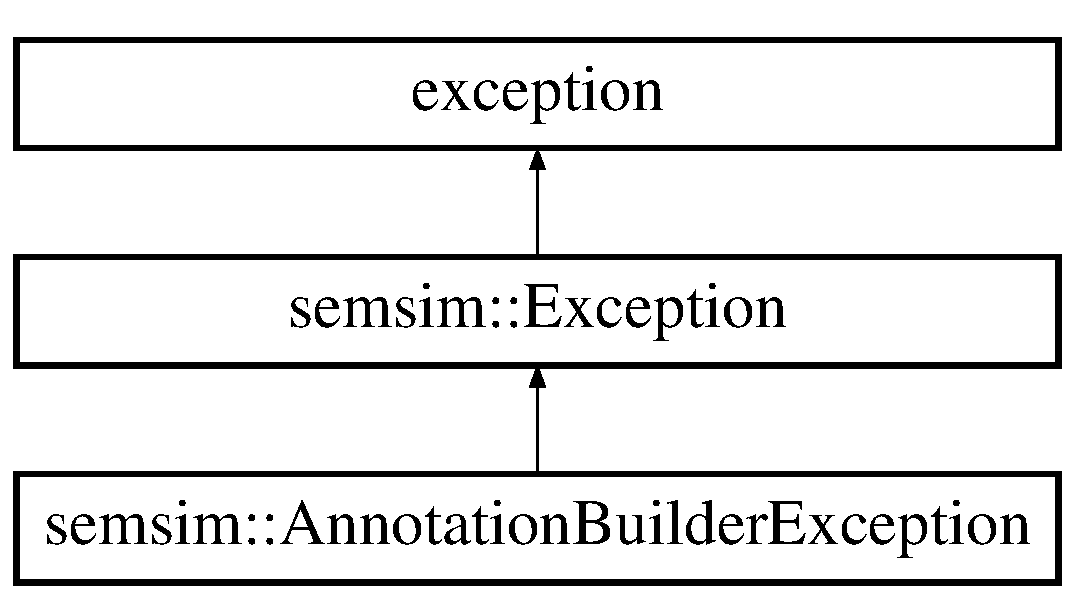
\includegraphics[height=3.000000cm]{classsemsim_1_1AnnotationBuilderException}
                                                                       \end{center}
\end{figure}
\doxysubsection*{Additional Inherited Members}


The documentation for this class was generated from the following file\+:\begin{DoxyCompactItemize}
                                                                             \item
                                                                             src/semsim/Error.\+h
\end{DoxyCompactItemize}

\hypertarget{classsemsim_1_1BiomodelsBiologyQualifier}{}\section{semsim\+:\+:Biomodels\+Biology\+Qualifier Class Reference}
\label{classsemsim_1_1BiomodelsBiologyQualifier}\index{semsim\+::\+Biomodels\+Biology\+Qualifier@{semsim\+::\+Biomodels\+Biology\+Qualifier}}
Inheritance diagram for semsim\+:\+:Biomodels\+Biology\+Qualifier\+:\begin{figure}[H]
\begin{center}
\leavevmode
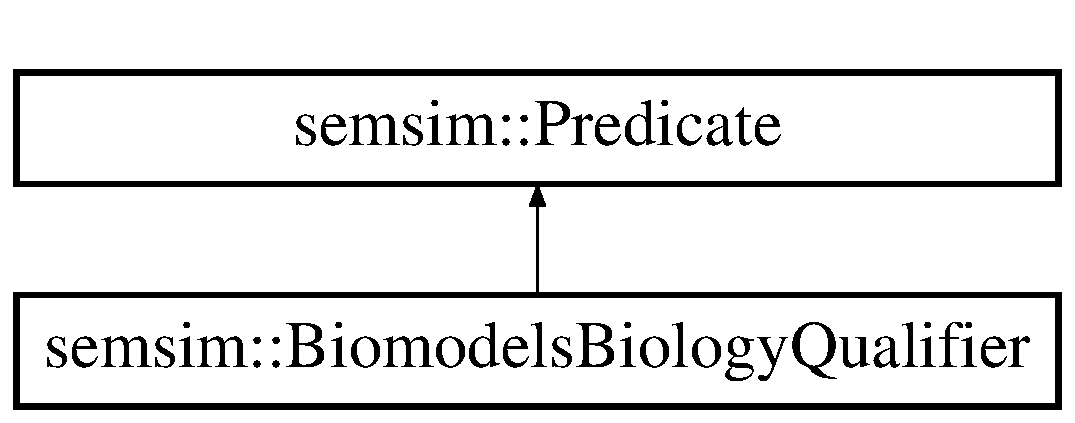
\includegraphics[height=2.000000cm]{classsemsim_1_1BiomodelsBiologyQualifier}
\end{center}
\end{figure}
\subsection*{Public Member Functions}
\begin{DoxyCompactItemize}
\item 
\mbox{\Hypertarget{classsemsim_1_1BiomodelsBiologyQualifier_a0053c8e51b3a7c76ac688e7b2107eef6}\label{classsemsim_1_1BiomodelsBiologyQualifier_a0053c8e51b3a7c76ac688e7b2107eef6}} 
{\bfseries Biomodels\+Biology\+Qualifier} (const std\+::string \&term)
\item 
\mbox{\Hypertarget{classsemsim_1_1BiomodelsBiologyQualifier_a356d84e018e1523321893e71a47b75ef}\label{classsemsim_1_1BiomodelsBiologyQualifier_a356d84e018e1523321893e71a47b75ef}} 
void {\bfseries verify} ()
\end{DoxyCompactItemize}
\subsection*{Public Attributes}
\begin{DoxyCompactItemize}
\item 
std\+::vector$<$ std\+::string $>$ {\bfseries valid\+\_\+terms\+\_\+}
\end{DoxyCompactItemize}
\subsection*{Additional Inherited Members}


\subsection{Member Data Documentation}
\mbox{\Hypertarget{classsemsim_1_1BiomodelsBiologyQualifier_a73a6b7ec962f32c4f03f292f23175440}\label{classsemsim_1_1BiomodelsBiologyQualifier_a73a6b7ec962f32c4f03f292f23175440}} 
\index{semsim\+::\+Biomodels\+Biology\+Qualifier@{semsim\+::\+Biomodels\+Biology\+Qualifier}!valid\+\_\+terms\+\_\+@{valid\+\_\+terms\+\_\+}}
\index{valid\+\_\+terms\+\_\+@{valid\+\_\+terms\+\_\+}!semsim\+::\+Biomodels\+Biology\+Qualifier@{semsim\+::\+Biomodels\+Biology\+Qualifier}}
\subsubsection{\texorpdfstring{valid\+\_\+terms\+\_\+}{valid\_terms\_}}
{\footnotesize\ttfamily std\+::vector$<$std\+::string$>$ semsim\+::\+Biomodels\+Biology\+Qualifier\+::valid\+\_\+terms\+\_\+}

{\bfseries Initial value\+:}
\begin{DoxyCode}
\{
                \textcolor{stringliteral}{"is"},
                \textcolor{stringliteral}{"hasPart"},
                \textcolor{stringliteral}{"isPartOf"},
                \textcolor{stringliteral}{"isVersionOf"},
                \textcolor{stringliteral}{"hasVersion"},
                \textcolor{stringliteral}{"isHomologTo"},
                \textcolor{stringliteral}{"isDescribedBy"},
                \textcolor{stringliteral}{"isEncodedBy"},
                \textcolor{stringliteral}{"encodes"},
                \textcolor{stringliteral}{"occursIn"},
                \textcolor{stringliteral}{"hasProperty"},
                \textcolor{stringliteral}{"isPropertyOf"},
                \textcolor{stringliteral}{"hasTaxon"}
        \}
\end{DoxyCode}


The documentation for this class was generated from the following files\+:\begin{DoxyCompactItemize}
\item 
src/semsim/Predicate.\+h\item 
src/semsim/Predicate.\+cpp\end{DoxyCompactItemize}

\hypertarget{classsemsim_1_1BiomodelsModelQualifier}{}\doxysection{semsim\+::Biomodels\+Model\+Qualifier Class Reference}
\label{classsemsim_1_1BiomodelsModelQualifier}\index{semsim::BiomodelsModelQualifier@{semsim::BiomodelsModelQualifier}}
Inheritance diagram for semsim\+::Biomodels\+Model\+Qualifier\+:\begin{figure}[H]
                                                                    \begin{center}
                                                                        \leavevmode
                                                                        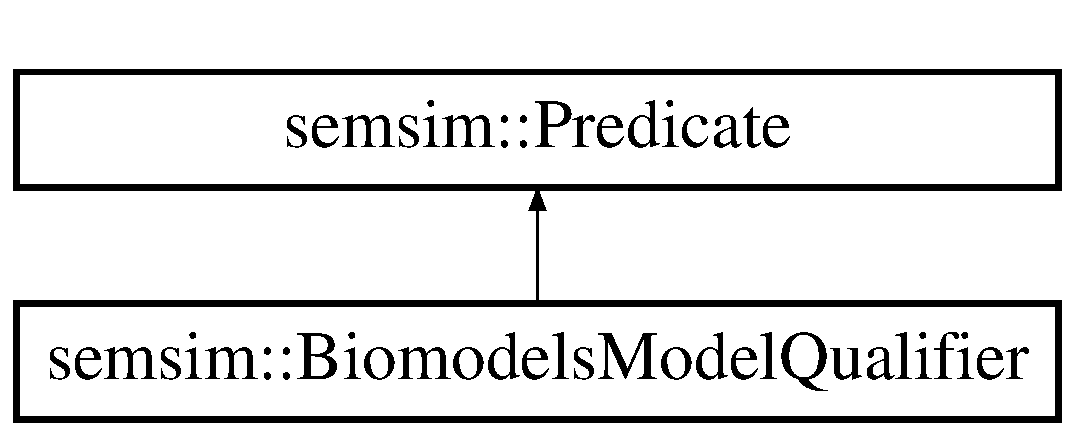
\includegraphics[height=2.000000cm]{classsemsim_1_1BiomodelsModelQualifier}
                                                                    \end{center}
\end{figure}
\doxysubsection*{Public Member Functions}
\begin{DoxyCompactItemize}
    \item
    \mbox{\Hypertarget{classsemsim_1_1BiomodelsModelQualifier_a705462b158ac0ac396bfd6786496d300}\label{classsemsim_1_1BiomodelsModelQualifier_a705462b158ac0ac396bfd6786496d300}}
    {\bfseries Biomodels\+Model\+Qualifier} (Librdf\+World world, const std\+::string \&term)
\end{DoxyCompactItemize}
\doxysubsection*{Public Attributes}
\begin{DoxyCompactItemize}
    \item
    std\+::vector$<$ std\+::string $>$ {\bfseries valid\+\_\+terms\+\_\+}
\end{DoxyCompactItemize}
\doxysubsection*{Additional Inherited Members}


\doxysubsection{Member Data Documentation}
\mbox{\Hypertarget{classsemsim_1_1BiomodelsModelQualifier_a6c270c5a9d8592180253a0e3a1e4f9ae}\label{classsemsim_1_1BiomodelsModelQualifier_a6c270c5a9d8592180253a0e3a1e4f9ae}}
\index{semsim::BiomodelsModelQualifier@{semsim::BiomodelsModelQualifier}!valid\_terms\_@{valid\_terms\_}}
\index{valid\_terms\_@{valid\_terms\_}!semsim::BiomodelsModelQualifier@{semsim::BiomodelsModelQualifier}}
\doxysubsubsection{\texorpdfstring{valid\_terms\_}{valid\_terms\_}}
{\footnotesize\ttfamily std\+::vector$<$std\+::string$>$ semsim\+::\+Biomodels\+Model\+Qualifier\+::valid\+\_\+terms\+\_\+}

{\bfseries Initial value\+:}
\begin{DoxyCode}{0}
    \DoxyCodeLine{\{}
    \DoxyCodeLine{                \textcolor{stringliteral}{"is"},}
    \DoxyCodeLine{                \textcolor{stringliteral}{"isDerivedFrom"},}
    \DoxyCodeLine{                \textcolor{stringliteral}{"isDescribedBy"},}
    \DoxyCodeLine{                \textcolor{stringliteral}{"isInstanceOf"},}
    \DoxyCodeLine{                \textcolor{stringliteral}{"hasInstance"},}
    \DoxyCodeLine{        \}}

\end{DoxyCode}


The documentation for this class was generated from the following files\+:\begin{DoxyCompactItemize}
                                                                              \item
                                                                              src/semsim/Predicate.\+h\item
                                                                              src/semsim/Predicate.\+cpp
\end{DoxyCompactItemize}

\hypertarget{classsemsim_1_1CellMLAssistant}{}\doxysection{semsim\+::Cell\+M\+L\+Assistant Class Reference}
\label{classsemsim_1_1CellMLAssistant}\index{semsim::CellMLAssistant@{semsim::CellMLAssistant}}
Inheritance diagram for semsim\+::Cell\+M\+L\+Assistant\+:\begin{figure}[H]
                                                              \begin{center}
                                                                  \leavevmode
                                                                  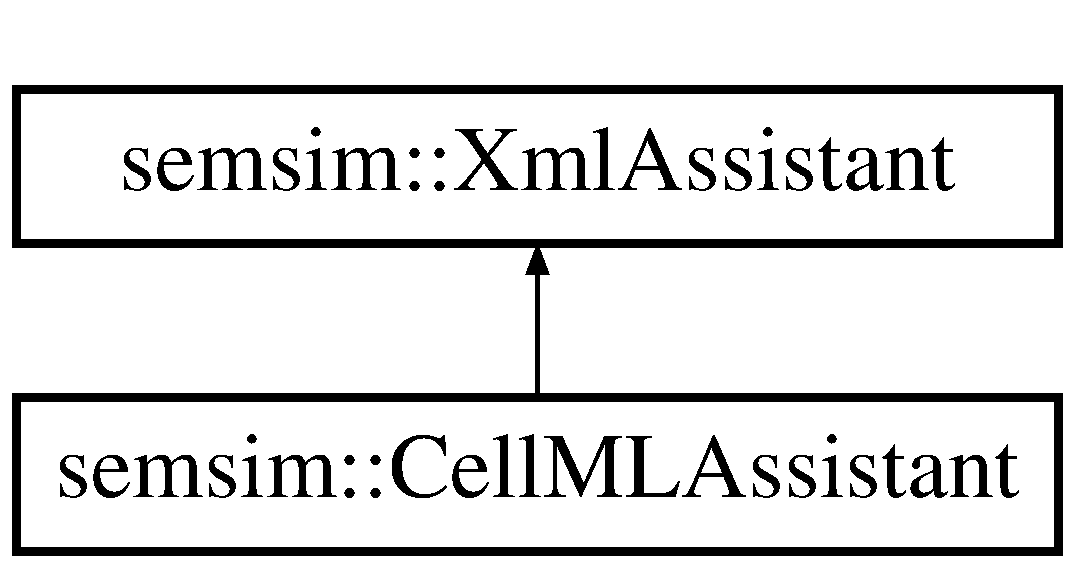
\includegraphics[height=2.000000cm]{classsemsim_1_1CellMLAssistant}
                                                              \end{center}
\end{figure}
\doxysubsection*{Public Member Functions}
\begin{DoxyCompactItemize}
    \item
    \mbox{\Hypertarget{classsemsim_1_1CellMLAssistant_a7c4eb903cc0143fa1d06b7fed802d054}\label{classsemsim_1_1CellMLAssistant_a7c4eb903cc0143fa1d06b7fed802d054}}
    const std\+::vector$<$ std\+::string $>$ \& {\bfseries get\+Valid\+Elements} () const override
    \item
    \mbox{\Hypertarget{classsemsim_1_1CellMLAssistant_a9616a091738c75e94e2ceb9f948f6b51}\label{classsemsim_1_1CellMLAssistant_a9616a091738c75e94e2ceb9f948f6b51}}
    {\bfseries Xml\+Assistant} (std\+::string xml, std\+::string base=\char`\"{}Meta\+ID\char`\"{}, int metaid\+\_\+num\+\_\+digits=4)
\end{DoxyCompactItemize}


The documentation for this class was generated from the following files\+:\begin{DoxyCompactItemize}
                                                                              \item
                                                                              src/semsim/Xml\+Assistant.\+h\item
                                                                              src/semsim/Xml\+Assistant.\+cpp
\end{DoxyCompactItemize}

\hypertarget{classsemsim_1_1CurlGet}{}\doxysection{semsim\+::Curl\+Get Class Reference}
\label{classsemsim_1_1CurlGet}\index{semsim::CurlGet@{semsim::CurlGet}}
\doxysubsection*{Static Public Member Functions}
\begin{DoxyCompactItemize}
    \item
    \mbox{\Hypertarget{classsemsim_1_1CurlGet_ab84cbd76261ce3b191a9442a539fd430}\label{classsemsim_1_1CurlGet_ab84cbd76261ce3b191a9442a539fd430}}
    static int {\bfseries download} (const std\+::string \&url, const std\+::string \&output\+\_\+filename)
\end{DoxyCompactItemize}


The documentation for this class was generated from the following files\+:\begin{DoxyCompactItemize}
                                                                              \item
                                                                              src/semsim/Curl\+Get.\+h\item
                                                                              src/semsim/Curl\+Get.\+cpp
\end{DoxyCompactItemize}

\hypertarget{classsemsim_1_1DCTerm}{}\section{semsim\+:\+:D\+C\+Term Class Reference}
\label{classsemsim_1_1DCTerm}\index{semsim\+::\+D\+C\+Term@{semsim\+::\+D\+C\+Term}}
Inheritance diagram for semsim\+:\+:D\+C\+Term\+:\begin{figure}[H]
\begin{center}
\leavevmode
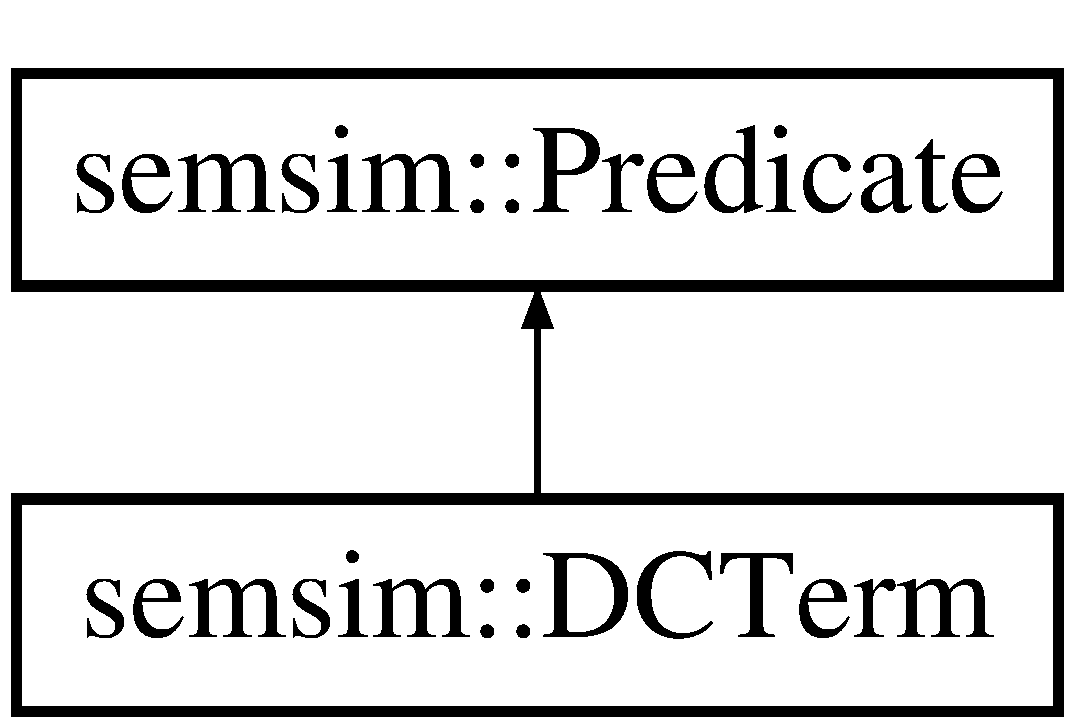
\includegraphics[height=2.000000cm]{classsemsim_1_1DCTerm}
\end{center}
\end{figure}
\subsection*{Public Member Functions}
\begin{DoxyCompactItemize}
\item 
\mbox{\Hypertarget{classsemsim_1_1DCTerm_a7ad576d21a2b4ddca2de1123fc9f5cd1}\label{classsemsim_1_1DCTerm_a7ad576d21a2b4ddca2de1123fc9f5cd1}} 
{\bfseries D\+C\+Term} (const std\+::string \&term)
\item 
\mbox{\Hypertarget{classsemsim_1_1DCTerm_a37a0aeaee6980ec00d51e686f0bd551b}\label{classsemsim_1_1DCTerm_a37a0aeaee6980ec00d51e686f0bd551b}} 
void {\bfseries verify} ()
\end{DoxyCompactItemize}
\subsection*{Public Attributes}
\begin{DoxyCompactItemize}
\item 
std\+::vector$<$ std\+::string $>$ {\bfseries valid\+\_\+terms\+\_\+}
\end{DoxyCompactItemize}
\subsection*{Additional Inherited Members}


\subsection{Member Data Documentation}
\mbox{\Hypertarget{classsemsim_1_1DCTerm_a09e8c38dd1a51c893ed92cca2e675475}\label{classsemsim_1_1DCTerm_a09e8c38dd1a51c893ed92cca2e675475}} 
\index{semsim\+::\+D\+C\+Term@{semsim\+::\+D\+C\+Term}!valid\+\_\+terms\+\_\+@{valid\+\_\+terms\+\_\+}}
\index{valid\+\_\+terms\+\_\+@{valid\+\_\+terms\+\_\+}!semsim\+::\+D\+C\+Term@{semsim\+::\+D\+C\+Term}}
\subsubsection{\texorpdfstring{valid\+\_\+terms\+\_\+}{valid\_terms\_}}
{\footnotesize\ttfamily std\+::vector$<$std\+::string$>$ semsim\+::\+D\+C\+Term\+::valid\+\_\+terms\+\_\+}

{\bfseries Initial value\+:}
\begin{DoxyCode}
\{
                \textcolor{stringliteral}{"Description"}
        \}
\end{DoxyCode}


The documentation for this class was generated from the following files\+:\begin{DoxyCompactItemize}
\item 
src/semsim/Predicate.\+h\item 
src/semsim/Predicate.\+cpp\end{DoxyCompactItemize}

\hypertarget{classsemsim_1_1Editor}{}\doxysection{semsim\+::Editor Class Reference}
\label{classsemsim_1_1Editor}\index{semsim::Editor@{semsim::Editor}}
\doxysubsection*{Public Member Functions}
\begin{DoxyCompactItemize}
    \item
    \mbox{\Hypertarget{classsemsim_1_1Editor_a41935516eed7c1a74d867c7d9001b9d9}\label{classsemsim_1_1Editor_a41935516eed7c1a74d867c7d9001b9d9}}
    const Namespace\+Map \& {\bfseries get\+Namespaces} () const
    \item
    \mbox{\Hypertarget{classsemsim_1_1Editor_a9b264ec07660c5c163a40bedd5ab903e}\label{classsemsim_1_1Editor_a9b264ec07660c5c163a40bedd5ab903e}}
    Librdf\+World {\bfseries get\+World} () const
    \item
    \mbox{\Hypertarget{classsemsim_1_1Editor_a2344dbf9775b1bc5968a7f6816e5e507}\label{classsemsim_1_1Editor_a2344dbf9775b1bc5968a7f6816e5e507}}
    Librdf\+Model {\bfseries get\+Model} () const
    \item
    \mbox{\Hypertarget{classsemsim_1_1Editor_aa67799c71119627bf2eb149777926619}\label{classsemsim_1_1Editor_aa67799c71119627bf2eb149777926619}}
    void {\bfseries set\+Namespaces} (const Namespace\+Map \&namespaces)
    \item
    \mbox{\Hypertarget{classsemsim_1_1Editor_ad807739b96bf8a11cf156cd655640d9e}\label{classsemsim_1_1Editor_ad807739b96bf8a11cf156cd655640d9e}}
    const Nested\+Triples \& {\bfseries get\+Triple\+List} () const
    \item
    \mbox{\Hypertarget{classsemsim_1_1Editor_a9f63d3e365758627b1af3edcd55065ac}\label{classsemsim_1_1Editor_a9f63d3e365758627b1af3edcd55065ac}}
    {\bfseries Editor} (const std\+::string \&xml, Xml\+Assistant\+Type type, Librdf\+World world, Librdf\+Model model, Namespace\+Map \&ns\+\_\+map)
    \item
    \mbox{\Hypertarget{classsemsim_1_1Editor_ac44d2a14cc890ab502897b8147d6a7f0}\label{classsemsim_1_1Editor_ac44d2a14cc890ab502897b8147d6a7f0}}
    const std\+::string \& {\bfseries get\+Xml} () const
    \item
    \mbox{\Hypertarget{classsemsim_1_1Editor_a442a53c7f01042a82307f161a9fb39aa}\label{classsemsim_1_1Editor_a442a53c7f01042a82307f161a9fb39aa}}
    const std\+::vector$<$ std\+::string $>$ \& {\bfseries get\+Metaids} () const
    \item
    \mbox{\Hypertarget{classsemsim_1_1Editor_a52f9cf039194b8aa64a56737398ce158}\label{classsemsim_1_1Editor_a52f9cf039194b8aa64a56737398ce158}}
    void {\bfseries add\+Single\+Annotation} (\mbox{\hyperlink{classsemsim_1_1Subject}{Subject}} subject, Predicate\+Ptr predicate\+\_\+ptr, \mbox{\hyperlink{classsemsim_1_1Resource}{Resource}} resource)
    \item
    \mbox{\Hypertarget{classsemsim_1_1Editor_ac9f7e88c9d94e7f557e0447de9bb80a1}\label{classsemsim_1_1Editor_ac9f7e88c9d94e7f557e0447de9bb80a1}}
    void {\bfseries add\+Namespace} (std\+::string ns, std\+::string prefix)
    \item
    \mbox{\Hypertarget{classsemsim_1_1Editor_ab555e053b2c49e97ab11e873bc38e949}\label{classsemsim_1_1Editor_ab555e053b2c49e97ab11e873bc38e949}}
    void {\bfseries add\+Single\+Annotation} (\mbox{\hyperlink{classsemsim_1_1Triple}{Singular\+Annotation}} singular\+Annotation)
    \item
    \mbox{\Hypertarget{classsemsim_1_1Editor_af4d4f32ca8dd1c7a952ec8887dfaf3d1}\label{classsemsim_1_1Editor_af4d4f32ca8dd1c7a952ec8887dfaf3d1}}
    void {\bfseries add\+Composite\+Annotation} (Physical\+Phenomenon\+Ptr phenomenon\+Ptr)
    \item
    \mbox{\Hypertarget{classsemsim_1_1Editor_abfe645502814173c412af776d3315e33}\label{classsemsim_1_1Editor_abfe645502814173c412af776d3315e33}}
    void {\bfseries add\+Physical\+Entity} (\mbox{\hyperlink{classsemsim_1_1PhysicalEntity}{Physical\+Entity}} physical\+Entity)
    \item
    \mbox{\Hypertarget{classsemsim_1_1Editor_adbe65d49835ddc3034cfb8529b76e50a}\label{classsemsim_1_1Editor_adbe65d49835ddc3034cfb8529b76e50a}}
    void {\bfseries add\+Physical\+Process} (\mbox{\hyperlink{classsemsim_1_1PhysicalProcess}{Physical\+Process}} physical\+Process)
    \item
    \mbox{\Hypertarget{classsemsim_1_1Editor_a7657fbbb87714526dfed15d3ae983350}\label{classsemsim_1_1Editor_a7657fbbb87714526dfed15d3ae983350}}
    void {\bfseries add\+Physical\+Force} (\mbox{\hyperlink{classsemsim_1_1PhysicalForce}{Physical\+Force}} physical\+Force)
    \item
    \mbox{\Hypertarget{classsemsim_1_1Editor_a577a1b6eb322412845f1b6e34b5c9990}\label{classsemsim_1_1Editor_a577a1b6eb322412845f1b6e34b5c9990}}
    void {\bfseries add\+Annotation\+From\+Nested\+Triples} (Nested\+Triples triple\+List)
    \item
    \mbox{\Hypertarget{classsemsim_1_1Editor_ae4d2ddb5f9c637bdaa9b65008bb00dfb}\label{classsemsim_1_1Editor_ae4d2ddb5f9c637bdaa9b65008bb00dfb}}
    void {\bfseries remove\+Annotation} (std\+::string metaid)
    \item
    \mbox{\Hypertarget{classsemsim_1_1Editor_a71f30e2cb766b0ad3ee4ed420cae4109}\label{classsemsim_1_1Editor_a71f30e2cb766b0ad3ee4ed420cae4109}}
    void {\bfseries to\+R\+DF} ()
    \item
    \mbox{\Hypertarget{classsemsim_1_1Editor_a3b02b6bfc728e4c36f74264295fba184}\label{classsemsim_1_1Editor_a3b02b6bfc728e4c36f74264295fba184}}
    void {\bfseries check\+Valid\+Metaid} (const std\+::string \&metaid)
    \item
    \mbox{\Hypertarget{classsemsim_1_1Editor_a05d70846b1d67decebe09a5dddfdf3eb}\label{classsemsim_1_1Editor_a05d70846b1d67decebe09a5dddfdf3eb}}
    void {\bfseries add\+Annotation\+From\+Triples} (\mbox{\hyperlink{classsemsim_1_1Triples}{Triples}} triples)
\end{DoxyCompactItemize}


The documentation for this class was generated from the following files\+:\begin{DoxyCompactItemize}
                                                                              \item
                                                                              src/semsim/Editor.\+h\item
                                                                              src/semsim/Editor.\+cpp
\end{DoxyCompactItemize}

\hypertarget{classException}{}\doxysection{Exception Class Reference}
\label{classException}\index{Exception@{Exception}}
Inheritance diagram for Exception\+:\begin{figure}[H]
\begin{center}
\leavevmode
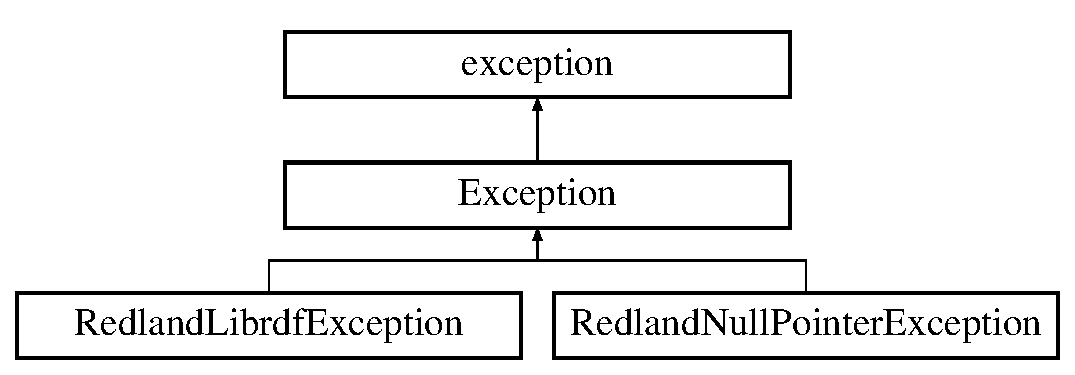
\includegraphics[height=3.000000cm]{classException}
\end{center}
\end{figure}
\doxysubsection*{Public Member Functions}
\begin{DoxyCompactItemize}
\item 
\mbox{\hyperlink{classException_ac541ead5c20548813d7dea73c28c7fab}{Exception}} (const char $\ast$message)
\item 
\mbox{\hyperlink{classException_a0b1693d4d5007815322070c907ee5cc2}{Exception}} (std\+::string message)
\item 
\mbox{\hyperlink{classException_ab834fdbc275748cf287b994503521ada}{$\sim$\+Exception}} () noexcept override=default
\item 
const char $\ast$ \mbox{\hyperlink{classException_ae7ba8334eb35e001b4b0c6df9339c0dc}{what}} () const noexcept override
\end{DoxyCompactItemize}
\doxysubsection*{Protected Attributes}
\begin{DoxyCompactItemize}
\item 
std\+::string \mbox{\hyperlink{classException_a5d59cc46086c61391ed26773ce861780}{msg\+\_\+}}
\end{DoxyCompactItemize}


\doxysubsection{Constructor \& Destructor Documentation}
\mbox{\Hypertarget{classException_ac541ead5c20548813d7dea73c28c7fab}\label{classException_ac541ead5c20548813d7dea73c28c7fab}} 
\index{Exception@{Exception}!Exception@{Exception}}
\index{Exception@{Exception}!Exception@{Exception}}
\doxysubsubsection{\texorpdfstring{Exception()}{Exception()}\hspace{0.1cm}{\footnotesize\ttfamily [1/2]}}
{\footnotesize\ttfamily Exception\+::\+Exception (\begin{DoxyParamCaption}\item[{const char $\ast$}]{message }\end{DoxyParamCaption})\hspace{0.3cm}{\ttfamily [inline]}, {\ttfamily [explicit]}}

Constructor (C strings). 
\begin{DoxyParams}{Parameters}
{\em message} & C-\/style string error message. The string contents are copied upon construction. Hence, responsibility for deleting the char$\ast$ lies with the caller. \\
\hline
\end{DoxyParams}
\mbox{\Hypertarget{classException_a0b1693d4d5007815322070c907ee5cc2}\label{classException_a0b1693d4d5007815322070c907ee5cc2}} 
\index{Exception@{Exception}!Exception@{Exception}}
\index{Exception@{Exception}!Exception@{Exception}}
\doxysubsubsection{\texorpdfstring{Exception()}{Exception()}\hspace{0.1cm}{\footnotesize\ttfamily [2/2]}}
{\footnotesize\ttfamily Exception\+::\+Exception (\begin{DoxyParamCaption}\item[{std\+::string}]{message }\end{DoxyParamCaption})\hspace{0.3cm}{\ttfamily [inline]}, {\ttfamily [explicit]}}

Constructor (C++ STL strings). 
\begin{DoxyParams}{Parameters}
{\em message} & The error message. \\
\hline
\end{DoxyParams}
\mbox{\Hypertarget{classException_ab834fdbc275748cf287b994503521ada}\label{classException_ab834fdbc275748cf287b994503521ada}} 
\index{Exception@{Exception}!````~Exception@{$\sim$Exception}}
\index{````~Exception@{$\sim$Exception}!Exception@{Exception}}
\doxysubsubsection{\texorpdfstring{$\sim$Exception()}{~Exception()}}
{\footnotesize\ttfamily Exception\+::$\sim$\+Exception (\begin{DoxyParamCaption}{ }\end{DoxyParamCaption})\hspace{0.3cm}{\ttfamily [override]}, {\ttfamily [default]}, {\ttfamily [noexcept]}}

Destructor. Virtual to allow for subclassing. 

\doxysubsection{Member Function Documentation}
\mbox{\Hypertarget{classException_ae7ba8334eb35e001b4b0c6df9339c0dc}\label{classException_ae7ba8334eb35e001b4b0c6df9339c0dc}} 
\index{Exception@{Exception}!what@{what}}
\index{what@{what}!Exception@{Exception}}
\doxysubsubsection{\texorpdfstring{what()}{what()}}
{\footnotesize\ttfamily const char$\ast$ Exception\+::what (\begin{DoxyParamCaption}{ }\end{DoxyParamCaption}) const\hspace{0.3cm}{\ttfamily [inline]}, {\ttfamily [override]}, {\ttfamily [noexcept]}}

Returns a pointer to the (constant) error description. \begin{DoxyReturn}{Returns}
A pointer to a const char$\ast$. The underlying memory is in posession of the \mbox{\hyperlink{classException}{Exception}} object. Callers must not attempt to free the memory. 
\end{DoxyReturn}


\doxysubsection{Member Data Documentation}
\mbox{\Hypertarget{classException_a5d59cc46086c61391ed26773ce861780}\label{classException_a5d59cc46086c61391ed26773ce861780}} 
\index{Exception@{Exception}!msg\_@{msg\_}}
\index{msg\_@{msg\_}!Exception@{Exception}}
\doxysubsubsection{\texorpdfstring{msg\_}{msg\_}}
{\footnotesize\ttfamily std\+::string Exception\+::msg\+\_\+\hspace{0.3cm}{\ttfamily [protected]}}

Error message. 

The documentation for this class was generated from the following file\+:\begin{DoxyCompactItemize}
\item 
src/redland/\+Redland\+Wrapper/src/include/redland/Librdf\+Exception.\+h\end{DoxyCompactItemize}

\hypertarget{classsemsim_1_1Exception}{}\section{semsim\+:\+:Exception Class Reference}
\label{classsemsim_1_1Exception}\index{semsim\+::\+Exception@{semsim\+::\+Exception}}


\href{https://stackoverflow.com/questions/8152720/correct-way-to-inherit-from-stdexception}{\tt https\+://stackoverflow.\+com/questions/8152720/correct-\/way-\/to-\/inherit-\/from-\/stdexception}  




{\ttfamily \#include $<$Error.\+h$>$}

Inheritance diagram for semsim\+:\+:Exception\+:\begin{figure}[H]
\begin{center}
\leavevmode
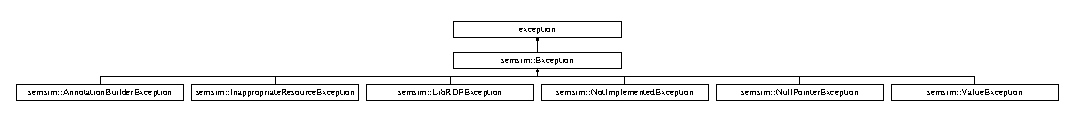
\includegraphics[height=1.120000cm]{classsemsim_1_1Exception}
\end{center}
\end{figure}
\subsection*{Public Member Functions}
\begin{DoxyCompactItemize}
\item 
\hyperlink{classsemsim_1_1Exception_ae32b373f579fc88ca9a9b406327f6549}{Exception} (const char $\ast$message)
\item 
\hyperlink{classsemsim_1_1Exception_acd15baba130b34cb81da8ce237406e99}{Exception} (std\+::string message)
\item 
\hyperlink{classsemsim_1_1Exception_a3f2c9347cddce32086f53f360a7839ae}{$\sim$\+Exception} () noexcept override=default
\item 
const char $\ast$ \hyperlink{classsemsim_1_1Exception_a301e9f6c7020ce7218811f4c0683ee77}{what} () const noexcept override
\end{DoxyCompactItemize}
\subsection*{Protected Attributes}
\begin{DoxyCompactItemize}
\item 
std\+::string \hyperlink{classsemsim_1_1Exception_a536284719db9cd57b8762e6e5a5a8820}{msg\+\_\+}
\end{DoxyCompactItemize}


\subsection{Detailed Description}
\href{https://stackoverflow.com/questions/8152720/correct-way-to-inherit-from-stdexception}{\tt https\+://stackoverflow.\+com/questions/8152720/correct-\/way-\/to-\/inherit-\/from-\/stdexception} 

\subsection{Constructor \& Destructor Documentation}
\mbox{\Hypertarget{classsemsim_1_1Exception_ae32b373f579fc88ca9a9b406327f6549}\label{classsemsim_1_1Exception_ae32b373f579fc88ca9a9b406327f6549}} 
\index{semsim\+::\+Exception@{semsim\+::\+Exception}!Exception@{Exception}}
\index{Exception@{Exception}!semsim\+::\+Exception@{semsim\+::\+Exception}}
\subsubsection{\texorpdfstring{Exception()}{Exception()}\hspace{0.1cm}{\footnotesize\ttfamily [1/2]}}
{\footnotesize\ttfamily semsim\+::\+Exception\+::\+Exception (\begin{DoxyParamCaption}\item[{const char $\ast$}]{message }\end{DoxyParamCaption})\hspace{0.3cm}{\ttfamily [inline]}, {\ttfamily [explicit]}}

Constructor (C strings). 
\begin{DoxyParams}{Parameters}
{\em message} & C-\/style string error message. The string contents are copied upon construction. Hence, responsibility for deleting the char$\ast$ lies with the caller. \\
\hline
\end{DoxyParams}
\mbox{\Hypertarget{classsemsim_1_1Exception_acd15baba130b34cb81da8ce237406e99}\label{classsemsim_1_1Exception_acd15baba130b34cb81da8ce237406e99}} 
\index{semsim\+::\+Exception@{semsim\+::\+Exception}!Exception@{Exception}}
\index{Exception@{Exception}!semsim\+::\+Exception@{semsim\+::\+Exception}}
\subsubsection{\texorpdfstring{Exception()}{Exception()}\hspace{0.1cm}{\footnotesize\ttfamily [2/2]}}
{\footnotesize\ttfamily semsim\+::\+Exception\+::\+Exception (\begin{DoxyParamCaption}\item[{std\+::string}]{message }\end{DoxyParamCaption})\hspace{0.3cm}{\ttfamily [inline]}, {\ttfamily [explicit]}}

Constructor (C++ S\+TL strings). 
\begin{DoxyParams}{Parameters}
{\em message} & The error message. \\
\hline
\end{DoxyParams}
\mbox{\Hypertarget{classsemsim_1_1Exception_a3f2c9347cddce32086f53f360a7839ae}\label{classsemsim_1_1Exception_a3f2c9347cddce32086f53f360a7839ae}} 
\index{semsim\+::\+Exception@{semsim\+::\+Exception}!````~Exception@{$\sim$\+Exception}}
\index{````~Exception@{$\sim$\+Exception}!semsim\+::\+Exception@{semsim\+::\+Exception}}
\subsubsection{\texorpdfstring{$\sim$\+Exception()}{~Exception()}}
{\footnotesize\ttfamily semsim\+::\+Exception\+::$\sim$\+Exception (\begin{DoxyParamCaption}{ }\end{DoxyParamCaption})\hspace{0.3cm}{\ttfamily [override]}, {\ttfamily [default]}, {\ttfamily [noexcept]}}

Destructor. Virtual to allow for subclassing. 

\subsection{Member Function Documentation}
\mbox{\Hypertarget{classsemsim_1_1Exception_a301e9f6c7020ce7218811f4c0683ee77}\label{classsemsim_1_1Exception_a301e9f6c7020ce7218811f4c0683ee77}} 
\index{semsim\+::\+Exception@{semsim\+::\+Exception}!what@{what}}
\index{what@{what}!semsim\+::\+Exception@{semsim\+::\+Exception}}
\subsubsection{\texorpdfstring{what()}{what()}}
{\footnotesize\ttfamily const char$\ast$ semsim\+::\+Exception\+::what (\begin{DoxyParamCaption}{ }\end{DoxyParamCaption}) const\hspace{0.3cm}{\ttfamily [inline]}, {\ttfamily [override]}, {\ttfamily [noexcept]}}

Returns a pointer to the (constant) error description. \begin{DoxyReturn}{Returns}
A pointer to a const char$\ast$. The underlying memory is in posession of the \hyperlink{classsemsim_1_1Exception}{Exception} object. Callers must not attempt to free the memory. 
\end{DoxyReturn}


\subsection{Member Data Documentation}
\mbox{\Hypertarget{classsemsim_1_1Exception_a536284719db9cd57b8762e6e5a5a8820}\label{classsemsim_1_1Exception_a536284719db9cd57b8762e6e5a5a8820}} 
\index{semsim\+::\+Exception@{semsim\+::\+Exception}!msg\+\_\+@{msg\+\_\+}}
\index{msg\+\_\+@{msg\+\_\+}!semsim\+::\+Exception@{semsim\+::\+Exception}}
\subsubsection{\texorpdfstring{msg\+\_\+}{msg\_}}
{\footnotesize\ttfamily std\+::string semsim\+::\+Exception\+::msg\+\_\+\hspace{0.3cm}{\ttfamily [protected]}}

Error message. 

The documentation for this class was generated from the following file\+:\begin{DoxyCompactItemize}
\item 
src/semsim/Error.\+h\end{DoxyCompactItemize}

\hypertarget{classsemsim_1_1InappropriateResourceException}{}\section{semsim\+:\+:Inappropriate\+Resource\+Exception Class Reference}
\label{classsemsim_1_1InappropriateResourceException}\index{semsim\+::\+Inappropriate\+Resource\+Exception@{semsim\+::\+Inappropriate\+Resource\+Exception}}
Inheritance diagram for semsim\+:\+:Inappropriate\+Resource\+Exception\+:\begin{figure}[H]
\begin{center}
\leavevmode
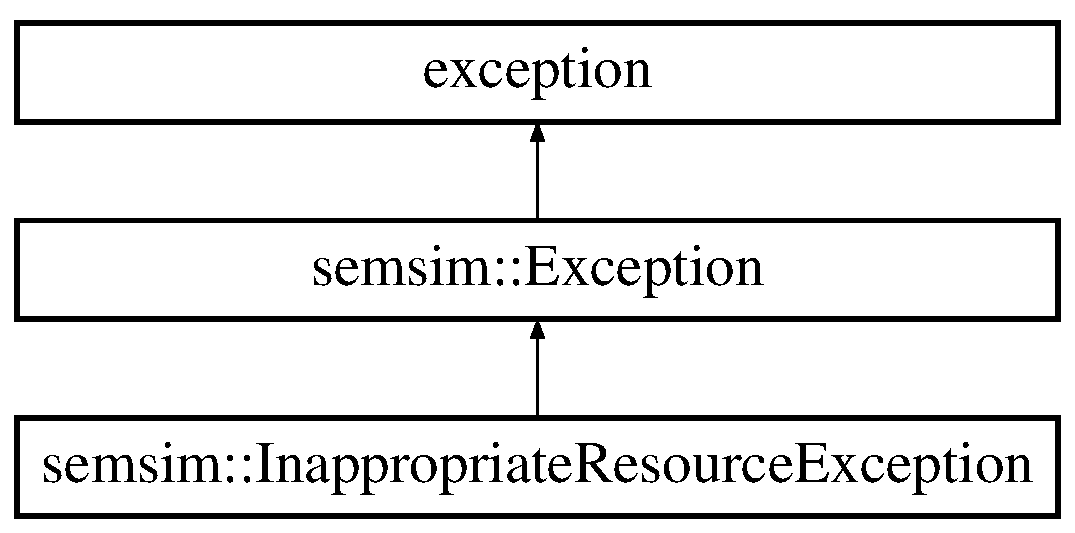
\includegraphics[height=3.000000cm]{classsemsim_1_1InappropriateResourceException}
\end{center}
\end{figure}
\subsection*{Additional Inherited Members}


The documentation for this class was generated from the following file\+:\begin{DoxyCompactItemize}
\item 
src/semsim/Error.\+h\end{DoxyCompactItemize}

\hypertarget{classsemsim_1_1LibRDFException}{}\section{semsim\+:\+:Lib\+R\+D\+F\+Exception Class Reference}
\label{classsemsim_1_1LibRDFException}\index{semsim\+::\+Lib\+R\+D\+F\+Exception@{semsim\+::\+Lib\+R\+D\+F\+Exception}}
Inheritance diagram for semsim\+:\+:Lib\+R\+D\+F\+Exception\+:\begin{figure}[H]
\begin{center}
\leavevmode
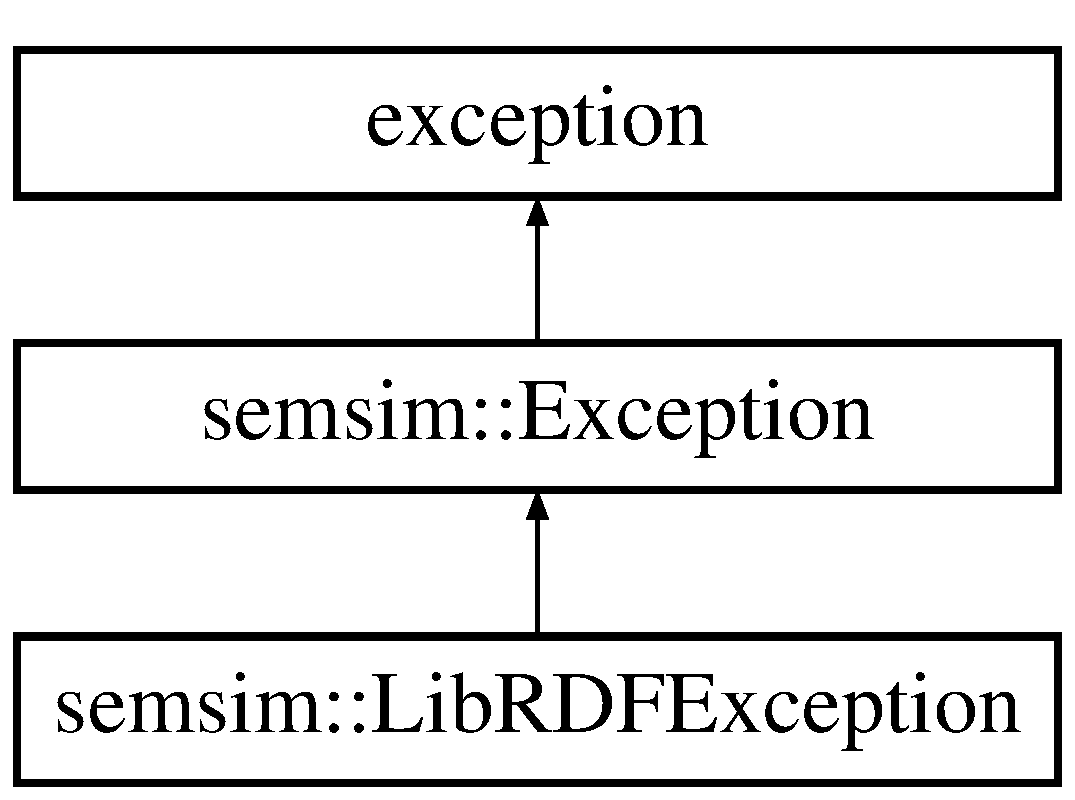
\includegraphics[height=3.000000cm]{classsemsim_1_1LibRDFException}
\end{center}
\end{figure}
\subsection*{Additional Inherited Members}


The documentation for this class was generated from the following file\+:\begin{DoxyCompactItemize}
\item 
src/semsim/Error.\+h\end{DoxyCompactItemize}

\hypertarget{classredland_1_1LibrdfModel}{}\section{redland\+:\+:Librdf\+Model Class Reference}
\label{classredland_1_1LibrdfModel}\index{redland\+::\+Librdf\+Model@{redland\+::\+Librdf\+Model}}
\subsection*{Public Member Functions}
\begin{DoxyCompactItemize}
\item 
\mbox{\Hypertarget{classredland_1_1LibrdfModel_a5a35c032585e38b1d41bc18f057128c1}\label{classredland_1_1LibrdfModel_a5a35c032585e38b1d41bc18f057128c1}} 
{\bfseries Librdf\+Model} (const \hyperlink{classredland_1_1LibrdfModel}{Librdf\+Model} \&model)=delete
\item 
\mbox{\Hypertarget{classredland_1_1LibrdfModel_a583e0eaecfe167ccbbeac5d768bcd644}\label{classredland_1_1LibrdfModel_a583e0eaecfe167ccbbeac5d768bcd644}} 
{\bfseries Librdf\+Model} (\hyperlink{classredland_1_1LibrdfModel}{Librdf\+Model} \&\&model) noexcept
\item 
\mbox{\Hypertarget{classredland_1_1LibrdfModel_a7bd07324b31fa8eb8f5f2e51b15044fc}\label{classredland_1_1LibrdfModel_a7bd07324b31fa8eb8f5f2e51b15044fc}} 
\hyperlink{classredland_1_1LibrdfModel}{Librdf\+Model} \& {\bfseries operator=} (const \hyperlink{classredland_1_1LibrdfModel}{Librdf\+Model} \&model)=delete
\item 
\mbox{\Hypertarget{classredland_1_1LibrdfModel_a9007acfb92943e018d20d6985c811033}\label{classredland_1_1LibrdfModel_a9007acfb92943e018d20d6985c811033}} 
\hyperlink{classredland_1_1LibrdfModel}{Librdf\+Model} \& {\bfseries operator=} (\hyperlink{classredland_1_1LibrdfModel}{Librdf\+Model} \&\&model) noexcept
\item 
\mbox{\Hypertarget{classredland_1_1LibrdfModel_a8b7d3063e030ce8613dcd6def7463a5a}\label{classredland_1_1LibrdfModel_a8b7d3063e030ce8613dcd6def7463a5a}} 
{\bfseries Librdf\+Model} (librdf\+\_\+model $\ast$model)
\item 
\mbox{\Hypertarget{classredland_1_1LibrdfModel_a355e16664fa50a8a3085f4070347106f}\label{classredland_1_1LibrdfModel_a355e16664fa50a8a3085f4070347106f}} 
{\bfseries Librdf\+Model} (librdf\+\_\+storage $\ast$storage, const char $\ast$options=nullptr)
\item 
\mbox{\Hypertarget{classredland_1_1LibrdfModel_ae1b996f1785adfe9b4a1824a73643248}\label{classredland_1_1LibrdfModel_ae1b996f1785adfe9b4a1824a73643248}} 
librdf\+\_\+model $\ast$ {\bfseries get} () const
\item 
\mbox{\Hypertarget{classredland_1_1LibrdfModel_a29e79bafe40a64141ab7edf8ecbbbdd3}\label{classredland_1_1LibrdfModel_a29e79bafe40a64141ab7edf8ecbbbdd3}} 
\hyperlink{classredland_1_1LibrdfQueryResults}{Librdf\+Query\+Results} {\bfseries query} (\hyperlink{classredland_1_1LibrdfQuery}{Librdf\+Query} query)
\item 
\mbox{\Hypertarget{classredland_1_1LibrdfModel_a646ed92896c4030de31c9e17b881bd2a}\label{classredland_1_1LibrdfModel_a646ed92896c4030de31c9e17b881bd2a}} 
\hyperlink{classredland_1_1LibrdfStream}{Librdf\+Stream} {\bfseries to\+Stream} ()
\item 
\mbox{\Hypertarget{classredland_1_1LibrdfModel_a3067eb5bae1353ab5c86f135c4b401ad}\label{classredland_1_1LibrdfModel_a3067eb5bae1353ab5c86f135c4b401ad}} 
int {\bfseries size} () const
\item 
\mbox{\Hypertarget{classredland_1_1LibrdfModel_a2b565a7d705e24d6163c068a40040087}\label{classredland_1_1LibrdfModel_a2b565a7d705e24d6163c068a40040087}} 
void {\bfseries add\+Statement} (const \hyperlink{classredland_1_1LibrdfStatement}{Librdf\+Statement} \&statement) const
\item 
\mbox{\Hypertarget{classredland_1_1LibrdfModel_a643c3e3d3363f4f06330ede73dc19514}\label{classredland_1_1LibrdfModel_a643c3e3d3363f4f06330ede73dc19514}} 
void {\bfseries add\+Statement} (librdf\+\_\+statement $\ast$statement) const
\item 
\mbox{\Hypertarget{classredland_1_1LibrdfModel_ad145b8f46be49434bb8bd0b90a904770}\label{classredland_1_1LibrdfModel_ad145b8f46be49434bb8bd0b90a904770}} 
void {\bfseries free\+Model} ()
\end{DoxyCompactItemize}


The documentation for this class was generated from the following files\+:\begin{DoxyCompactItemize}
\item 
src/redland/\+Redland\+A\+P\+I\+Wrapper/src/Librdf\+Model.\+h\item 
src/redland/\+Redland\+A\+P\+I\+Wrapper/src/Librdf\+Model.\+cpp\end{DoxyCompactItemize}

\hypertarget{classredland_1_1LibrdfNode}{}\doxysection{redland\+::Librdf\+Node Class Reference}
\label{classredland_1_1LibrdfNode}\index{redland::LibrdfNode@{redland::LibrdfNode}}
\doxysubsection*{Public Member Functions}
\begin{DoxyCompactItemize}
\item 
\mbox{\Hypertarget{classredland_1_1LibrdfNode_afc1bdf57705253e8204a394541b96ca7}\label{classredland_1_1LibrdfNode_afc1bdf57705253e8204a394541b96ca7}} 
bool {\bfseries operator==} (const \mbox{\hyperlink{classredland_1_1LibrdfNode}{Librdf\+Node}} \&rhs) const
\item 
\mbox{\Hypertarget{classredland_1_1LibrdfNode_aefbf9e2bf34eb0171932e39323eadfd8}\label{classredland_1_1LibrdfNode_aefbf9e2bf34eb0171932e39323eadfd8}} 
bool {\bfseries operator!=} (const \mbox{\hyperlink{classredland_1_1LibrdfNode}{Librdf\+Node}} \&rhs) const
\item 
\mbox{\Hypertarget{classredland_1_1LibrdfNode_a28f6ce060bddf7e1cb88d17d4d4ea81a}\label{classredland_1_1LibrdfNode_a28f6ce060bddf7e1cb88d17d4d4ea81a}} 
void {\bfseries free\+Node} ()
\item 
\mbox{\Hypertarget{classredland_1_1LibrdfNode_a669557dc1240dc17c3a7a3a61d2400d9}\label{classredland_1_1LibrdfNode_a669557dc1240dc17c3a7a3a61d2400d9}} 
{\bfseries Librdf\+Node} (const \mbox{\hyperlink{classredland_1_1LibrdfNode}{Librdf\+Node}} \&node)=delete
\item 
\mbox{\Hypertarget{classredland_1_1LibrdfNode_a822ce6a4221315abe5768b278b83d0e5}\label{classredland_1_1LibrdfNode_a822ce6a4221315abe5768b278b83d0e5}} 
{\bfseries Librdf\+Node} (\mbox{\hyperlink{classredland_1_1LibrdfNode}{Librdf\+Node}} \&\&node) noexcept
\item 
\mbox{\Hypertarget{classredland_1_1LibrdfNode_abce52c34cc89e48886cde07aa5e113c9}\label{classredland_1_1LibrdfNode_abce52c34cc89e48886cde07aa5e113c9}} 
\mbox{\hyperlink{classredland_1_1LibrdfNode}{Librdf\+Node}} \& {\bfseries operator=} (const \mbox{\hyperlink{classredland_1_1LibrdfNode}{Librdf\+Node}} \&node)=delete
\item 
\mbox{\Hypertarget{classredland_1_1LibrdfNode_a9de3a69b00958b2bb50646dbf0aa8d7e}\label{classredland_1_1LibrdfNode_a9de3a69b00958b2bb50646dbf0aa8d7e}} 
\mbox{\hyperlink{classredland_1_1LibrdfNode}{Librdf\+Node}} \& {\bfseries operator=} (\mbox{\hyperlink{classredland_1_1LibrdfNode}{Librdf\+Node}} \&\&node) noexcept
\item 
\mbox{\Hypertarget{classredland_1_1LibrdfNode_a200c7a67088e66d6fc73f52bdb51d2e9}\label{classredland_1_1LibrdfNode_a200c7a67088e66d6fc73f52bdb51d2e9}} 
{\bfseries Librdf\+Node} (librdf\+\_\+node $\ast$node)
\item 
\mbox{\Hypertarget{classredland_1_1LibrdfNode_a33162ea36efe451c100325816cf8613f}\label{classredland_1_1LibrdfNode_a33162ea36efe451c100325816cf8613f}} 
librdf\+\_\+node $\ast$ {\bfseries get} () const
\item 
\mbox{\Hypertarget{classredland_1_1LibrdfNode_a83ec604f27e71cea80ac49569a06ddfe}\label{classredland_1_1LibrdfNode_a83ec604f27e71cea80ac49569a06ddfe}} 
raptor\+\_\+term\+\_\+type {\bfseries get\+Raptor\+Term\+Type} ()
\item 
\mbox{\Hypertarget{classredland_1_1LibrdfNode_a535fbe1bc21ca9cd9b39b969bfd2e500}\label{classredland_1_1LibrdfNode_a535fbe1bc21ca9cd9b39b969bfd2e500}} 
std\+::string {\bfseries str} () const
\item 
\mbox{\Hypertarget{classredland_1_1LibrdfNode_a98487d5af58971d820fcb99c88d8712d}\label{classredland_1_1LibrdfNode_a98487d5af58971d820fcb99c88d8712d}} 
\mbox{\hyperlink{classredland_1_1LibrdfUri}{Librdf\+Uri}} {\bfseries get\+Literal\+Datatype} ()
\item 
\mbox{\Hypertarget{classredland_1_1LibrdfNode_a58b9962c783be77fd0d2cb7036bfdc6a}\label{classredland_1_1LibrdfNode_a58b9962c783be77fd0d2cb7036bfdc6a}} 
std\+::string {\bfseries get\+Literal\+Language} ()
\item 
\mbox{\Hypertarget{classredland_1_1LibrdfNode_a49431de8c3262ee56d533a5fe047ee00}\label{classredland_1_1LibrdfNode_a49431de8c3262ee56d533a5fe047ee00}} 
std\+::string {\bfseries get\+Blank\+Identifier} ()
\item 
\mbox{\Hypertarget{classredland_1_1LibrdfNode_a0dd2ff697c0753eddf7327f64390ed77}\label{classredland_1_1LibrdfNode_a0dd2ff697c0753eddf7327f64390ed77}} 
\mbox{\hyperlink{classredland_1_1LibrdfUri}{Librdf\+Uri}} {\bfseries get\+Uri} ()
\item 
\mbox{\Hypertarget{classredland_1_1LibrdfNode_a01aeb7675187379674746f803a1fbdc9}\label{classredland_1_1LibrdfNode_a01aeb7675187379674746f803a1fbdc9}} 
void {\bfseries set\+Uri} (const std\+::string \&uri)
\item 
\mbox{\Hypertarget{classredland_1_1LibrdfNode_a160db9f7c7636c339e12c26f519b8fff}\label{classredland_1_1LibrdfNode_a160db9f7c7636c339e12c26f519b8fff}} 
void {\bfseries set\+Literal\+Datatype} (const std\+::string \&datatype)
\item 
\mbox{\Hypertarget{classredland_1_1LibrdfNode_afd81499fe4125cc2f4c472d33fb6c8c0}\label{classredland_1_1LibrdfNode_afd81499fe4125cc2f4c472d33fb6c8c0}} 
void {\bfseries set\+Blank\+Identifier} (const std\+::string \&identifier)
\item 
\mbox{\Hypertarget{classredland_1_1LibrdfNode_a8ac1d280707f4405dc8865465028ae33}\label{classredland_1_1LibrdfNode_a8ac1d280707f4405dc8865465028ae33}} 
\mbox{\hyperlink{classredland_1_1LibrdfNode}{Librdf\+Node}} {\bfseries from\+Uri\+String} (const std\+::string \&uri\+\_\+string, const std\+::string \&local\+\_\+prefix)
\end{DoxyCompactItemize}
\doxysubsection*{Static Public Member Functions}
\begin{DoxyCompactItemize}
\item 
\mbox{\Hypertarget{classredland_1_1LibrdfNode_a5c971e6daeca94c4eabddfa5f6e4c456}\label{classredland_1_1LibrdfNode_a5c971e6daeca94c4eabddfa5f6e4c456}} 
static void {\bfseries free\+Node} (librdf\+\_\+node $\ast$node)
\item 
\mbox{\Hypertarget{classredland_1_1LibrdfNode_aacf853ee60f9d706bc7e95fb426166bd}\label{classredland_1_1LibrdfNode_aacf853ee60f9d706bc7e95fb426166bd}} 
static \mbox{\hyperlink{classredland_1_1LibrdfNode}{Librdf\+Node}} {\bfseries from\+Uri\+String} (const std\+::string \&uri\+\_\+string)
\item 
\mbox{\Hypertarget{classredland_1_1LibrdfNode_a22ea96262be432e6abb5c1e28ede3071}\label{classredland_1_1LibrdfNode_a22ea96262be432e6abb5c1e28ede3071}} 
static \mbox{\hyperlink{classredland_1_1LibrdfNode}{Librdf\+Node}} {\bfseries from\+Blank} (const std\+::string \&blank)
\item 
\mbox{\Hypertarget{classredland_1_1LibrdfNode_a346fad618a010ef983ce24d62891de0e}\label{classredland_1_1LibrdfNode_a346fad618a010ef983ce24d62891de0e}} 
static \mbox{\hyperlink{classredland_1_1LibrdfNode}{Librdf\+Node}} {\bfseries from\+Literal} (const std\+::string \&literal, const std\+::string \&literal\+\_\+datatype\+\_\+uri=\char`\"{}string\char`\"{}, const std\+::string \&xml\+\_\+language=std\+::string())
\item 
\mbox{\Hypertarget{classredland_1_1LibrdfNode_aaeeeca26bafdaf7f118af3307a4768be}\label{classredland_1_1LibrdfNode_aaeeeca26bafdaf7f118af3307a4768be}} 
static \mbox{\hyperlink{classredland_1_1LibrdfNode}{Librdf\+Node}} {\bfseries new\+Empty\+Node} ()
\item 
\mbox{\Hypertarget{classredland_1_1LibrdfNode_aa6bf7e25e68e473f2f39cb7b4cb5f39b}\label{classredland_1_1LibrdfNode_aa6bf7e25e68e473f2f39cb7b4cb5f39b}} 
static std\+::string {\bfseries str} (librdf\+\_\+node $\ast$node)
\item 
\mbox{\Hypertarget{classredland_1_1LibrdfNode_a3242e29edb736ba0aa8ac42fd6b3ae58}\label{classredland_1_1LibrdfNode_a3242e29edb736ba0aa8ac42fd6b3ae58}} 
static std\+::string {\bfseries validate\+Literal\+Datatype} (const std\+::string \&literal\+\_\+datatype\+\_\+uri)
\item 
\mbox{\Hypertarget{classredland_1_1LibrdfNode_a46208d163a49bc7640a8b4c847e2a28b}\label{classredland_1_1LibrdfNode_a46208d163a49bc7640a8b4c847e2a28b}} 
static \mbox{\hyperlink{classredland_1_1LibrdfNode}{Librdf\+Node}} {\bfseries copy\+Node} (const \mbox{\hyperlink{classredland_1_1LibrdfNode}{Librdf\+Node}} \&node)
\item 
\mbox{\Hypertarget{classredland_1_1LibrdfNode_a872032a7516dd140f93a9f4af3e0abd9}\label{classredland_1_1LibrdfNode_a872032a7516dd140f93a9f4af3e0abd9}} 
static \mbox{\hyperlink{classredland_1_1LibrdfNode}{Librdf\+Node}} {\bfseries from\+Relative\+Uri} (const std\+::string \&uri\+\_\+string, const std\+::string \&base\+\_\+uri)
\end{DoxyCompactItemize}


The documentation for this class was generated from the following files\+:\begin{DoxyCompactItemize}
\item 
src/redland/\+Redland\+Wrapper/src/Librdf\+Node.\+h\item 
src/redland/\+Redland\+Wrapper/src/Librdf\+Node.\+cpp\end{DoxyCompactItemize}

\hypertarget{classredland_1_1LibrdfParser}{}\doxysection{redland\+::Librdf\+Parser Class Reference}
\label{classredland_1_1LibrdfParser}\index{redland::LibrdfParser@{redland::LibrdfParser}}
\doxysubsection*{Public Member Functions}
\begin{DoxyCompactItemize}
\item 
\mbox{\Hypertarget{classredland_1_1LibrdfParser_a884b4e7cb05942390fba7765cfb3aec8}\label{classredland_1_1LibrdfParser_a884b4e7cb05942390fba7765cfb3aec8}} 
{\bfseries Librdf\+Parser} (const \mbox{\hyperlink{classredland_1_1LibrdfParser}{Librdf\+Parser}} \&parser)=delete
\item 
\mbox{\Hypertarget{classredland_1_1LibrdfParser_a8c75ee321bd82076491aa0d63d0664c8}\label{classredland_1_1LibrdfParser_a8c75ee321bd82076491aa0d63d0664c8}} 
{\bfseries Librdf\+Parser} (\mbox{\hyperlink{classredland_1_1LibrdfParser}{Librdf\+Parser}} \&\&parser) noexcept
\item 
\mbox{\Hypertarget{classredland_1_1LibrdfParser_aeee1312383f2e3f72e49076390a2a27b}\label{classredland_1_1LibrdfParser_aeee1312383f2e3f72e49076390a2a27b}} 
\mbox{\hyperlink{classredland_1_1LibrdfParser}{Librdf\+Parser}} \& {\bfseries operator=} (const \mbox{\hyperlink{classredland_1_1LibrdfParser}{Librdf\+Parser}} \&parser)=delete
\item 
\mbox{\Hypertarget{classredland_1_1LibrdfParser_a5a5e09075b43906c9161d453ac63ab8a}\label{classredland_1_1LibrdfParser_a5a5e09075b43906c9161d453ac63ab8a}} 
\mbox{\hyperlink{classredland_1_1LibrdfParser}{Librdf\+Parser}} \& {\bfseries operator=} (\mbox{\hyperlink{classredland_1_1LibrdfParser}{Librdf\+Parser}} \&\&parser) noexcept
\item 
\mbox{\Hypertarget{classredland_1_1LibrdfParser_ac1373b22444c108a2a67dbf24fa4ca92}\label{classredland_1_1LibrdfParser_ac1373b22444c108a2a67dbf24fa4ca92}} 
{\bfseries Librdf\+Parser} (librdf\+\_\+parser $\ast$parser)
\item 
\mbox{\Hypertarget{classredland_1_1LibrdfParser_ac594c85ec97a39cad1aa557c98c39eb1}\label{classredland_1_1LibrdfParser_ac594c85ec97a39cad1aa557c98c39eb1}} 
{\bfseries Librdf\+Parser} (std\+::string format, std\+::string mime\+\_\+type=std\+::string(), const std\+::string \&type\+\_\+uri=std\+::string())
\item 
\mbox{\Hypertarget{classredland_1_1LibrdfParser_aadb297b986879ca618d3092fe737d41c}\label{classredland_1_1LibrdfParser_aadb297b986879ca618d3092fe737d41c}} 
librdf\+\_\+parser $\ast$ {\bfseries get} () const
\item 
\mbox{\Hypertarget{classredland_1_1LibrdfParser_a1e2098e2c99ba886ab1521048258600c}\label{classredland_1_1LibrdfParser_a1e2098e2c99ba886ab1521048258600c}} 
int {\bfseries num\+Namespaces\+Seen} () const
\item 
\mbox{\Hypertarget{classredland_1_1LibrdfParser_aed92021f88bccfa26bf78c29797b4208}\label{classredland_1_1LibrdfParser_aed92021f88bccfa26bf78c29797b4208}} 
std\+::string {\bfseries get\+Namespaces\+Seen\+Uri} (int index) const
\item 
\mbox{\Hypertarget{classredland_1_1LibrdfParser_a86739506ba32a9a6da8b69711f1026db}\label{classredland_1_1LibrdfParser_a86739506ba32a9a6da8b69711f1026db}} 
void {\bfseries parse\+String} (const std\+::string \&rdf\+\_\+string, const \mbox{\hyperlink{classredland_1_1LibrdfModel}{Librdf\+Model}} \&model, const \mbox{\hyperlink{classredland_1_1LibrdfUri}{Librdf\+Uri}} \&base\+\_\+uri) const
\item 
\mbox{\Hypertarget{classredland_1_1LibrdfParser_a2a7ac5ac97b4bc5876db02f0b9c7b987}\label{classredland_1_1LibrdfParser_a2a7ac5ac97b4bc5876db02f0b9c7b987}} 
void {\bfseries parse\+String} (const std\+::string \&rdf\+\_\+string, const \mbox{\hyperlink{classredland_1_1LibrdfModel}{Librdf\+Model}} \&model, const std\+::string \&base\+\_\+uri) const
\item 
\mbox{\Hypertarget{classredland_1_1LibrdfParser_a14c24e47699166e3b5bd4141ebd946ff}\label{classredland_1_1LibrdfParser_a14c24e47699166e3b5bd4141ebd946ff}} 
void {\bfseries parse\+File} (const std\+::string \&filename\+\_\+uri, const \mbox{\hyperlink{classredland_1_1LibrdfModel}{Librdf\+Model}} \&model, const std\+::string \&local\+\_\+uri) const
\item 
\mbox{\Hypertarget{classredland_1_1LibrdfParser_a15ffb21bf48e486708eab820719827a6}\label{classredland_1_1LibrdfParser_a15ffb21bf48e486708eab820719827a6}} 
void {\bfseries parse\+File} (const std\+::string \&filename\+\_\+uri, const \mbox{\hyperlink{classredland_1_1LibrdfModel}{Librdf\+Model}} \&model) const
\item 
\mbox{\Hypertarget{classredland_1_1LibrdfParser_a733bf5d33a2d71bd6d7c201e1c952b04}\label{classredland_1_1LibrdfParser_a733bf5d33a2d71bd6d7c201e1c952b04}} 
void {\bfseries parse\+Uri} (const std\+::string \&uri\+\_\+string, const \mbox{\hyperlink{classredland_1_1LibrdfModel}{Librdf\+Model}} \&model) const
\item 
\mbox{\Hypertarget{classredland_1_1LibrdfParser_a89d1335343c9999db8207866de8202c1}\label{classredland_1_1LibrdfParser_a89d1335343c9999db8207866de8202c1}} 
std\+::string {\bfseries get\+Namespaces\+Seen\+Prefix} (int index) const
\item 
\mbox{\Hypertarget{classredland_1_1LibrdfParser_aaa813cd98f57703e2168e81cf1c8b356}\label{classredland_1_1LibrdfParser_aaa813cd98f57703e2168e81cf1c8b356}} 
std\+::string {\bfseries get\+Name} () const
\item 
\mbox{\Hypertarget{classredland_1_1LibrdfParser_a152feb7bf2aa291fc7ec48fe2769265a}\label{classredland_1_1LibrdfParser_a152feb7bf2aa291fc7ec48fe2769265a}} 
void {\bfseries set\+Name} (const char $\ast$name)
\item 
\mbox{\Hypertarget{classredland_1_1LibrdfParser_aacf1514391f15d3687a35352f1c0da3d}\label{classredland_1_1LibrdfParser_aacf1514391f15d3687a35352f1c0da3d}} 
std\+::string {\bfseries get\+Mime\+Type} () const
\item 
\mbox{\Hypertarget{classredland_1_1LibrdfParser_a8fe0e89950e9b71f86fa58e10eb475d8}\label{classredland_1_1LibrdfParser_a8fe0e89950e9b71f86fa58e10eb475d8}} 
void {\bfseries set\+Mime\+Type} (const char $\ast$mime\+Type)
\item 
\mbox{\Hypertarget{classredland_1_1LibrdfParser_ae6f233d632e3a515afe7afceabf4e5ef}\label{classredland_1_1LibrdfParser_ae6f233d632e3a515afe7afceabf4e5ef}} 
librdf\+\_\+uri $\ast$ {\bfseries get\+Type\+Uri} () const
\item 
\mbox{\Hypertarget{classredland_1_1LibrdfParser_a81d772e0be266b00bf840fd9dbeab8d1}\label{classredland_1_1LibrdfParser_a81d772e0be266b00bf840fd9dbeab8d1}} 
void {\bfseries set\+Type\+Uri} (librdf\+\_\+uri $\ast$type\+Uri)
\item 
\mbox{\Hypertarget{classredland_1_1LibrdfParser_a76ecf31cd9fb96ba4e10a35f383e47fc}\label{classredland_1_1LibrdfParser_a76ecf31cd9fb96ba4e10a35f383e47fc}} 
void {\bfseries set\+Type\+Uri} (const std\+::string \&type\+\_\+uri)
\item 
\mbox{\Hypertarget{classredland_1_1LibrdfParser_a8055c22ada8b852112f4f011d9fa5abe}\label{classredland_1_1LibrdfParser_a8055c22ada8b852112f4f011d9fa5abe}} 
librdf\+\_\+parser $\ast$ {\bfseries make\+Parser} ()
\item 
\mbox{\Hypertarget{classredland_1_1LibrdfParser_abca88f90c6d20573961b10800f9b9047}\label{classredland_1_1LibrdfParser_abca88f90c6d20573961b10800f9b9047}} 
std\+::vector$<$ std\+::string $>$ {\bfseries get\+Seen\+Namespaces} (std\+::vector$<$ std\+::string $>$ namespaces) const
\end{DoxyCompactItemize}
\doxysubsection*{Static Public Member Functions}
\begin{DoxyCompactItemize}
\item 
\mbox{\Hypertarget{classredland_1_1LibrdfParser_a9fa0b6b0d21fbc8c6dd0027b66a26eb5}\label{classredland_1_1LibrdfParser_a9fa0b6b0d21fbc8c6dd0027b66a26eb5}} 
static void {\bfseries set\+Feature} (librdf\+\_\+parser $\ast$parser, const std\+::string \&feature\+\_\+uri, \mbox{\hyperlink{structraptor__term}{librdf\+\_\+node}} $\ast$node)
\item 
\mbox{\Hypertarget{classredland_1_1LibrdfParser_aafc4a6e2748ee1175471ed0815d77eff}\label{classredland_1_1LibrdfParser_aafc4a6e2748ee1175471ed0815d77eff}} 
static void {\bfseries set\+Option} (librdf\+\_\+parser $\ast$parser, const std\+::string \&option, const std\+::string \&value)
\item 
\mbox{\Hypertarget{classredland_1_1LibrdfParser_a79fcda1e0c2cccfa8a070a1aea196ebd}\label{classredland_1_1LibrdfParser_a79fcda1e0c2cccfa8a070a1aea196ebd}} 
static void {\bfseries set\+Options} (librdf\+\_\+parser $\ast$parser)
\end{DoxyCompactItemize}


The documentation for this class was generated from the following files\+:\begin{DoxyCompactItemize}
\item 
src/redland/\+Redland\+Wrapper/src/include/redland/Librdf\+Parser.\+h\item 
src/redland/\+Redland\+Wrapper/src/Librdf\+Parser.\+cpp\end{DoxyCompactItemize}

\hypertarget{classredland_1_1LibrdfQuery}{}\doxysection{redland\+::Librdf\+Query Class Reference}
\label{classredland_1_1LibrdfQuery}\index{redland::LibrdfQuery@{redland::LibrdfQuery}}
\doxysubsection*{Public Member Functions}
\begin{DoxyCompactItemize}
\item 
\mbox{\Hypertarget{classredland_1_1LibrdfQuery_aacca5302206092fbd8908934d2236021}\label{classredland_1_1LibrdfQuery_aacca5302206092fbd8908934d2236021}} 
{\bfseries Librdf\+Query} (librdf\+\_\+query $\ast$query)
\item 
\mbox{\Hypertarget{classredland_1_1LibrdfQuery_a63a49930cc3c54938203683eab2c96fb}\label{classredland_1_1LibrdfQuery_a63a49930cc3c54938203683eab2c96fb}} 
{\bfseries Librdf\+Query} (const std\+::string \&query, const std\+::string \&name=\char`\"{}sparql\char`\"{}, const unsigned char $\ast$uri=nullptr, const char $\ast$base\+\_\+uri=nullptr)
\item 
\mbox{\Hypertarget{classredland_1_1LibrdfQuery_a0302f24051ae2050bc2e802a59364554}\label{classredland_1_1LibrdfQuery_a0302f24051ae2050bc2e802a59364554}} 
librdf\+\_\+query $\ast$ {\bfseries get} () const
\end{DoxyCompactItemize}


The documentation for this class was generated from the following files\+:\begin{DoxyCompactItemize}
\item 
src/redland/\+Redland\+Wrapper/src/include/redland/Librdf\+Query.\+h\item 
src/redland/\+Redland\+Wrapper/src/Librdf\+Query.\+cpp\end{DoxyCompactItemize}

\hypertarget{classredland_1_1LibrdfQueryResults}{}\doxysection{redland\+::Librdf\+Query\+Results Class Reference}
\label{classredland_1_1LibrdfQueryResults}\index{redland::LibrdfQueryResults@{redland::LibrdfQueryResults}}
Inheritance diagram for redland\+::Librdf\+Query\+Results\+:\begin{figure}[H]
\begin{center}
\leavevmode
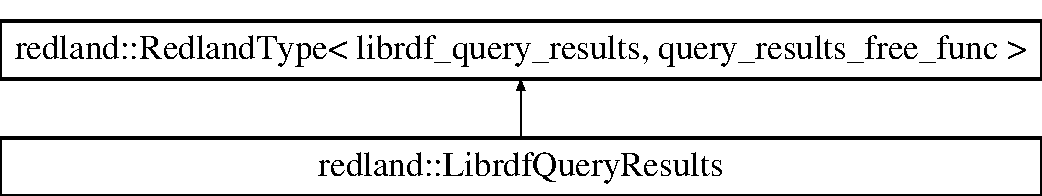
\includegraphics[height=2.000000cm]{classredland_1_1LibrdfQueryResults}
\end{center}
\end{figure}
\doxysubsection*{Public Member Functions}
\begin{DoxyCompactItemize}
\item 
\mbox{\Hypertarget{classredland_1_1LibrdfQueryResults_a8c9e17542c836ff3dd09da68bfc334f1}\label{classredland_1_1LibrdfQueryResults_a8c9e17542c836ff3dd09da68bfc334f1}} 
{\bfseries Librdf\+Query\+Results} (librdf\+\_\+query\+\_\+results $\ast$query\+Results)
\item 
\mbox{\hyperlink{classredland_1_1LibrdfStream}{Librdf\+Stream}} \mbox{\hyperlink{classredland_1_1LibrdfQueryResults_abac7546d8487c786b39046878d27d0b7}{to\+Stream}} ()
\begin{DoxyCompactList}\small\item\em get the query results as a \mbox{\hyperlink{classredland_1_1LibrdfStream}{Librdf\+Stream}} \end{DoxyCompactList}\item 
\mbox{\Hypertarget{classredland_1_1LibrdfQueryResults_a2fc367d8efdeaaa4ebf9e5e710d0440e}\label{classredland_1_1LibrdfQueryResults_a2fc367d8efdeaaa4ebf9e5e710d0440e}} 
int \mbox{\hyperlink{classredland_1_1LibrdfQueryResults_a2fc367d8efdeaaa4ebf9e5e710d0440e}{next}} ()
\begin{DoxyCompactList}\small\item\em Move to the next result. \end{DoxyCompactList}\item 
\mbox{\Hypertarget{classredland_1_1LibrdfQueryResults_ad6ab0b2bd53491ce650f9c740f04c2ec}\label{classredland_1_1LibrdfQueryResults_ad6ab0b2bd53491ce650f9c740f04c2ec}} 
bool \mbox{\hyperlink{classredland_1_1LibrdfQueryResults_ad6ab0b2bd53491ce650f9c740f04c2ec}{is\+Finished}} ()
\begin{DoxyCompactList}\small\item\em true when binding results are exausted \end{DoxyCompactList}\item 
\mbox{\Hypertarget{classredland_1_1LibrdfQueryResults_a1626fe6649dbb8161a05493ac7ec6ee7}\label{classredland_1_1LibrdfQueryResults_a1626fe6649dbb8161a05493ac7ec6ee7}} 
std\+::vector$<$ \mbox{\hyperlink{classredland_1_1LibrdfNode}{Librdf\+Node}} $>$ {\bfseries get\+Bindings} ()
\item 
\mbox{\Hypertarget{classredland_1_1LibrdfQueryResults_a056a92a8cd926072718e4553ed9a39b9}\label{classredland_1_1LibrdfQueryResults_a056a92a8cd926072718e4553ed9a39b9}} 
bool \mbox{\hyperlink{classredland_1_1LibrdfQueryResults_a056a92a8cd926072718e4553ed9a39b9}{is\+Boolean}} ()
\begin{DoxyCompactList}\small\item\em true when this \mbox{\hyperlink{classredland_1_1LibrdfQueryResults}{Librdf\+Query\+Results}} is variable boolean format \end{DoxyCompactList}\item 
\mbox{\Hypertarget{classredland_1_1LibrdfQueryResults_a7a175af6ea28920887c4b2dc4645feb0}\label{classredland_1_1LibrdfQueryResults_a7a175af6ea28920887c4b2dc4645feb0}} 
bool \mbox{\hyperlink{classredland_1_1LibrdfQueryResults_a7a175af6ea28920887c4b2dc4645feb0}{is\+Bindings}} ()
\begin{DoxyCompactList}\small\item\em true when this \mbox{\hyperlink{classredland_1_1LibrdfQueryResults}{Librdf\+Query\+Results}} is variable bindings format \end{DoxyCompactList}\item 
\mbox{\Hypertarget{classredland_1_1LibrdfQueryResults_a52fccc16c398414ddb287fa9bb2a70fd}\label{classredland_1_1LibrdfQueryResults_a52fccc16c398414ddb287fa9bb2a70fd}} 
int {\bfseries get\+Boolean} ()
\item 
\mbox{\Hypertarget{classredland_1_1LibrdfQueryResults_a60e7f4a030655ee3ff0801ce28e3e4e8}\label{classredland_1_1LibrdfQueryResults_a60e7f4a030655ee3ff0801ce28e3e4e8}} 
bool \mbox{\hyperlink{classredland_1_1LibrdfQueryResults_a60e7f4a030655ee3ff0801ce28e3e4e8}{is\+Graph}} ()
\begin{DoxyCompactList}\small\item\em true when this \mbox{\hyperlink{classredland_1_1LibrdfQueryResults}{Librdf\+Query\+Results}} is RDF graph format \end{DoxyCompactList}\item 
\mbox{\Hypertarget{classredland_1_1LibrdfQueryResults_a1a105e783020b8022c5bc8473818be8b}\label{classredland_1_1LibrdfQueryResults_a1a105e783020b8022c5bc8473818be8b}} 
std\+::string {\bfseries get\+Binding\+Value\+By\+Name} (const std\+::string \&name)
\item 
int \mbox{\hyperlink{classredland_1_1LibrdfQueryResults_a1fe7caabdd6e0a2303dd336c9a9b6fb4}{get\+Bindings\+Count}} ()
\begin{DoxyCompactList}\small\item\em returns the number of bindings in the sparql query. \end{DoxyCompactList}\item 
\mbox{\Hypertarget{classredland_1_1LibrdfQueryResults_a6e452fb1c79115834cf97f0898af41f6}\label{classredland_1_1LibrdfQueryResults_a6e452fb1c79115834cf97f0898af41f6}} 
std\+::string {\bfseries to\+String} (const std\+::string \&output\+\_\+format)
\item 
std\+::string \mbox{\hyperlink{classredland_1_1LibrdfQueryResults_ad5f4123f843438e687ef5b8f99816de4}{get\+Bindings\+Name}} (int index)
\begin{DoxyCompactList}\small\item\em get the value of the bindings at \end{DoxyCompactList}\item 
std\+::vector$<$ std\+::string $>$ \mbox{\hyperlink{classredland_1_1LibrdfQueryResults_adf2873cbdc7263b3dd16df61c8ae1c99}{get\+Bindings\+Names}} ()
\begin{DoxyCompactList}\small\item\em get all bindings names as a vector of strings \end{DoxyCompactList}\item 
\mbox{\Hypertarget{classredland_1_1LibrdfQueryResults_a839ea1086c888dbb62c6d5b6d8279add}\label{classredland_1_1LibrdfQueryResults_a839ea1086c888dbb62c6d5b6d8279add}} 
void {\bfseries print\+Query\+Results} ()
\item 
\mbox{\Hypertarget{classredland_1_1LibrdfQueryResults_a856a47ebe225d1d828197f9f2e5c7d9c}\label{classredland_1_1LibrdfQueryResults_a856a47ebe225d1d828197f9f2e5c7d9c}} 
std\+::vector$<$ std\+::string $>$ {\bfseries get\+Valid\+Output\+Formats} () const
\item 
\mbox{\Hypertarget{classredland_1_1LibrdfQueryResults_ac80249e27c57b11309311862c1cee452}\label{classredland_1_1LibrdfQueryResults_ac80249e27c57b11309311862c1cee452}} 
Results\+Map \mbox{\hyperlink{classredland_1_1LibrdfQueryResults_ac80249e27c57b11309311862c1cee452}{map}} ()
\begin{DoxyCompactList}\small\item\em create a map from the query results. \end{DoxyCompactList}\end{DoxyCompactItemize}
\doxysubsection*{Static Public Member Functions}
\begin{DoxyCompactItemize}
\item 
\mbox{\Hypertarget{classredland_1_1LibrdfQueryResults_ad81559675d154f5dd2386ff67d971e46}\label{classredland_1_1LibrdfQueryResults_ad81559675d154f5dd2386ff67d971e46}} 
static std\+::string {\bfseries string\+Replace} (std\+::string str, const std\+::string \&string\+\_\+to\+\_\+replace, const std\+::string \&replacement)
\end{DoxyCompactItemize}
\doxysubsection*{Additional Inherited Members}


\doxysubsection{Member Function Documentation}
\mbox{\Hypertarget{classredland_1_1LibrdfQueryResults_a1fe7caabdd6e0a2303dd336c9a9b6fb4}\label{classredland_1_1LibrdfQueryResults_a1fe7caabdd6e0a2303dd336c9a9b6fb4}} 
\index{redland::LibrdfQueryResults@{redland::LibrdfQueryResults}!getBindingsCount@{getBindingsCount}}
\index{getBindingsCount@{getBindingsCount}!redland::LibrdfQueryResults@{redland::LibrdfQueryResults}}
\doxysubsubsection{\texorpdfstring{getBindingsCount()}{getBindingsCount()}}
{\footnotesize\ttfamily int redland\+::\+Librdf\+Query\+Results\+::get\+Bindings\+Count (\begin{DoxyParamCaption}{ }\end{DoxyParamCaption})}



returns the number of bindings in the sparql query. 

i.\+e. the query SELECT ?x ?y ?z WHERE \{ ?x ?y ?z \} has 3 bindings, x, y and z. \mbox{\Hypertarget{classredland_1_1LibrdfQueryResults_ad5f4123f843438e687ef5b8f99816de4}\label{classredland_1_1LibrdfQueryResults_ad5f4123f843438e687ef5b8f99816de4}} 
\index{redland::LibrdfQueryResults@{redland::LibrdfQueryResults}!getBindingsName@{getBindingsName}}
\index{getBindingsName@{getBindingsName}!redland::LibrdfQueryResults@{redland::LibrdfQueryResults}}
\doxysubsubsection{\texorpdfstring{getBindingsName()}{getBindingsName()}}
{\footnotesize\ttfamily std\+::string redland\+::\+Librdf\+Query\+Results\+::get\+Bindings\+Name (\begin{DoxyParamCaption}\item[{int}]{index }\end{DoxyParamCaption})}



get the value of the bindings at 


\begin{DoxyParams}{Parameters}
{\em index} & as a std\+::string \\
\hline
\end{DoxyParams}
\mbox{\Hypertarget{classredland_1_1LibrdfQueryResults_adf2873cbdc7263b3dd16df61c8ae1c99}\label{classredland_1_1LibrdfQueryResults_adf2873cbdc7263b3dd16df61c8ae1c99}} 
\index{redland::LibrdfQueryResults@{redland::LibrdfQueryResults}!getBindingsNames@{getBindingsNames}}
\index{getBindingsNames@{getBindingsNames}!redland::LibrdfQueryResults@{redland::LibrdfQueryResults}}
\doxysubsubsection{\texorpdfstring{getBindingsNames()}{getBindingsNames()}}
{\footnotesize\ttfamily std\+::vector$<$ std\+::string $>$ redland\+::\+Librdf\+Query\+Results\+::get\+Bindings\+Names (\begin{DoxyParamCaption}{ }\end{DoxyParamCaption})}



get all bindings names as a vector of strings 

the number of bindings is determined by get\+Bindings\+Count \mbox{\Hypertarget{classredland_1_1LibrdfQueryResults_abac7546d8487c786b39046878d27d0b7}\label{classredland_1_1LibrdfQueryResults_abac7546d8487c786b39046878d27d0b7}} 
\index{redland::LibrdfQueryResults@{redland::LibrdfQueryResults}!toStream@{toStream}}
\index{toStream@{toStream}!redland::LibrdfQueryResults@{redland::LibrdfQueryResults}}
\doxysubsubsection{\texorpdfstring{toStream()}{toStream()}}
{\footnotesize\ttfamily \mbox{\hyperlink{classredland_1_1LibrdfStream}{Librdf\+Stream}} redland\+::\+Librdf\+Query\+Results\+::to\+Stream (\begin{DoxyParamCaption}{ }\end{DoxyParamCaption})}



get the query results as a \mbox{\hyperlink{classredland_1_1LibrdfStream}{Librdf\+Stream}} 

only meaningful if this is an RDF graph query result 
\begin{DoxyExceptions}{Exceptions}
{\em invalid\+\_\+argument} & when to\+Stream is called and Librdf\+Query\+Result\+::is\+Graph() evaluates to false. \\
\hline
\end{DoxyExceptions}


The documentation for this class was generated from the following files\+:\begin{DoxyCompactItemize}
\item 
src/redland/\+Redland\+Wrapper/src/include/redland/Librdf\+Query\+Results.\+h\item 
src/redland/\+Redland\+Wrapper/src/Librdf\+Query\+Results.\+cpp\end{DoxyCompactItemize}

\hypertarget{classredland_1_1LibrdfSerializer}{}\doxysection{redland\+::Librdf\+Serializer Class Reference}
\label{classredland_1_1LibrdfSerializer}\index{redland::LibrdfSerializer@{redland::LibrdfSerializer}}
\doxysubsection*{Public Member Functions}
\begin{DoxyCompactItemize}
\item 
\mbox{\Hypertarget{classredland_1_1LibrdfSerializer_a084920f2dadf9aff9abff2fbe4e302e9}\label{classredland_1_1LibrdfSerializer_a084920f2dadf9aff9abff2fbe4e302e9}} 
{\bfseries Librdf\+Serializer} (const \mbox{\hyperlink{classredland_1_1LibrdfSerializer}{Librdf\+Serializer}} \&serializer)=delete
\item 
\mbox{\Hypertarget{classredland_1_1LibrdfSerializer_ac0df7aa8f6a63de75d63f33d9eb3b201}\label{classredland_1_1LibrdfSerializer_ac0df7aa8f6a63de75d63f33d9eb3b201}} 
{\bfseries Librdf\+Serializer} (\mbox{\hyperlink{classredland_1_1LibrdfSerializer}{Librdf\+Serializer}} \&\&serializer) noexcept
\item 
\mbox{\Hypertarget{classredland_1_1LibrdfSerializer_a07c9ec356305e42c4990357dffb6bfd1}\label{classredland_1_1LibrdfSerializer_a07c9ec356305e42c4990357dffb6bfd1}} 
\mbox{\hyperlink{classredland_1_1LibrdfSerializer}{Librdf\+Serializer}} \& {\bfseries operator=} (const \mbox{\hyperlink{classredland_1_1LibrdfSerializer}{Librdf\+Serializer}} \&serializer)=delete
\item 
\mbox{\Hypertarget{classredland_1_1LibrdfSerializer_a3f1049838f6c9b3baee42fd1ab99d9e3}\label{classredland_1_1LibrdfSerializer_a3f1049838f6c9b3baee42fd1ab99d9e3}} 
\mbox{\hyperlink{classredland_1_1LibrdfSerializer}{Librdf\+Serializer}} \& {\bfseries operator=} (\mbox{\hyperlink{classredland_1_1LibrdfSerializer}{Librdf\+Serializer}} \&\&serializer) noexcept
\item 
\mbox{\Hypertarget{classredland_1_1LibrdfSerializer_aadcc241a243f87fce5152dc6420d1625}\label{classredland_1_1LibrdfSerializer_aadcc241a243f87fce5152dc6420d1625}} 
{\bfseries Librdf\+Serializer} (const char $\ast$format, const char $\ast$mime\+\_\+type=nullptr, const char $\ast$type\+\_\+uri=nullptr)
\item 
\mbox{\Hypertarget{classredland_1_1LibrdfSerializer_ab5ef7eaa294357a931b826acc1ab932f}\label{classredland_1_1LibrdfSerializer_ab5ef7eaa294357a931b826acc1ab932f}} 
librdf\+\_\+serializer $\ast$ {\bfseries get} () const
\item 
\mbox{\Hypertarget{classredland_1_1LibrdfSerializer_ab621a575b7244c9d39e756b5e133766b}\label{classredland_1_1LibrdfSerializer_ab621a575b7244c9d39e756b5e133766b}} 
void {\bfseries set\+Namespace} (const std\+::string \&ns, const std\+::string \&prefix) const
\item 
\mbox{\Hypertarget{classredland_1_1LibrdfSerializer_abe500f5c5a1de1bdac86ab196a002b46}\label{classredland_1_1LibrdfSerializer_abe500f5c5a1de1bdac86ab196a002b46}} 
void {\bfseries set\+Feature} (const std\+::string \&ns, const std\+::string \&prefix) const
\item 
\mbox{\Hypertarget{classredland_1_1LibrdfSerializer_ac205990ca1dbf0ff1e56ea45e82ec8d2}\label{classredland_1_1LibrdfSerializer_ac205990ca1dbf0ff1e56ea45e82ec8d2}} 
std\+::string {\bfseries to\+String} (const std\+::string \&uri, const \mbox{\hyperlink{classredland_1_1LibrdfModel}{Librdf\+Model}} \&model)
\item 
\mbox{\Hypertarget{classredland_1_1LibrdfSerializer_aa185a5c5708bf4b08dfa5eb6a8b897b1}\label{classredland_1_1LibrdfSerializer_aa185a5c5708bf4b08dfa5eb6a8b897b1}} 
void {\bfseries free\+Serializer} ()
\item 
\mbox{\Hypertarget{classredland_1_1LibrdfSerializer_a4ea50f1f63c3cb7bb63da3fc55994fee}\label{classredland_1_1LibrdfSerializer_a4ea50f1f63c3cb7bb63da3fc55994fee}} 
void {\bfseries validate\+Serializer\+Name} (std\+::string name)
\item 
\mbox{\Hypertarget{classredland_1_1LibrdfSerializer_a970fa3d23ba08a63533c758417de1808}\label{classredland_1_1LibrdfSerializer_a970fa3d23ba08a63533c758417de1808}} 
void {\bfseries set\+Option} (const std\+::string \&option, const std\+::string \&value) const
\item 
\mbox{\Hypertarget{classredland_1_1LibrdfSerializer_ad2cb2ddcd225119a2a9a33001da22478}\label{classredland_1_1LibrdfSerializer_ad2cb2ddcd225119a2a9a33001da22478}} 
void {\bfseries set\+Options} () const
\end{DoxyCompactItemize}
\doxysubsection*{Static Public Member Functions}
\begin{DoxyCompactItemize}
\item 
\mbox{\Hypertarget{classredland_1_1LibrdfSerializer_a58915bb2aa6b7c0eb438b5cc0148ef45}\label{classredland_1_1LibrdfSerializer_a58915bb2aa6b7c0eb438b5cc0148ef45}} 
static \mbox{\hyperlink{classredland_1_1LibrdfSerializer}{Librdf\+Serializer}} {\bfseries from\+Raw\+Ptr} (librdf\+\_\+serializer $\ast$serializer)
\end{DoxyCompactItemize}


The documentation for this class was generated from the following files\+:\begin{DoxyCompactItemize}
\item 
src/redland/\+Redland\+Wrapper/src/Librdf\+Serializer.\+h\item 
src/redland/\+Redland\+Wrapper/src/Librdf\+Serializer.\+cpp\end{DoxyCompactItemize}

\hypertarget{classredland_1_1LibrdfStatement}{}\doxysection{redland\+::Librdf\+Statement Class Reference}
\label{classredland_1_1LibrdfStatement}\index{redland::LibrdfStatement@{redland::LibrdfStatement}}


C++ wrapper around librdf\+\_\+statement using RAII for memory management.  




{\ttfamily \#include $<$Librdf\+Statement.\+h$>$}

Inheritance diagram for redland\+::Librdf\+Statement\+:\begin{figure}[H]
\begin{center}
\leavevmode
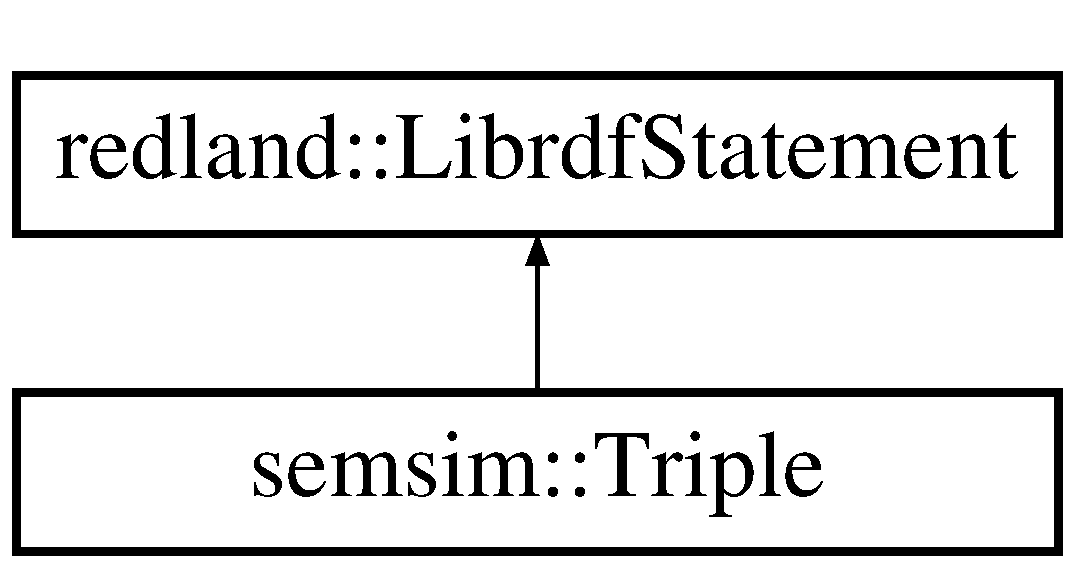
\includegraphics[height=4.000000cm]{classredland_1_1LibrdfStatement}
\end{center}
\end{figure}
\doxysubsection*{Public Member Functions}
\begin{DoxyCompactItemize}
\item 
\mbox{\hyperlink{classredland_1_1LibrdfStatement_a4cbbbf99d094cea4569324a8c67789fb}{Librdf\+Statement}} (\mbox{\hyperlink{structraptor__statement}{librdf\+\_\+statement}} $\ast$statement)
\begin{DoxyCompactList}\small\item\em construct a \mbox{\hyperlink{classredland_1_1LibrdfStatement}{Librdf\+Statement}} from an existing librdf\+\_\+statement$\ast$ pointer. \end{DoxyCompactList}\item 
\mbox{\hyperlink{classredland_1_1LibrdfStatement_a65d896e0bf026ff027ad8488bddf6384}{Librdf\+Statement}} ()
\begin{DoxyCompactList}\small\item\em default construct an instance of librdf\+\_\+statement$\ast$. \end{DoxyCompactList}\item 
\mbox{\Hypertarget{classredland_1_1LibrdfStatement_ada81e9bfb312e25daf20d6dda10eeb2e}\label{classredland_1_1LibrdfStatement_ada81e9bfb312e25daf20d6dda10eeb2e}} 
bool \mbox{\hyperlink{classredland_1_1LibrdfStatement_ada81e9bfb312e25daf20d6dda10eeb2e}{operator==}} (const \mbox{\hyperlink{classredland_1_1LibrdfStatement}{Librdf\+Statement}} \&rhs) const
\begin{DoxyCompactList}\small\item\em equality operator. @detials equal if the three nodes contained by this statement are equal \end{DoxyCompactList}\item 
\mbox{\Hypertarget{classredland_1_1LibrdfStatement_ad3d6c126b90c0d93413a08353c496f8f}\label{classredland_1_1LibrdfStatement_ad3d6c126b90c0d93413a08353c496f8f}} 
bool \mbox{\hyperlink{classredland_1_1LibrdfStatement_ad3d6c126b90c0d93413a08353c496f8f}{operator!=}} (const \mbox{\hyperlink{classredland_1_1LibrdfStatement}{Librdf\+Statement}} \&rhs) const
\begin{DoxyCompactList}\small\item\em inequality operator. Inverse of equality operator \end{DoxyCompactList}\item 
\mbox{\hyperlink{classredland_1_1LibrdfStatement_ae7f7e27b7a502070195103268407243a}{Librdf\+Statement}} (const \mbox{\hyperlink{classredland_1_1LibrdfNode}{Librdf\+Node}} \&subject, const \mbox{\hyperlink{classredland_1_1LibrdfNode}{Librdf\+Node}} \&predicate, const \mbox{\hyperlink{classredland_1_1LibrdfNode}{Librdf\+Node}} \&resource)
\begin{DoxyCompactList}\small\item\em construct a \mbox{\hyperlink{classredland_1_1LibrdfStatement}{Librdf\+Statement}} from \mbox{\hyperlink{classredland_1_1LibrdfNode}{Librdf\+Node}} objects. \end{DoxyCompactList}\item 
\mbox{\hyperlink{classredland_1_1LibrdfNode}{Librdf\+Node}} \mbox{\hyperlink{classredland_1_1LibrdfStatement_a2d7cc313572ac34e9822e97d6b23dd36}{get\+Subject\+Node}} () const
\begin{DoxyCompactList}\small\item\em get the subject of this statement as a \mbox{\hyperlink{classredland_1_1LibrdfNode}{Librdf\+Node}}. \end{DoxyCompactList}\item 
\mbox{\hyperlink{classredland_1_1LibrdfNode}{Librdf\+Node}} \mbox{\hyperlink{classredland_1_1LibrdfStatement_ade668892ca9383eacbf5517df4e8f8d8}{get\+Predicate\+Node}} () const
\begin{DoxyCompactList}\small\item\em get the predicate of this statement as a \mbox{\hyperlink{classredland_1_1LibrdfNode}{Librdf\+Node}}. \end{DoxyCompactList}\item 
\mbox{\hyperlink{classredland_1_1LibrdfNode}{Librdf\+Node}} \mbox{\hyperlink{classredland_1_1LibrdfStatement_a9d4376221d84e22d15eeb6393ea4afe3}{get\+Resource\+Node}} () const
\begin{DoxyCompactList}\small\item\em get the resource of this statement as a \mbox{\hyperlink{classredland_1_1LibrdfNode}{Librdf\+Node}}. \end{DoxyCompactList}\item 
\mbox{\Hypertarget{classredland_1_1LibrdfStatement_a4935cf54fa2f367678319f1f2d837005}\label{classredland_1_1LibrdfStatement_a4935cf54fa2f367678319f1f2d837005}} 
void \mbox{\hyperlink{classredland_1_1LibrdfStatement_a4935cf54fa2f367678319f1f2d837005}{check\+For\+Null}} () override
\begin{DoxyCompactList}\small\item\em throws an error if any of the subject, predicate, resource or librdf\+\_\+statement are nullptr. \end{DoxyCompactList}\item 
void \mbox{\hyperlink{classredland_1_1LibrdfStatement_a9133d53a9b24ac0f0499f23cb6e53d40}{set\+Subject}} (const \mbox{\hyperlink{classredland_1_1LibrdfNode}{Librdf\+Node}} \&node)
\begin{DoxyCompactList}\small\item\em set the subject of this \mbox{\hyperlink{classredland_1_1LibrdfStatement}{Librdf\+Statement}} to node. \end{DoxyCompactList}\item 
void \mbox{\hyperlink{classredland_1_1LibrdfStatement_a74151d5fae756918cfd9b22d51fb8d71}{set\+Resource}} (const \mbox{\hyperlink{classredland_1_1LibrdfNode}{Librdf\+Node}} \&node)
\begin{DoxyCompactList}\small\item\em set the resource of this \mbox{\hyperlink{classredland_1_1LibrdfStatement}{Librdf\+Statement}} to node. \end{DoxyCompactList}\item 
void \mbox{\hyperlink{classredland_1_1LibrdfStatement_a155e25bff7660b03c4253715fe5e8194}{set\+Predicate}} (const \mbox{\hyperlink{classredland_1_1LibrdfNode}{Librdf\+Node}} \&node)
\begin{DoxyCompactList}\small\item\em set the predicate of this \mbox{\hyperlink{classredland_1_1LibrdfStatement}{Librdf\+Statement}} to node. \end{DoxyCompactList}\item 
\mbox{\Hypertarget{classredland_1_1LibrdfStatement_a84a6fae7f1879c2f033001a9927627b0}\label{classredland_1_1LibrdfStatement_a84a6fae7f1879c2f033001a9927627b0}} 
bool \mbox{\hyperlink{classredland_1_1LibrdfStatement_a84a6fae7f1879c2f033001a9927627b0}{is\+Complete}} ()
\begin{DoxyCompactList}\small\item\em returns true when all of subject, predicate and resource nodes are not empty. \end{DoxyCompactList}\end{DoxyCompactItemize}
\doxysubsection*{Static Public Member Functions}
\begin{DoxyCompactItemize}
\item 
static bool \mbox{\hyperlink{classredland_1_1LibrdfStatement_ac5acd1a9c67a8bd6f7b99098a7353424}{equals}} (const \mbox{\hyperlink{classredland_1_1LibrdfStatement}{Librdf\+Statement}} \&first, const \mbox{\hyperlink{classredland_1_1LibrdfStatement}{Librdf\+Statement}} \&second)
\begin{DoxyCompactList}\small\item\em returns true if first equals second. \end{DoxyCompactList}\end{DoxyCompactItemize}
\doxysubsection*{Additional Inherited Members}


\doxysubsection{Detailed Description}
C++ wrapper around librdf\+\_\+statement using RAII for memory management. 

\doxysubsection{Constructor \& Destructor Documentation}
\mbox{\Hypertarget{classredland_1_1LibrdfStatement_a4cbbbf99d094cea4569324a8c67789fb}\label{classredland_1_1LibrdfStatement_a4cbbbf99d094cea4569324a8c67789fb}} 
\index{redland::LibrdfStatement@{redland::LibrdfStatement}!LibrdfStatement@{LibrdfStatement}}
\index{LibrdfStatement@{LibrdfStatement}!redland::LibrdfStatement@{redland::LibrdfStatement}}
\doxysubsubsection{\texorpdfstring{LibrdfStatement()}{LibrdfStatement()}\hspace{0.1cm}{\footnotesize\ttfamily [1/3]}}
{\footnotesize\ttfamily redland\+::\+Librdf\+Statement\+::\+Librdf\+Statement (\begin{DoxyParamCaption}\item[{\mbox{\hyperlink{structraptor__statement}{librdf\+\_\+statement}} $\ast$}]{statement }\end{DoxyParamCaption})\hspace{0.3cm}{\ttfamily [explicit]}}



construct a \mbox{\hyperlink{classredland_1_1LibrdfStatement}{Librdf\+Statement}} from an existing librdf\+\_\+statement$\ast$ pointer. 

The reference is stolen, and subsequently managed by \mbox{\hyperlink{classredland_1_1LibrdfStatement}{Librdf\+Statement}} \mbox{\Hypertarget{classredland_1_1LibrdfStatement_a65d896e0bf026ff027ad8488bddf6384}\label{classredland_1_1LibrdfStatement_a65d896e0bf026ff027ad8488bddf6384}} 
\index{redland::LibrdfStatement@{redland::LibrdfStatement}!LibrdfStatement@{LibrdfStatement}}
\index{LibrdfStatement@{LibrdfStatement}!redland::LibrdfStatement@{redland::LibrdfStatement}}
\doxysubsubsection{\texorpdfstring{LibrdfStatement()}{LibrdfStatement()}\hspace{0.1cm}{\footnotesize\ttfamily [2/3]}}
{\footnotesize\ttfamily redland\+::\+Librdf\+Statement\+::\+Librdf\+Statement (\begin{DoxyParamCaption}{ }\end{DoxyParamCaption})}



default construct an instance of librdf\+\_\+statement$\ast$. 

Memory is owned by \mbox{\hyperlink{classredland_1_1LibrdfStatement}{Librdf\+Statement}} and automatically destructed via RAII. \mbox{\Hypertarget{classredland_1_1LibrdfStatement_ae7f7e27b7a502070195103268407243a}\label{classredland_1_1LibrdfStatement_ae7f7e27b7a502070195103268407243a}} 
\index{redland::LibrdfStatement@{redland::LibrdfStatement}!LibrdfStatement@{LibrdfStatement}}
\index{LibrdfStatement@{LibrdfStatement}!redland::LibrdfStatement@{redland::LibrdfStatement}}
\doxysubsubsection{\texorpdfstring{LibrdfStatement()}{LibrdfStatement()}\hspace{0.1cm}{\footnotesize\ttfamily [3/3]}}
{\footnotesize\ttfamily redland\+::\+Librdf\+Statement\+::\+Librdf\+Statement (\begin{DoxyParamCaption}\item[{const \mbox{\hyperlink{classredland_1_1LibrdfNode}{Librdf\+Node}} \&}]{subject,  }\item[{const \mbox{\hyperlink{classredland_1_1LibrdfNode}{Librdf\+Node}} \&}]{predicate,  }\item[{const \mbox{\hyperlink{classredland_1_1LibrdfNode}{Librdf\+Node}} \&}]{resource }\end{DoxyParamCaption})}



construct a \mbox{\hyperlink{classredland_1_1LibrdfStatement}{Librdf\+Statement}} from \mbox{\hyperlink{classredland_1_1LibrdfNode}{Librdf\+Node}} objects. 

The memory associated with the constructed librdf\+\_\+statement$\ast$ is managed by RAII while the \mbox{\hyperlink{classredland_1_1LibrdfNode}{Librdf\+Node}} types handled themselves, also by RAII. The reference count of the \mbox{\hyperlink{classredland_1_1LibrdfNode}{Librdf\+Node}} types is incremented by 1 on instantiation 

\doxysubsection{Member Function Documentation}
\mbox{\Hypertarget{classredland_1_1LibrdfStatement_ac5acd1a9c67a8bd6f7b99098a7353424}\label{classredland_1_1LibrdfStatement_ac5acd1a9c67a8bd6f7b99098a7353424}} 
\index{redland::LibrdfStatement@{redland::LibrdfStatement}!equals@{equals}}
\index{equals@{equals}!redland::LibrdfStatement@{redland::LibrdfStatement}}
\doxysubsubsection{\texorpdfstring{equals()}{equals()}}
{\footnotesize\ttfamily bool redland\+::\+Librdf\+Statement\+::equals (\begin{DoxyParamCaption}\item[{const \mbox{\hyperlink{classredland_1_1LibrdfStatement}{Librdf\+Statement}} \&}]{first,  }\item[{const \mbox{\hyperlink{classredland_1_1LibrdfStatement}{Librdf\+Statement}} \&}]{second }\end{DoxyParamCaption})\hspace{0.3cm}{\ttfamily [static]}}



returns true if first equals second. 

All three of subject, predicate and resource nodes need to be equal before \mbox{\hyperlink{classredland_1_1LibrdfStatement_ac5acd1a9c67a8bd6f7b99098a7353424}{Librdf\+Statement\+::equals}} returns true. \mbox{\Hypertarget{classredland_1_1LibrdfStatement_ade668892ca9383eacbf5517df4e8f8d8}\label{classredland_1_1LibrdfStatement_ade668892ca9383eacbf5517df4e8f8d8}} 
\index{redland::LibrdfStatement@{redland::LibrdfStatement}!getPredicateNode@{getPredicateNode}}
\index{getPredicateNode@{getPredicateNode}!redland::LibrdfStatement@{redland::LibrdfStatement}}
\doxysubsubsection{\texorpdfstring{getPredicateNode()}{getPredicateNode()}}
{\footnotesize\ttfamily \mbox{\hyperlink{classredland_1_1LibrdfNode}{Librdf\+Node}} redland\+::\+Librdf\+Statement\+::get\+Predicate\+Node (\begin{DoxyParamCaption}{ }\end{DoxyParamCaption}) const}



get the predicate of this statement as a \mbox{\hyperlink{classredland_1_1LibrdfNode}{Librdf\+Node}}. 

Ref count is incremented by 1 \mbox{\Hypertarget{classredland_1_1LibrdfStatement_a9d4376221d84e22d15eeb6393ea4afe3}\label{classredland_1_1LibrdfStatement_a9d4376221d84e22d15eeb6393ea4afe3}} 
\index{redland::LibrdfStatement@{redland::LibrdfStatement}!getResourceNode@{getResourceNode}}
\index{getResourceNode@{getResourceNode}!redland::LibrdfStatement@{redland::LibrdfStatement}}
\doxysubsubsection{\texorpdfstring{getResourceNode()}{getResourceNode()}}
{\footnotesize\ttfamily \mbox{\hyperlink{classredland_1_1LibrdfNode}{Librdf\+Node}} redland\+::\+Librdf\+Statement\+::get\+Resource\+Node (\begin{DoxyParamCaption}{ }\end{DoxyParamCaption}) const}



get the resource of this statement as a \mbox{\hyperlink{classredland_1_1LibrdfNode}{Librdf\+Node}}. 

Ref count is incremented by 1 \mbox{\Hypertarget{classredland_1_1LibrdfStatement_a2d7cc313572ac34e9822e97d6b23dd36}\label{classredland_1_1LibrdfStatement_a2d7cc313572ac34e9822e97d6b23dd36}} 
\index{redland::LibrdfStatement@{redland::LibrdfStatement}!getSubjectNode@{getSubjectNode}}
\index{getSubjectNode@{getSubjectNode}!redland::LibrdfStatement@{redland::LibrdfStatement}}
\doxysubsubsection{\texorpdfstring{getSubjectNode()}{getSubjectNode()}}
{\footnotesize\ttfamily \mbox{\hyperlink{classredland_1_1LibrdfNode}{Librdf\+Node}} redland\+::\+Librdf\+Statement\+::get\+Subject\+Node (\begin{DoxyParamCaption}{ }\end{DoxyParamCaption}) const}



get the subject of this statement as a \mbox{\hyperlink{classredland_1_1LibrdfNode}{Librdf\+Node}}. 

Ref count is incremented by 1 \mbox{\Hypertarget{classredland_1_1LibrdfStatement_a155e25bff7660b03c4253715fe5e8194}\label{classredland_1_1LibrdfStatement_a155e25bff7660b03c4253715fe5e8194}} 
\index{redland::LibrdfStatement@{redland::LibrdfStatement}!setPredicate@{setPredicate}}
\index{setPredicate@{setPredicate}!redland::LibrdfStatement@{redland::LibrdfStatement}}
\doxysubsubsection{\texorpdfstring{setPredicate()}{setPredicate()}}
{\footnotesize\ttfamily void redland\+::\+Librdf\+Statement\+::set\+Predicate (\begin{DoxyParamCaption}\item[{const \mbox{\hyperlink{classredland_1_1LibrdfNode}{Librdf\+Node}} \&}]{node }\end{DoxyParamCaption})}



set the predicate of this \mbox{\hyperlink{classredland_1_1LibrdfStatement}{Librdf\+Statement}} to node. 

reference count of node is incremented \mbox{\Hypertarget{classredland_1_1LibrdfStatement_a74151d5fae756918cfd9b22d51fb8d71}\label{classredland_1_1LibrdfStatement_a74151d5fae756918cfd9b22d51fb8d71}} 
\index{redland::LibrdfStatement@{redland::LibrdfStatement}!setResource@{setResource}}
\index{setResource@{setResource}!redland::LibrdfStatement@{redland::LibrdfStatement}}
\doxysubsubsection{\texorpdfstring{setResource()}{setResource()}}
{\footnotesize\ttfamily void redland\+::\+Librdf\+Statement\+::set\+Resource (\begin{DoxyParamCaption}\item[{const \mbox{\hyperlink{classredland_1_1LibrdfNode}{Librdf\+Node}} \&}]{node }\end{DoxyParamCaption})}



set the resource of this \mbox{\hyperlink{classredland_1_1LibrdfStatement}{Librdf\+Statement}} to node. 

reference count of node is incremented \mbox{\Hypertarget{classredland_1_1LibrdfStatement_a9133d53a9b24ac0f0499f23cb6e53d40}\label{classredland_1_1LibrdfStatement_a9133d53a9b24ac0f0499f23cb6e53d40}} 
\index{redland::LibrdfStatement@{redland::LibrdfStatement}!setSubject@{setSubject}}
\index{setSubject@{setSubject}!redland::LibrdfStatement@{redland::LibrdfStatement}}
\doxysubsubsection{\texorpdfstring{setSubject()}{setSubject()}}
{\footnotesize\ttfamily void redland\+::\+Librdf\+Statement\+::set\+Subject (\begin{DoxyParamCaption}\item[{const \mbox{\hyperlink{classredland_1_1LibrdfNode}{Librdf\+Node}} \&}]{node }\end{DoxyParamCaption})}



set the subject of this \mbox{\hyperlink{classredland_1_1LibrdfStatement}{Librdf\+Statement}} to node. 

reference count of node is incremented 

The documentation for this class was generated from the following files\+:\begin{DoxyCompactItemize}
\item 
src/redland/\+Redland\+Wrapper/src/include/redland/Librdf\+Statement.\+h\item 
src/redland/\+Redland\+Wrapper/src/Librdf\+Statement.\+cpp\end{DoxyCompactItemize}

\hypertarget{classredland_1_1LibrdfStorage}{}\section{redland\+:\+:Librdf\+Storage Class Reference}
\label{classredland_1_1LibrdfStorage}\index{redland\+::\+Librdf\+Storage@{redland\+::\+Librdf\+Storage}}
\subsection*{Public Member Functions}
\begin{DoxyCompactItemize}
\item 
\mbox{\Hypertarget{classredland_1_1LibrdfStorage_a8e3250af4dea528dcf94865835cfb8ff}\label{classredland_1_1LibrdfStorage_a8e3250af4dea528dcf94865835cfb8ff}} 
{\bfseries Librdf\+Storage} (librdf\+\_\+storage $\ast$storage)
\item 
\mbox{\Hypertarget{classredland_1_1LibrdfStorage_a08c025b165113efe1163c7294b989755}\label{classredland_1_1LibrdfStorage_a08c025b165113efe1163c7294b989755}} 
{\bfseries Librdf\+Storage} (const std\+::string \&storage\+\_\+name=\char`\"{}memory\char`\"{}, const std\+::string \&name=\char`\"{}Semsim\+Store\char`\"{}, const char $\ast$options=nullptr)
\item 
\mbox{\Hypertarget{classredland_1_1LibrdfStorage_a182d617ba7ab1b5359ef2693a56b272e}\label{classredland_1_1LibrdfStorage_a182d617ba7ab1b5359ef2693a56b272e}} 
librdf\+\_\+storage $\ast$ {\bfseries get} () const
\item 
\mbox{\Hypertarget{classredland_1_1LibrdfStorage_a7b08e7afd5ac5f38a0ed4cfeb77a3b99}\label{classredland_1_1LibrdfStorage_a7b08e7afd5ac5f38a0ed4cfeb77a3b99}} 
void {\bfseries free\+Storage} ()
\item 
\mbox{\Hypertarget{classredland_1_1LibrdfStorage_a7cef1518384fd6592ee8521cb95eb25d}\label{classredland_1_1LibrdfStorage_a7cef1518384fd6592ee8521cb95eb25d}} 
{\bfseries Librdf\+Storage} (const \hyperlink{classredland_1_1LibrdfStorage}{Librdf\+Storage} \&storage)=delete
\item 
\mbox{\Hypertarget{classredland_1_1LibrdfStorage_a59184a87b901f1d3709d045d57311606}\label{classredland_1_1LibrdfStorage_a59184a87b901f1d3709d045d57311606}} 
{\bfseries Librdf\+Storage} (\hyperlink{classredland_1_1LibrdfStorage}{Librdf\+Storage} \&\&storage) noexcept
\item 
\mbox{\Hypertarget{classredland_1_1LibrdfStorage_a1366716bbd3a0e41979d632c532c71ec}\label{classredland_1_1LibrdfStorage_a1366716bbd3a0e41979d632c532c71ec}} 
\hyperlink{classredland_1_1LibrdfStorage}{Librdf\+Storage} \& {\bfseries operator=} (\hyperlink{classredland_1_1LibrdfStorage}{Librdf\+Storage} \&\&storage) noexcept
\item 
\mbox{\Hypertarget{classredland_1_1LibrdfStorage_a3782ab4a08a32bd23a38eaad9c980fe9}\label{classredland_1_1LibrdfStorage_a3782ab4a08a32bd23a38eaad9c980fe9}} 
int {\bfseries add\+Statement} (librdf\+\_\+statement $\ast$statement)
\item 
\mbox{\Hypertarget{classredland_1_1LibrdfStorage_ae5e7a3708936893c9e553cbdc23d643a}\label{classredland_1_1LibrdfStorage_ae5e7a3708936893c9e553cbdc23d643a}} 
int {\bfseries add\+Statement} (const \hyperlink{classredland_1_1LibrdfStatement}{Librdf\+Statement} \&statement)
\item 
\mbox{\Hypertarget{classredland_1_1LibrdfStorage_a31ecaace536dface7d4a667ccf8db06c}\label{classredland_1_1LibrdfStorage_a31ecaace536dface7d4a667ccf8db06c}} 
int {\bfseries size} ()
\item 
\mbox{\Hypertarget{classredland_1_1LibrdfStorage_afb361eb4addaf74b725d63fed2cb38e6}\label{classredland_1_1LibrdfStorage_afb361eb4addaf74b725d63fed2cb38e6}} 
int {\bfseries commit} ()
\item 
\mbox{\Hypertarget{classredland_1_1LibrdfStorage_a93cc1f3c7e7ff2a250c9b14f66f60e39}\label{classredland_1_1LibrdfStorage_a93cc1f3c7e7ff2a250c9b14f66f60e39}} 
void {\bfseries print\+Available\+Storages} ()
\end{DoxyCompactItemize}


The documentation for this class was generated from the following files\+:\begin{DoxyCompactItemize}
\item 
src/redland/\+Redland\+Wrapper/src/Librdf\+Storage.\+h\item 
src/redland/\+Redland\+Wrapper/src/Librdf\+Storage.\+cpp\end{DoxyCompactItemize}

\hypertarget{classredland_1_1LibrdfStream}{}\section{redland\+:\+:Librdf\+Stream Class Reference}
\label{classredland_1_1LibrdfStream}\index{redland\+::\+Librdf\+Stream@{redland\+::\+Librdf\+Stream}}
\subsection*{Public Member Functions}
\begin{DoxyCompactItemize}
\item 
\mbox{\Hypertarget{classredland_1_1LibrdfStream_aaa64a7ef8a26be8cf35f3b31d6e34a1b}\label{classredland_1_1LibrdfStream_aaa64a7ef8a26be8cf35f3b31d6e34a1b}} 
{\bfseries Librdf\+Stream} (librdf\+\_\+stream $\ast$stream)
\item 
\mbox{\Hypertarget{classredland_1_1LibrdfStream_a5b52659abdfc01e583e1b9941eec2c4b}\label{classredland_1_1LibrdfStream_a5b52659abdfc01e583e1b9941eec2c4b}} 
librdf\+\_\+stream $\ast$ {\bfseries get} () const
\end{DoxyCompactItemize}


The documentation for this class was generated from the following files\+:\begin{DoxyCompactItemize}
\item 
src/redland/\+Redland\+A\+P\+I\+Wrapper/src/Librdf\+Stream.\+h\item 
src/redland/\+Redland\+A\+P\+I\+Wrapper/src/Librdf\+Stream.\+cpp\end{DoxyCompactItemize}

\hypertarget{classredland_1_1LibrdfUri}{}\doxysection{redland\+::Librdf\+Uri Class Reference}
\label{classredland_1_1LibrdfUri}\index{redland::LibrdfUri@{redland::LibrdfUri}}
\doxysubsection*{Public Member Functions}
\begin{DoxyCompactItemize}
\item 
\mbox{\Hypertarget{classredland_1_1LibrdfUri_a3630cf904c9e4546fb6d6c175ed6c66e}\label{classredland_1_1LibrdfUri_a3630cf904c9e4546fb6d6c175ed6c66e}} 
\mbox{\hyperlink{classredland_1_1LibrdfUri}{Librdf\+Uri}} {\bfseries concatonate} (const std\+::string \&local\+\_\+name) const
\item 
\mbox{\Hypertarget{classredland_1_1LibrdfUri_acaeb8a0d4b6f493805ecc1b198807e1c}\label{classredland_1_1LibrdfUri_acaeb8a0d4b6f493805ecc1b198807e1c}} 
std\+::string {\bfseries str} () const
\item 
\mbox{\Hypertarget{classredland_1_1LibrdfUri_a36c5c589ae207ad6294e10be2bb8df17}\label{classredland_1_1LibrdfUri_a36c5c589ae207ad6294e10be2bb8df17}} 
{\bfseries Librdf\+Uri} (const std\+::string \&uri)
\item 
\mbox{\Hypertarget{classredland_1_1LibrdfUri_a1858bf7c3afae7d6d8ed2dca47e9cf55}\label{classredland_1_1LibrdfUri_a1858bf7c3afae7d6d8ed2dca47e9cf55}} 
librdf\+\_\+uri $\ast$ {\bfseries get} () const
\item 
\mbox{\Hypertarget{classredland_1_1LibrdfUri_ae9a8237bcb9cba0f2d87f2d980f579f3}\label{classredland_1_1LibrdfUri_ae9a8237bcb9cba0f2d87f2d980f579f3}} 
bool {\bfseries is\+Null} () const
\item 
\mbox{\Hypertarget{classredland_1_1LibrdfUri_a13f1a7bc775cd79b6bb4dc6cd31b5d53}\label{classredland_1_1LibrdfUri_a13f1a7bc775cd79b6bb4dc6cd31b5d53}} 
bool {\bfseries is\+Empty} () const
\item 
\mbox{\Hypertarget{classredland_1_1LibrdfUri_aa07e6315dc3428b6d864deb00cda48e1}\label{classredland_1_1LibrdfUri_aa07e6315dc3428b6d864deb00cda48e1}} 
void {\bfseries free\+Uri} ()
\item 
\mbox{\Hypertarget{classredland_1_1LibrdfUri_a770d47b63c041e39761f8dd46b0bf8b5}\label{classredland_1_1LibrdfUri_a770d47b63c041e39761f8dd46b0bf8b5}} 
bool {\bfseries is\+File\+Uri} () const
\item 
\mbox{\Hypertarget{classredland_1_1LibrdfUri_a02d802c21de7c9dba4133779701e3a45}\label{classredland_1_1LibrdfUri_a02d802c21de7c9dba4133779701e3a45}} 
bool {\bfseries operator==} (const \mbox{\hyperlink{classredland_1_1LibrdfUri}{Librdf\+Uri}} \&rhs) const
\item 
\mbox{\Hypertarget{classredland_1_1LibrdfUri_a8ded118526be9cfdbe6dbc87d075fb06}\label{classredland_1_1LibrdfUri_a8ded118526be9cfdbe6dbc87d075fb06}} 
bool {\bfseries operator!=} (const \mbox{\hyperlink{classredland_1_1LibrdfUri}{Librdf\+Uri}} \&rhs) const
\item 
\mbox{\Hypertarget{classredland_1_1LibrdfUri_ad24448f9b22adce080a35decc4694479}\label{classredland_1_1LibrdfUri_ad24448f9b22adce080a35decc4694479}} 
std\+::string {\bfseries to\+Filename\+String} () const
\item 
\mbox{\Hypertarget{classredland_1_1LibrdfUri_a77105fe3bed8bced2001bfee738f7032}\label{classredland_1_1LibrdfUri_a77105fe3bed8bced2001bfee738f7032}} 
int {\bfseries get\+Usage} ()
\end{DoxyCompactItemize}
\doxysubsection*{Static Public Member Functions}
\begin{DoxyCompactItemize}
\item 
\mbox{\Hypertarget{classredland_1_1LibrdfUri_a518761e1fbfd8c2f79dcac01b05c720b}\label{classredland_1_1LibrdfUri_a518761e1fbfd8c2f79dcac01b05c720b}} 
static \mbox{\hyperlink{classredland_1_1LibrdfUri}{Librdf\+Uri}} {\bfseries from\+Raw\+Ptr} (librdf\+\_\+uri $\ast$uri)
\item 
\mbox{\Hypertarget{classredland_1_1LibrdfUri_ad7245bf32a2538d220ec7d3a0afc0802}\label{classredland_1_1LibrdfUri_ad7245bf32a2538d220ec7d3a0afc0802}} 
static \mbox{\hyperlink{classredland_1_1LibrdfUri}{Librdf\+Uri}} {\bfseries from\+Filename} (const std\+::string \&filename)
\item 
\mbox{\Hypertarget{classredland_1_1LibrdfUri_a58ab2ce202cc9b563d1dc60a20a545b2}\label{classredland_1_1LibrdfUri_a58ab2ce202cc9b563d1dc60a20a545b2}} 
static \mbox{\hyperlink{classredland_1_1LibrdfUri}{Librdf\+Uri}} {\bfseries concatonate} (librdf\+\_\+uri $\ast$old\+\_\+name, const std\+::string \&local\+\_\+name)
\end{DoxyCompactItemize}


The documentation for this class was generated from the following files\+:\begin{DoxyCompactItemize}
\item 
src/redland/\+Redland\+Wrapper/src/include/redland/Librdf\+Uri.\+h\item 
src/redland/\+Redland\+Wrapper/src/Librdf\+Uri.\+cpp\end{DoxyCompactItemize}

\hypertarget{classsemsim_1_1MediatorParticipant}{}\doxysection{semsim\+::Mediator\+Participant Class Reference}
\label{classsemsim_1_1MediatorParticipant}\index{semsim::MediatorParticipant@{semsim::MediatorParticipant}}
Inheritance diagram for semsim\+::Mediator\+Participant\+:\begin{figure}[H]
                                                              \begin{center}
                                                                  \leavevmode
                                                                  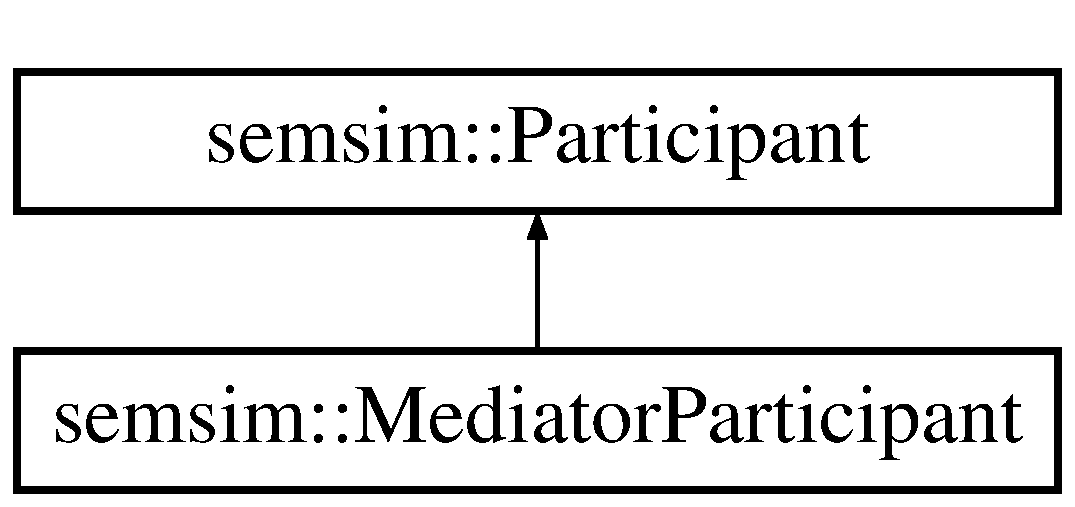
\includegraphics[height=2.000000cm]{classsemsim_1_1MediatorParticipant}
                                                              \end{center}
\end{figure}
\doxysubsection*{Public Member Functions}
\begin{DoxyCompactItemize}
    \item
    \mbox{\Hypertarget{classsemsim_1_1MediatorParticipant_a068e325880c96b598b5ea87edcaffcd4}\label{classsemsim_1_1MediatorParticipant_a068e325880c96b598b5ea87edcaffcd4}}
    {\bfseries Mediator\+Participant} (Librdf\+World world, Librdf\+Model model, std\+::string subject, std\+::string physical\+Entity\+Reference)
\end{DoxyCompactItemize}


The documentation for this class was generated from the following files\+:\begin{DoxyCompactItemize}
                                                                              \item
                                                                              src/semsim/Participant.\+h\item
                                                                              src/semsim/Participant.\+cpp
\end{DoxyCompactItemize}

\hypertarget{classsemsim_1_1MetaID}{}\section{semsim\+:\+:Meta\+ID Class Reference}
\label{classsemsim_1_1MetaID}\index{semsim\+::\+Meta\+ID@{semsim\+::\+Meta\+ID}}
\subsection*{Public Member Functions}
\begin{DoxyCompactItemize}
\item 
\mbox{\Hypertarget{classsemsim_1_1MetaID_a63833c9ae3303f451181f9d118c0d51c}\label{classsemsim_1_1MetaID_a63833c9ae3303f451181f9d118c0d51c}} 
{\bfseries Meta\+ID} (std\+::string base, long number, int num\+\_\+digits=4)
\item 
\mbox{\Hypertarget{classsemsim_1_1MetaID_a4b39fce25e5db81fdd59cfbc4f4734da}\label{classsemsim_1_1MetaID_a4b39fce25e5db81fdd59cfbc4f4734da}} 
bool {\bfseries operator==} (const \hyperlink{classsemsim_1_1MetaID}{Meta\+ID} \&rhs) const
\item 
\mbox{\Hypertarget{classsemsim_1_1MetaID_a128d53d2d266cf1f88ef13ee9c21a2c0}\label{classsemsim_1_1MetaID_a128d53d2d266cf1f88ef13ee9c21a2c0}} 
bool {\bfseries operator!=} (const \hyperlink{classsemsim_1_1MetaID}{Meta\+ID} \&rhs) const
\item 
\mbox{\Hypertarget{classsemsim_1_1MetaID_aefd0d224e3930da32f927a4ff8c8bc74}\label{classsemsim_1_1MetaID_aefd0d224e3930da32f927a4ff8c8bc74}} 
std\+::string {\bfseries generate} () const
\item 
\mbox{\Hypertarget{classsemsim_1_1MetaID_a6336339cef2d12f7eea49bab94e45171}\label{classsemsim_1_1MetaID_a6336339cef2d12f7eea49bab94e45171}} 
std\+::string {\bfseries generate} (long n) const
\item 
\mbox{\Hypertarget{classsemsim_1_1MetaID_a2a9408d835ed445a90b43843404e9fbe}\label{classsemsim_1_1MetaID_a2a9408d835ed445a90b43843404e9fbe}} 
int {\bfseries max\+Number} () const
\end{DoxyCompactItemize}
\subsection*{Static Public Member Functions}
\begin{DoxyCompactItemize}
\item 
\mbox{\Hypertarget{classsemsim_1_1MetaID_aa4f326f8b965d3dd7af038793e7806ad}\label{classsemsim_1_1MetaID_aa4f326f8b965d3dd7af038793e7806ad}} 
static int {\bfseries count\+Digits} (long n)
\end{DoxyCompactItemize}


The documentation for this class was generated from the following files\+:\begin{DoxyCompactItemize}
\item 
src/semsim/Meta\+I\+D.\+h\item 
src/semsim/Meta\+I\+D.\+cpp\end{DoxyCompactItemize}

\hypertarget{classsemsim_1_1NotImplementedException}{}\doxysection{semsim\+::Not\+Implemented\+Exception Class Reference}
\label{classsemsim_1_1NotImplementedException}\index{semsim::NotImplementedException@{semsim::NotImplementedException}}
Inheritance diagram for semsim\+::Not\+Implemented\+Exception\+:\begin{figure}[H]
                                                                    \begin{center}
                                                                        \leavevmode
                                                                        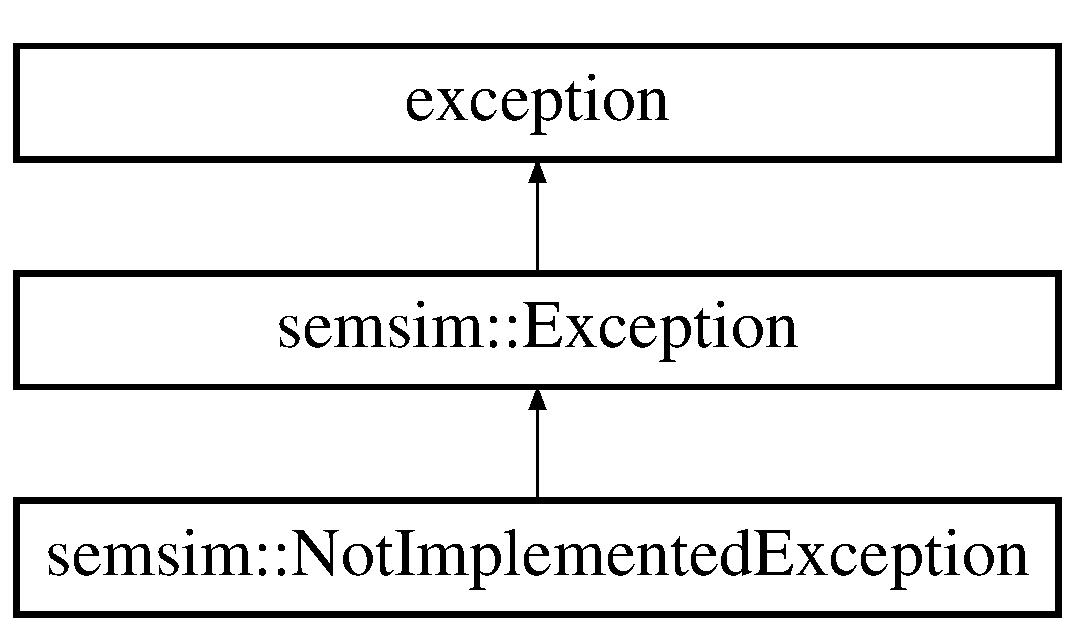
\includegraphics[height=3.000000cm]{classsemsim_1_1NotImplementedException}
                                                                    \end{center}
\end{figure}
\doxysubsection*{Additional Inherited Members}


The documentation for this class was generated from the following file\+:\begin{DoxyCompactItemize}
                                                                             \item
                                                                             src/semsim/Error.\+h
\end{DoxyCompactItemize}

\hypertarget{classsemsim_1_1NullPointerException}{}\section{semsim\+:\+:Null\+Pointer\+Exception Class Reference}
\label{classsemsim_1_1NullPointerException}\index{semsim\+::\+Null\+Pointer\+Exception@{semsim\+::\+Null\+Pointer\+Exception}}
Inheritance diagram for semsim\+:\+:Null\+Pointer\+Exception\+:\begin{figure}[H]
\begin{center}
\leavevmode
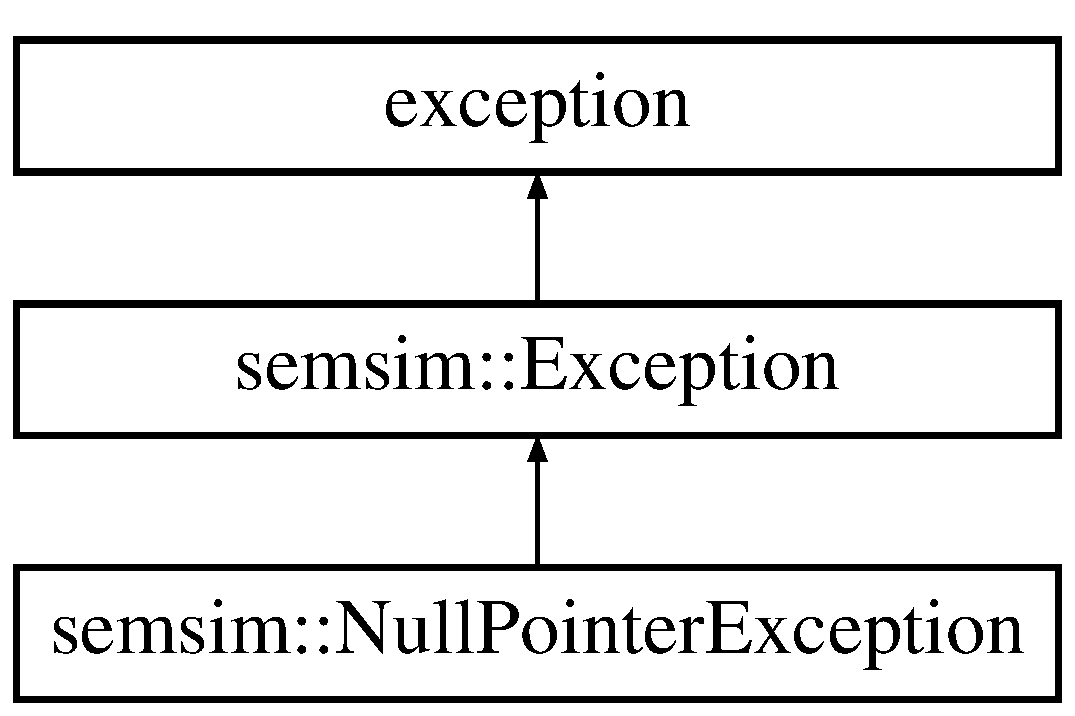
\includegraphics[height=3.000000cm]{classsemsim_1_1NullPointerException}
\end{center}
\end{figure}
\subsection*{Additional Inherited Members}


The documentation for this class was generated from the following file\+:\begin{DoxyCompactItemize}
\item 
src/semsim/Error.\+h\end{DoxyCompactItemize}

\hypertarget{classsemsim_1_1Participant}{}\section{semsim\+:\+:Participant Class Reference}
\label{classsemsim_1_1Participant}\index{semsim\+::\+Participant@{semsim\+::\+Participant}}
Inheritance diagram for semsim\+:\+:Participant\+:\begin{figure}[H]
\begin{center}
\leavevmode
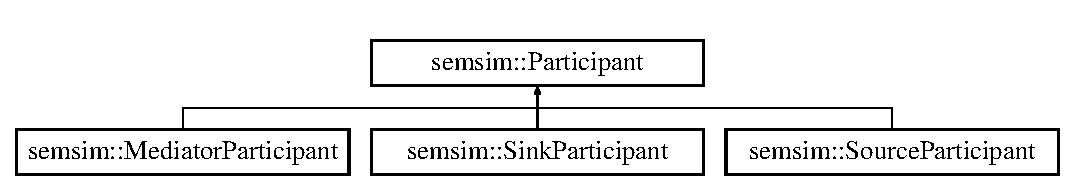
\includegraphics[height=2.000000cm]{classsemsim_1_1Participant}
\end{center}
\end{figure}
\subsection*{Public Member Functions}
\begin{DoxyCompactItemize}
\item 
\mbox{\Hypertarget{classsemsim_1_1Participant_a7ff795c36df78aab96143b41ae91bbc2}\label{classsemsim_1_1Participant_a7ff795c36df78aab96143b41ae91bbc2}} 
void {\bfseries free} ()
\item 
\mbox{\Hypertarget{classsemsim_1_1Participant_aae54a8e515392c073a65bf6cb0915656}\label{classsemsim_1_1Participant_aae54a8e515392c073a65bf6cb0915656}} 
{\bfseries Participant} (librdf\+\_\+model $\ast$model, std\+::string subject, std\+::string semsim\+\_\+predicate\+\_\+term, double multiplier, std\+::string physical\+Entity\+Reference)
\item 
\mbox{\Hypertarget{classsemsim_1_1Participant_a0713dcb34036f27f80ff2551b979add4}\label{classsemsim_1_1Participant_a0713dcb34036f27f80ff2551b979add4}} 
\hyperlink{classsemsim_1_1Triples}{Triples} {\bfseries to\+Triples} (const std\+::string \&process\+\_\+metaid) const
\item 
\mbox{\Hypertarget{classsemsim_1_1Participant_a0d3d2dbb034cad4729312cae8ecf81d8}\label{classsemsim_1_1Participant_a0d3d2dbb034cad4729312cae8ecf81d8}} 
\hyperlink{classsemsim_1_1SemSim}{Sem\+Sim} {\bfseries get\+Predicate} ()
\item 
\mbox{\Hypertarget{classsemsim_1_1Participant_a01b7a448760d6e8a088adef0efe9964a}\label{classsemsim_1_1Participant_a01b7a448760d6e8a088adef0efe9964a}} 
void {\bfseries set\+Predicate} (std\+::string semsim\+\_\+predicate\+\_\+string)
\item 
\mbox{\Hypertarget{classsemsim_1_1Participant_acfdc8056b288b3e36d54248d03d96c5c}\label{classsemsim_1_1Participant_acfdc8056b288b3e36d54248d03d96c5c}} 
const std\+::string \& {\bfseries get\+Subject} () const
\item 
\mbox{\Hypertarget{classsemsim_1_1Participant_aca088588f5fa41042be8cc43ceeb7962}\label{classsemsim_1_1Participant_aca088588f5fa41042be8cc43ceeb7962}} 
double {\bfseries get\+Multiplier} () const
\item 
\mbox{\Hypertarget{classsemsim_1_1Participant_a7c9e14ea7bc01d2fc6b655a990b370f3}\label{classsemsim_1_1Participant_a7c9e14ea7bc01d2fc6b655a990b370f3}} 
const std\+::string \& {\bfseries get\+Physical\+Entity\+Reference} () const
\end{DoxyCompactItemize}


The documentation for this class was generated from the following files\+:\begin{DoxyCompactItemize}
\item 
src/semsim/Participant.\+h\item 
src/semsim/Participant.\+cpp\end{DoxyCompactItemize}

\hypertarget{classsemsim_1_1PhysicalEntity}{}\section{semsim\+:\+:Physical\+Entity Class Reference}
\label{classsemsim_1_1PhysicalEntity}\index{semsim\+::\+Physical\+Entity@{semsim\+::\+Physical\+Entity}}
Inheritance diagram for semsim\+:\+:Physical\+Entity\+:\begin{figure}[H]
\begin{center}
\leavevmode
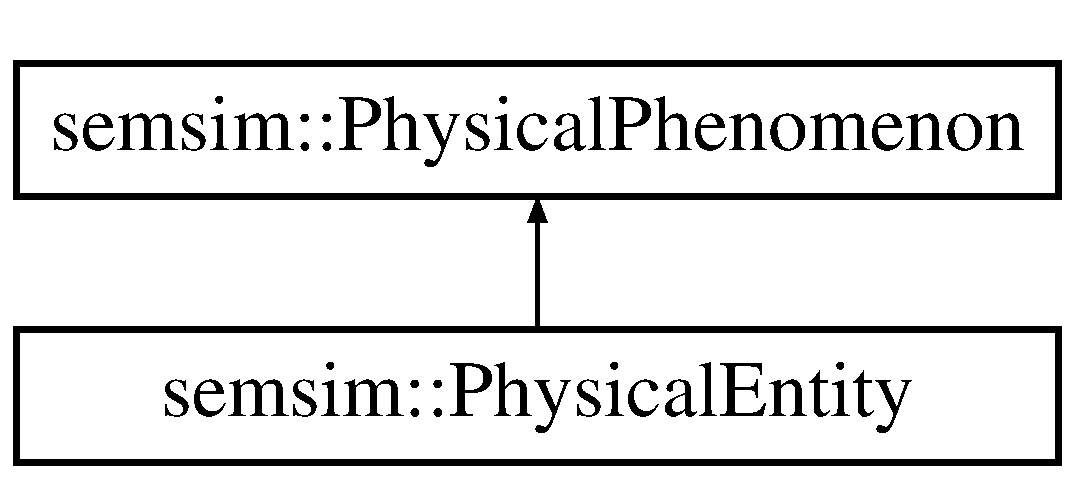
\includegraphics[height=2.000000cm]{classsemsim_1_1PhysicalEntity}
\end{center}
\end{figure}
\subsection*{Public Member Functions}
\begin{DoxyCompactItemize}
\item 
\mbox{\Hypertarget{classsemsim_1_1PhysicalEntity_a38bf3915fbd86b2adb9e9779301a94b3}\label{classsemsim_1_1PhysicalEntity_a38bf3915fbd86b2adb9e9779301a94b3}} 
{\bfseries Physical\+Entity} (librdf\+\_\+model $\ast$model, \hyperlink{classsemsim_1_1Subject}{Subject} about, \hyperlink{classsemsim_1_1PhysicalPropertyResource}{Physical\+Property\+Resource} physical\+Property, \hyperlink{classsemsim_1_1Resource}{Resource} is, Resources is\+\_\+part\+\_\+of)
\item 
\mbox{\Hypertarget{classsemsim_1_1PhysicalEntity_a3978fc7ce8633d583965a858ee99a418}\label{classsemsim_1_1PhysicalEntity_a3978fc7ce8633d583965a858ee99a418}} 
void {\bfseries free} () override
\item 
\mbox{\Hypertarget{classsemsim_1_1PhysicalEntity_a1df028fe0ee3f7f58e2eb7ea28d118ec}\label{classsemsim_1_1PhysicalEntity_a1df028fe0ee3f7f58e2eb7ea28d118ec}} 
{\bfseries Physical\+Entity} (librdf\+\_\+model $\ast$model)
\item 
\mbox{\Hypertarget{classsemsim_1_1PhysicalEntity_a32f4240e1ab47f422e704f97c669e824}\label{classsemsim_1_1PhysicalEntity_a32f4240e1ab47f422e704f97c669e824}} 
\hyperlink{classsemsim_1_1Triples}{Triples} {\bfseries to\+Triples} () override
\item 
\mbox{\Hypertarget{classsemsim_1_1PhysicalEntity_a5940a4984dbd8fb6cef55de5cd36a9b4}\label{classsemsim_1_1PhysicalEntity_a5940a4984dbd8fb6cef55de5cd36a9b4}} 
const \hyperlink{classsemsim_1_1Resource}{Resource} \& {\bfseries get\+Identity\+Resource} () const
\item 
\mbox{\Hypertarget{classsemsim_1_1PhysicalEntity_aa2aeec22fc0f703b2e83fcfd59b25f29}\label{classsemsim_1_1PhysicalEntity_aa2aeec22fc0f703b2e83fcfd59b25f29}} 
const Resources \& {\bfseries get\+Location\+Resources} () const
\item 
\mbox{\Hypertarget{classsemsim_1_1PhysicalEntity_aa5b88988a264a59b174452ec49f824ba}\label{classsemsim_1_1PhysicalEntity_aa5b88988a264a59b174452ec49f824ba}} 
\hyperlink{classsemsim_1_1PhysicalEntity}{Physical\+Entity} \& {\bfseries set\+About} (std\+::string metaid)
\item 
\mbox{\Hypertarget{classsemsim_1_1PhysicalEntity_ae2408ca531d0755ff28ad1e4f062023d}\label{classsemsim_1_1PhysicalEntity_ae2408ca531d0755ff28ad1e4f062023d}} 
\hyperlink{classsemsim_1_1PhysicalEntity}{Physical\+Entity} \& {\bfseries set\+Physical\+Property} (const std\+::string \&physical\+Property)
\item 
\mbox{\Hypertarget{classsemsim_1_1PhysicalEntity_a4aa4c32d99568eb43ec97d8371ded354}\label{classsemsim_1_1PhysicalEntity_a4aa4c32d99568eb43ec97d8371ded354}} 
\hyperlink{classsemsim_1_1PhysicalEntity}{Physical\+Entity} \& {\bfseries set\+Physical\+Property} (\hyperlink{classsemsim_1_1PhysicalPropertyResource}{Physical\+Property\+Resource} physical\+Property)
\item 
\mbox{\Hypertarget{classsemsim_1_1PhysicalEntity_ab3e7a2142a90e18150323268acc92217}\label{classsemsim_1_1PhysicalEntity_ab3e7a2142a90e18150323268acc92217}} 
\hyperlink{classsemsim_1_1PhysicalEntity}{Physical\+Entity} \& {\bfseries set\+Identity} (std\+::string resource)
\item 
\mbox{\Hypertarget{classsemsim_1_1PhysicalEntity_a1b35c526b4265b920d9d483842e0150d}\label{classsemsim_1_1PhysicalEntity_a1b35c526b4265b920d9d483842e0150d}} 
\hyperlink{classsemsim_1_1PhysicalEntity}{Physical\+Entity} \& {\bfseries add\+Location} (std\+::string where)
\item 
\mbox{\Hypertarget{classsemsim_1_1PhysicalEntity_a8db27f0206e3d827f5b8866459a771aa}\label{classsemsim_1_1PhysicalEntity_a8db27f0206e3d827f5b8866459a771aa}} 
int {\bfseries get\+Num\+Locations} () const
\end{DoxyCompactItemize}
\subsection*{Additional Inherited Members}


The documentation for this class was generated from the following files\+:\begin{DoxyCompactItemize}
\item 
src/semsim/Physical\+Entity.\+h\item 
src/semsim/Physical\+Entity.\+cpp\end{DoxyCompactItemize}

\hypertarget{classsemsim_1_1PhysicalForce}{}\section{semsim\+:\+:Physical\+Force Class Reference}
\label{classsemsim_1_1PhysicalForce}\index{semsim\+::\+Physical\+Force@{semsim\+::\+Physical\+Force}}
Inheritance diagram for semsim\+:\+:Physical\+Force\+:\begin{figure}[H]
\begin{center}
\leavevmode
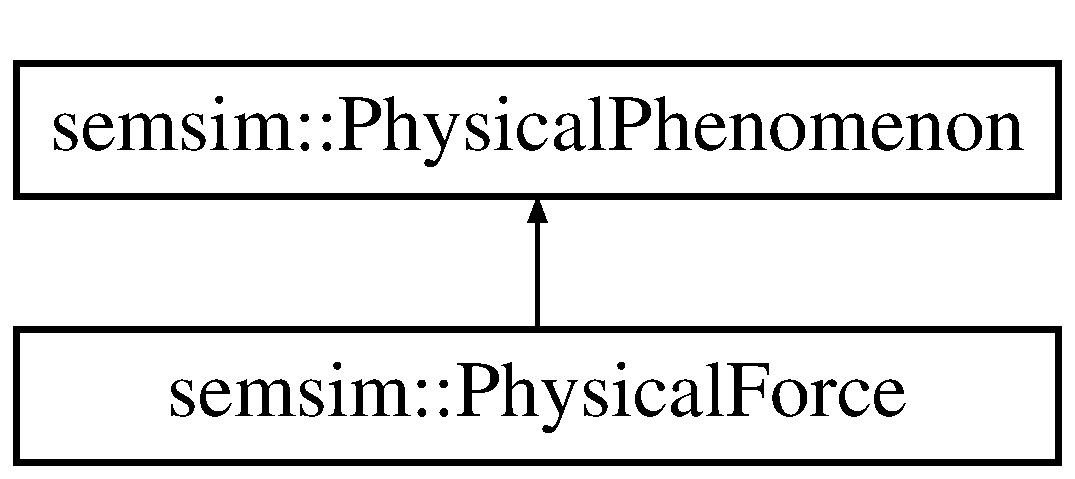
\includegraphics[height=2.000000cm]{classsemsim_1_1PhysicalForce}
\end{center}
\end{figure}
\subsection*{Public Member Functions}
\begin{DoxyCompactItemize}
\item 
\mbox{\Hypertarget{classsemsim_1_1PhysicalForce_ab4a55fec692b38b868ddd357f82969bd}\label{classsemsim_1_1PhysicalForce_ab4a55fec692b38b868ddd357f82969bd}} 
{\bfseries Physical\+Force} (librdf\+\_\+model $\ast$model, \hyperlink{classsemsim_1_1Subject}{Subject} metaid, \hyperlink{classsemsim_1_1PhysicalPropertyResource}{Physical\+Property\+Resource} physical\+Property, Sources sources, Sinks sinks)
\item 
\mbox{\Hypertarget{classsemsim_1_1PhysicalForce_a5d5a07e0f6d88cd5569c78a6039f3de1}\label{classsemsim_1_1PhysicalForce_a5d5a07e0f6d88cd5569c78a6039f3de1}} 
void {\bfseries free} () override
\item 
\mbox{\Hypertarget{classsemsim_1_1PhysicalForce_a08cf520fbe7955eca7766b9d2c5bc0c8}\label{classsemsim_1_1PhysicalForce_a08cf520fbe7955eca7766b9d2c5bc0c8}} 
{\bfseries Physical\+Force} (librdf\+\_\+model $\ast$model)
\item 
\mbox{\Hypertarget{classsemsim_1_1PhysicalForce_a740ffadd18b39ce922b41633db3e24af}\label{classsemsim_1_1PhysicalForce_a740ffadd18b39ce922b41633db3e24af}} 
std\+::string {\bfseries create\+Meta\+Id} () const
\item 
\mbox{\Hypertarget{classsemsim_1_1PhysicalForce_a3641e487b723088a5ecf82488877cc34}\label{classsemsim_1_1PhysicalForce_a3641e487b723088a5ecf82488877cc34}} 
const Sources \& {\bfseries get\+Sources} () const
\item 
\mbox{\Hypertarget{classsemsim_1_1PhysicalForce_a5ca80b2444abf551937c7864abea4980}\label{classsemsim_1_1PhysicalForce_a5ca80b2444abf551937c7864abea4980}} 
const Sinks \& {\bfseries get\+Sinks} () const
\item 
\mbox{\Hypertarget{classsemsim_1_1PhysicalForce_a9b8be504b403b781a34ca5df9c3bbc2d}\label{classsemsim_1_1PhysicalForce_a9b8be504b403b781a34ca5df9c3bbc2d}} 
\hyperlink{classsemsim_1_1Triples}{Triples} {\bfseries to\+Triples} () override
\item 
\mbox{\Hypertarget{classsemsim_1_1PhysicalForce_ad817f08d345b53a2e7fb80052457f8c8}\label{classsemsim_1_1PhysicalForce_ad817f08d345b53a2e7fb80052457f8c8}} 
\hyperlink{classsemsim_1_1PhysicalForce}{Physical\+Force} \& {\bfseries set\+About} (const std\+::string \&metaid)
\item 
\mbox{\Hypertarget{classsemsim_1_1PhysicalForce_a5a83ae2458a89151ed7990ba75251318}\label{classsemsim_1_1PhysicalForce_a5a83ae2458a89151ed7990ba75251318}} 
\hyperlink{classsemsim_1_1PhysicalForce}{Physical\+Force} \& {\bfseries set\+Physical\+Property} (\hyperlink{classsemsim_1_1PhysicalPropertyResource}{Physical\+Property\+Resource} physical\+Property)
\item 
\mbox{\Hypertarget{classsemsim_1_1PhysicalForce_a684767a1350eab54b403c5b1dd0cb20a}\label{classsemsim_1_1PhysicalForce_a684767a1350eab54b403c5b1dd0cb20a}} 
\hyperlink{classsemsim_1_1PhysicalForce}{Physical\+Force} \& {\bfseries set\+Physical\+Property} (const std\+::string \&physical\+Property)
\item 
\mbox{\Hypertarget{classsemsim_1_1PhysicalForce_afe234b09ac757b4cf3561f8d3cbf4c0b}\label{classsemsim_1_1PhysicalForce_afe234b09ac757b4cf3561f8d3cbf4c0b}} 
\hyperlink{classsemsim_1_1PhysicalForce}{Physical\+Force} \& {\bfseries add\+Source} (std\+::string source\+\_\+metaid, double multiplier, std\+::string physical\+\_\+entity\+\_\+reference)
\item 
\mbox{\Hypertarget{classsemsim_1_1PhysicalForce_a0886647a9a7efd80bb99f6ce74bcb76a}\label{classsemsim_1_1PhysicalForce_a0886647a9a7efd80bb99f6ce74bcb76a}} 
\hyperlink{classsemsim_1_1PhysicalForce}{Physical\+Force} \& {\bfseries add\+Sink} (std\+::string sink\+\_\+metaid, double multiplier, std\+::string physical\+\_\+entity\+\_\+reference)
\item 
\mbox{\Hypertarget{classsemsim_1_1PhysicalForce_ad94974c799d17e5f6376391b1f3a7444}\label{classsemsim_1_1PhysicalForce_ad94974c799d17e5f6376391b1f3a7444}} 
int {\bfseries get\+Num\+Sources} ()
\item 
\mbox{\Hypertarget{classsemsim_1_1PhysicalForce_ab947284af190941616ae8a6f1de2a85d}\label{classsemsim_1_1PhysicalForce_ab947284af190941616ae8a6f1de2a85d}} 
int {\bfseries get\+Num\+Sinks} ()
\end{DoxyCompactItemize}
\subsection*{Additional Inherited Members}


The documentation for this class was generated from the following files\+:\begin{DoxyCompactItemize}
\item 
src/semsim/Physical\+Force.\+h\item 
src/semsim/Physical\+Force.\+cpp\end{DoxyCompactItemize}

\hypertarget{classsemsim_1_1PhysicalPhenomenon}{}\doxysection{semsim\+::Physical\+Phenomenon Class Reference}
\label{classsemsim_1_1PhysicalPhenomenon}\index{semsim::PhysicalPhenomenon@{semsim::PhysicalPhenomenon}}
Inheritance diagram for semsim\+::Physical\+Phenomenon\+:\begin{figure}[H]
                                                             \begin{center}
                                                                 \leavevmode
                                                                 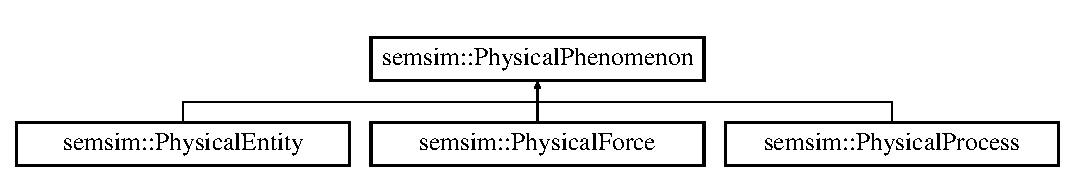
\includegraphics[height=1.996435cm]{classsemsim_1_1PhysicalPhenomenon}
                                                             \end{center}
\end{figure}
\doxysubsection*{Public Member Functions}
\begin{DoxyCompactItemize}
    \item
    \mbox{\Hypertarget{classsemsim_1_1PhysicalPhenomenon_a4923938fde324d41d9d2d171c380d512}\label{classsemsim_1_1PhysicalPhenomenon_a4923938fde324d41d9d2d171c380d512}}
    {\bfseries Physical\+Phenomenon} (Librdf\+World world, Librdf\+Model model, \mbox{\hyperlink{classsemsim_1_1Subject}{Subject}} metaid, \mbox{\hyperlink{classsemsim_1_1PhysicalPropertyResource}{Physical\+Property\+Resource}} property\+Resource, Annotation\+Type type)
    \item
    \mbox{\Hypertarget{classsemsim_1_1PhysicalPhenomenon_a7d148d741a60a8384e596b9902d5675d}\label{classsemsim_1_1PhysicalPhenomenon_a7d148d741a60a8384e596b9902d5675d}}
    {\bfseries Physical\+Phenomenon} (Librdf\+World world, Librdf\+Model model)
    \item
    \mbox{\Hypertarget{classsemsim_1_1PhysicalPhenomenon_af3a680b3bacba8733eab51207fa8e223}\label{classsemsim_1_1PhysicalPhenomenon_af3a680b3bacba8733eab51207fa8e223}}
    \mbox{\hyperlink{classsemsim_1_1Subject}{Subject}} {\bfseries get\+About} () const
    \item
    \mbox{\Hypertarget{classsemsim_1_1PhysicalPhenomenon_ae56630b175214b2196da1bf47a3c47c0}\label{classsemsim_1_1PhysicalPhenomenon_ae56630b175214b2196da1bf47a3c47c0}}
    \mbox{\hyperlink{classsemsim_1_1Subject}{Subject}} {\bfseries get\+Subject} () const
    \item
    \mbox{\Hypertarget{classsemsim_1_1PhysicalPhenomenon_a3fc27dfe9bedd3055c575e134c537d6e}\label{classsemsim_1_1PhysicalPhenomenon_a3fc27dfe9bedd3055c575e134c537d6e}}
    Annotation\+Type {\bfseries get\+Type} () const
    \item
    \mbox{\Hypertarget{classsemsim_1_1PhysicalPhenomenon_ac0b9bb899a6bd02275b5b4d106f875ea}\label{classsemsim_1_1PhysicalPhenomenon_ac0b9bb899a6bd02275b5b4d106f875ea}}
    \mbox{\hyperlink{classsemsim_1_1PhysicalPropertyResource}{Physical\+Property\+Resource}} {\bfseries get\+Physical\+Property} () const
    \item
    \mbox{\Hypertarget{classsemsim_1_1PhysicalPhenomenon_a1856c2c2c86e053d8b164f401810f308}\label{classsemsim_1_1PhysicalPhenomenon_a1856c2c2c86e053d8b164f401810f308}}
    virtual \mbox{\hyperlink{classsemsim_1_1Triples}{Triples}} {\bfseries to\+Triples} () const
\end{DoxyCompactItemize}
\doxysubsection*{Protected Member Functions}
\begin{DoxyCompactItemize}
    \item
    \mbox{\Hypertarget{classsemsim_1_1PhysicalPhenomenon_a930e9d0f75ec3a7bdbcb2dbce1a47716}\label{classsemsim_1_1PhysicalPhenomenon_a930e9d0f75ec3a7bdbcb2dbce1a47716}}
    std\+::string {\bfseries generate\+Meta\+Id} (std\+::string id\+\_\+base) const
\end{DoxyCompactItemize}
\doxysubsection*{Protected Attributes}
\begin{DoxyCompactItemize}
    \item
    \mbox{\Hypertarget{classsemsim_1_1PhysicalPhenomenon_a6352d5bc90b9050b6b8eda6f5691d0a3}\label{classsemsim_1_1PhysicalPhenomenon_a6352d5bc90b9050b6b8eda6f5691d0a3}}
    Librdf\+World {\bfseries world\+\_\+}
    \item
    \mbox{\Hypertarget{classsemsim_1_1PhysicalPhenomenon_ae90491b509bf2c7d7b604804fc1b34e5}\label{classsemsim_1_1PhysicalPhenomenon_ae90491b509bf2c7d7b604804fc1b34e5}}
    Librdf\+Model {\bfseries model\+\_\+}
    \item
    \mbox{\Hypertarget{classsemsim_1_1PhysicalPhenomenon_aa43a5f6719a6d44d4b96081b2f2622fe}\label{classsemsim_1_1PhysicalPhenomenon_aa43a5f6719a6d44d4b96081b2f2622fe}}
    \mbox{\hyperlink{classsemsim_1_1Subject}{Subject}} {\bfseries about}
    \item
    \mbox{\Hypertarget{classsemsim_1_1PhysicalPhenomenon_a264d752c356d2c6011da6d3cd1494418}\label{classsemsim_1_1PhysicalPhenomenon_a264d752c356d2c6011da6d3cd1494418}}
    \mbox{\hyperlink{classsemsim_1_1PhysicalPropertyResource}{Physical\+Property\+Resource}} {\bfseries physical\+\_\+property\+\_\+}
    \item
    \mbox{\Hypertarget{classsemsim_1_1PhysicalPhenomenon_ad18e38168bcec1925e6bd9ed08494614}\label{classsemsim_1_1PhysicalPhenomenon_ad18e38168bcec1925e6bd9ed08494614}}
    Annotation\+Type {\bfseries type\+\_\+}
\end{DoxyCompactItemize}


The documentation for this class was generated from the following files\+:\begin{DoxyCompactItemize}
                                                                              \item
                                                                              src/semsim/Physical\+Phenomenon.\+h\item
                                                                              src/semsim/Physical\+Phenomenon.\+cpp
\end{DoxyCompactItemize}

\hypertarget{classsemsim_1_1PhysicalProcess}{}\doxysection{semsim\+::Physical\+Process Class Reference}
\label{classsemsim_1_1PhysicalProcess}\index{semsim::PhysicalProcess@{semsim::PhysicalProcess}}
Inheritance diagram for semsim\+::Physical\+Process\+:\begin{figure}[H]
                                                          \begin{center}
                                                              \leavevmode
                                                              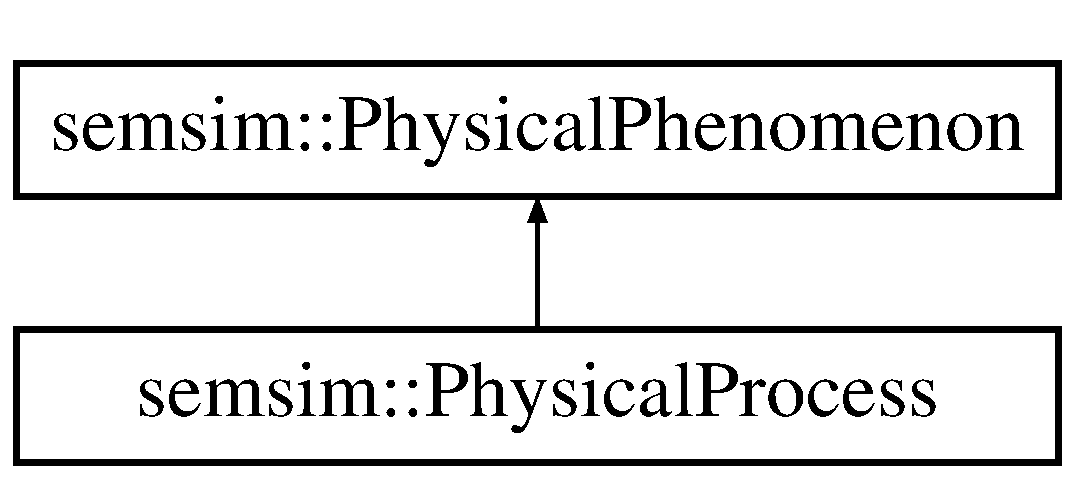
\includegraphics[height=2.000000cm]{classsemsim_1_1PhysicalProcess}
                                                          \end{center}
\end{figure}
\doxysubsection*{Public Member Functions}
\begin{DoxyCompactItemize}
    \item
    \mbox{\Hypertarget{classsemsim_1_1PhysicalProcess_af1c08533ad511aacbd2f69516b297ed2}\label{classsemsim_1_1PhysicalProcess_af1c08533ad511aacbd2f69516b297ed2}}
    {\bfseries Physical\+Process} (Librdf\+World world, Librdf\+Model model, \mbox{\hyperlink{classsemsim_1_1Subject}{Subject}} metaid, \mbox{\hyperlink{classsemsim_1_1PhysicalPropertyResource}{Physical\+Property\+Resource}} physical\+Property, Sources sources, Sinks sinks, Mediators mediators)
    \item
    \mbox{\Hypertarget{classsemsim_1_1PhysicalProcess_a68b08a9ac105bb5e946c2db77125b557}\label{classsemsim_1_1PhysicalProcess_a68b08a9ac105bb5e946c2db77125b557}}
    {\bfseries Physical\+Process} (Librdf\+World world, Librdf\+Model model)
    \item
    \mbox{\Hypertarget{classsemsim_1_1PhysicalProcess_a6d3ea622c0f1fa642068b1b7e76385e5}\label{classsemsim_1_1PhysicalProcess_a6d3ea622c0f1fa642068b1b7e76385e5}}
    const Sources \& {\bfseries get\+Sources} () const
    \item
    \mbox{\Hypertarget{classsemsim_1_1PhysicalProcess_aa7ec750398cf738c374c9e92c0bb5670}\label{classsemsim_1_1PhysicalProcess_aa7ec750398cf738c374c9e92c0bb5670}}
    const Sinks \& {\bfseries get\+Sinks} () const
    \item
    \mbox{\Hypertarget{classsemsim_1_1PhysicalProcess_a127806bf74ec1e31514c6f3d659824b3}\label{classsemsim_1_1PhysicalProcess_a127806bf74ec1e31514c6f3d659824b3}}
    const Mediators \& {\bfseries get\+Mediators} () const
    \item
    \mbox{\Hypertarget{classsemsim_1_1PhysicalProcess_a45383f5e8d1403cdb314795062d4a35a}\label{classsemsim_1_1PhysicalProcess_a45383f5e8d1403cdb314795062d4a35a}}
    \mbox{\hyperlink{classsemsim_1_1Triples}{Triples}} {\bfseries to\+Triples} () const override
    \item
    \mbox{\Hypertarget{classsemsim_1_1PhysicalProcess_a1caf11364214c1f0e379729e92333208}\label{classsemsim_1_1PhysicalProcess_a1caf11364214c1f0e379729e92333208}}
    \mbox{\hyperlink{classsemsim_1_1PhysicalProcess}{Physical\+Process}} \& {\bfseries set\+About} (std\+::string metaid)
    \item
    \mbox{\Hypertarget{classsemsim_1_1PhysicalProcess_ad5015bd89fef10553e03f0f6b4b13085}\label{classsemsim_1_1PhysicalProcess_ad5015bd89fef10553e03f0f6b4b13085}}
    \mbox{\hyperlink{classsemsim_1_1PhysicalProcess}{Physical\+Process}} \& {\bfseries set\+Physical\+Property} (\mbox{\hyperlink{classsemsim_1_1PhysicalPropertyResource}{Physical\+Property\+Resource}} physical\+Property)
    \item
    \mbox{\Hypertarget{classsemsim_1_1PhysicalProcess_a28eeb2d8344664a842b725249bea7dec}\label{classsemsim_1_1PhysicalProcess_a28eeb2d8344664a842b725249bea7dec}}
    \mbox{\hyperlink{classsemsim_1_1PhysicalProcess}{Physical\+Process}} \& {\bfseries add\+Source} (std\+::string source\+\_\+metaid, double multiplier, std\+::string physical\+\_\+entity\+\_\+reference)
    \item
    \mbox{\Hypertarget{classsemsim_1_1PhysicalProcess_a88c77abfb77d9a006da62fd0c0730007}\label{classsemsim_1_1PhysicalProcess_a88c77abfb77d9a006da62fd0c0730007}}
    \mbox{\hyperlink{classsemsim_1_1PhysicalProcess}{Physical\+Process}} \& {\bfseries add\+Sink} (std\+::string sink\+\_\+metaid, double multiplier, std\+::string physical\+\_\+entity\+\_\+reference)
    \item
    \mbox{\Hypertarget{classsemsim_1_1PhysicalProcess_a798bda68e6b2fb7940e3400b003c1d7d}\label{classsemsim_1_1PhysicalProcess_a798bda68e6b2fb7940e3400b003c1d7d}}
    \mbox{\hyperlink{classsemsim_1_1PhysicalProcess}{Physical\+Process}} \& {\bfseries add\+Mediator} (std\+::string mediator\+\_\+metaid, double multiplier, std\+::string physical\+\_\+entity\+\_\+reference)
    \item
    \mbox{\Hypertarget{classsemsim_1_1PhysicalProcess_a5b0b6e6d5eba493fed10759497057f1b}\label{classsemsim_1_1PhysicalProcess_a5b0b6e6d5eba493fed10759497057f1b}}
    \mbox{\hyperlink{classsemsim_1_1PhysicalProcess}{Physical\+Process}} \& {\bfseries set\+Physical\+Property} (const std\+::string \&physical\+Property)
    \item
    \mbox{\Hypertarget{classsemsim_1_1PhysicalProcess_a07fa014685889073952834086b3a74a4}\label{classsemsim_1_1PhysicalProcess_a07fa014685889073952834086b3a74a4}}
    int {\bfseries get\+Num\+Sources} ()
    \item
    \mbox{\Hypertarget{classsemsim_1_1PhysicalProcess_a66d037746715d730964329cccc5e68ba}\label{classsemsim_1_1PhysicalProcess_a66d037746715d730964329cccc5e68ba}}
    int {\bfseries get\+Num\+Sinks} ()
    \item
    \mbox{\Hypertarget{classsemsim_1_1PhysicalProcess_a6223cd90d08c19c4c81f4c72ffb1379b}\label{classsemsim_1_1PhysicalProcess_a6223cd90d08c19c4c81f4c72ffb1379b}}
    int {\bfseries get\+Num\+Mediators} ()
\end{DoxyCompactItemize}
\doxysubsection*{Additional Inherited Members}


The documentation for this class was generated from the following files\+:\begin{DoxyCompactItemize}
                                                                              \item
                                                                              src/semsim/Physical\+Process.\+h\item
                                                                              src/semsim/Physical\+Process.\+cpp
\end{DoxyCompactItemize}

\hypertarget{classsemsim_1_1PhysicalPropertyResource}{}\section{semsim\+:\+:Physical\+Property\+Resource Class Reference}
\label{classsemsim_1_1PhysicalPropertyResource}\index{semsim\+::\+Physical\+Property\+Resource@{semsim\+::\+Physical\+Property\+Resource}}
Inheritance diagram for semsim\+:\+:Physical\+Property\+Resource\+:\begin{figure}[H]
\begin{center}
\leavevmode
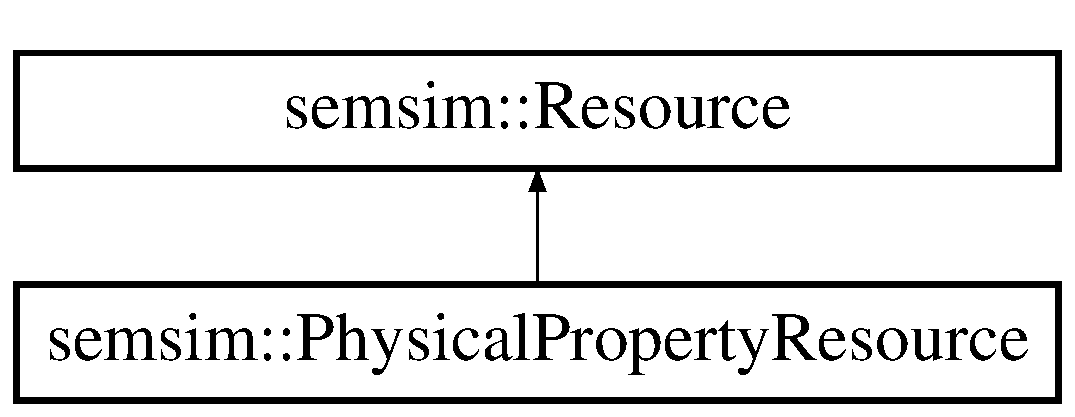
\includegraphics[height=2.000000cm]{classsemsim_1_1PhysicalPropertyResource}
\end{center}
\end{figure}
\subsection*{Public Member Functions}
\begin{DoxyCompactItemize}
\item 
\mbox{\Hypertarget{classsemsim_1_1PhysicalPropertyResource_aa1fd98e8e7f451f7e399f4eed1b66521}\label{classsemsim_1_1PhysicalPropertyResource_aa1fd98e8e7f451f7e399f4eed1b66521}} 
{\bfseries Physical\+Property\+Resource} (std\+::string physical\+\_\+property\+\_\+string)
\item 
\mbox{\Hypertarget{classsemsim_1_1PhysicalPropertyResource_a2368cabb4268b7869dc550caca498d36}\label{classsemsim_1_1PhysicalPropertyResource_a2368cabb4268b7869dc550caca498d36}} 
\hyperlink{classsemsim_1_1Triple}{Triple} {\bfseries is\+Version\+Of\+Triple} (std\+::string subject\+\_\+metaid) const
\item 
\mbox{\Hypertarget{classsemsim_1_1PhysicalPropertyResource_a9b8353de4178fc6d10ef64fdf8a0d0f7}\label{classsemsim_1_1PhysicalPropertyResource_a9b8353de4178fc6d10ef64fdf8a0d0f7}} 
\hyperlink{classsemsim_1_1Triple}{Triple} {\bfseries is\+Property\+Of\+Triple} (std\+::string subject\+\_\+metaid, std\+::string property\+\_\+metaid) const
\item 
\mbox{\Hypertarget{classsemsim_1_1PhysicalPropertyResource_a39c3c740dfcddcfc57c32e46894db4cc}\label{classsemsim_1_1PhysicalPropertyResource_a39c3c740dfcddcfc57c32e46894db4cc}} 
\hyperlink{classsemsim_1_1Triples}{Triples} {\bfseries to\+Triples} (std\+::string subject\+\_\+metaid, std\+::string property\+\_\+metaid) const
\item 
\mbox{\Hypertarget{classsemsim_1_1PhysicalPropertyResource_afea7c0c29e019e7f3756d8a646c9a8b6}\label{classsemsim_1_1PhysicalPropertyResource_afea7c0c29e019e7f3756d8a646c9a8b6}} 
bool {\bfseries is\+Set} () const override
\end{DoxyCompactItemize}
\subsection*{Additional Inherited Members}


The documentation for this class was generated from the following files\+:\begin{DoxyCompactItemize}
\item 
src/semsim/Physical\+Property\+Resource.\+h\item 
src/semsim/Physical\+Property\+Resource.\+cpp\end{DoxyCompactItemize}

\hypertarget{classsemsim_1_1Predicate}{}\section{semsim\+:\+:Predicate Class Reference}
\label{classsemsim_1_1Predicate}\index{semsim\+::\+Predicate@{semsim\+::\+Predicate}}
Inheritance diagram for semsim\+:\+:Predicate\+:\begin{figure}[H]
\begin{center}
\leavevmode
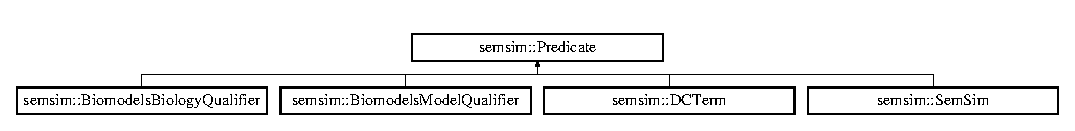
\includegraphics[height=1.308411cm]{classsemsim_1_1Predicate}
\end{center}
\end{figure}
\subsection*{Public Member Functions}
\begin{DoxyCompactItemize}
\item 
\mbox{\Hypertarget{classsemsim_1_1Predicate_a111a30f2cf259153b4f186b308b6716f}\label{classsemsim_1_1Predicate_a111a30f2cf259153b4f186b308b6716f}} 
{\bfseries Predicate} (const std\+::string \&namespace\+\_\+, std\+::string term, std\+::string prefix)
\item 
\mbox{\Hypertarget{classsemsim_1_1Predicate_a47fed0b10781d69cc6e359bcec16eb71}\label{classsemsim_1_1Predicate_a47fed0b10781d69cc6e359bcec16eb71}} 
std\+::string {\bfseries str} ()
\item 
\mbox{\Hypertarget{classsemsim_1_1Predicate_a6e4ea55d33e692cdb894940c3708cabb}\label{classsemsim_1_1Predicate_a6e4ea55d33e692cdb894940c3708cabb}} 
librdf\+\_\+node $\ast$ {\bfseries get\+Node} () const
\item 
\mbox{\Hypertarget{classsemsim_1_1Predicate_a4a1ffe837216303654416b725684b9db}\label{classsemsim_1_1Predicate_a4a1ffe837216303654416b725684b9db}} 
const std\+::vector$<$ std\+::string $>$ \& {\bfseries get\+Valid\+Terms} () const
\item 
\mbox{\Hypertarget{classsemsim_1_1Predicate_aefb90236a7934d93cce5798723f54661}\label{classsemsim_1_1Predicate_aefb90236a7934d93cce5798723f54661}} 
const std\+::string \& {\bfseries get\+Namespace} () const
\item 
\mbox{\Hypertarget{classsemsim_1_1Predicate_a1a62bbbe1ac5e3a28a15fda049d4ada4}\label{classsemsim_1_1Predicate_a1a62bbbe1ac5e3a28a15fda049d4ada4}} 
const std\+::string \& {\bfseries get\+Term} () const
\item 
\mbox{\Hypertarget{classsemsim_1_1Predicate_ad7115549cf9b25cbb665f5c2bcba67d4}\label{classsemsim_1_1Predicate_ad7115549cf9b25cbb665f5c2bcba67d4}} 
const std\+::string \& {\bfseries get\+Prefix} () const
\item 
\mbox{\Hypertarget{classsemsim_1_1Predicate_add37b6df8a8bf63600966a3ab24236d9}\label{classsemsim_1_1Predicate_add37b6df8a8bf63600966a3ab24236d9}} 
const std\+::string \& {\bfseries get\+Uri} () const
\item 
\mbox{\Hypertarget{classsemsim_1_1Predicate_aa8a95f5f9e0bffbb8d6df9c8767a6b01}\label{classsemsim_1_1Predicate_aa8a95f5f9e0bffbb8d6df9c8767a6b01}} 
void {\bfseries free\+Node} ()
\item 
\mbox{\Hypertarget{classsemsim_1_1Predicate_a56b15a4d95c7f6e4645e954e5d5d3d13}\label{classsemsim_1_1Predicate_a56b15a4d95c7f6e4645e954e5d5d3d13}} 
void {\bfseries set\+Node} (librdf\+\_\+node $\ast$node)
\end{DoxyCompactItemize}
\subsection*{Static Public Member Functions}
\begin{DoxyCompactItemize}
\item 
\mbox{\Hypertarget{classsemsim_1_1Predicate_a332f745e39155ff5884e2c98c87b548b}\label{classsemsim_1_1Predicate_a332f745e39155ff5884e2c98c87b548b}} 
static std\+::unordered\+\_\+map$<$ std\+::string, std\+::string $>$ {\bfseries namespace\+Map} ()
\item 
\mbox{\Hypertarget{classsemsim_1_1Predicate_a3e4b6a9dd8180026ef09d8234076655f}\label{classsemsim_1_1Predicate_a3e4b6a9dd8180026ef09d8234076655f}} 
static void {\bfseries verify} (std\+::vector$<$ std\+::string $>$ valid\+\_\+terms, const std\+::string \&term)
\item 
\mbox{\Hypertarget{classsemsim_1_1Predicate_a514f441587bc049f53666c55a5d645ce}\label{classsemsim_1_1Predicate_a514f441587bc049f53666c55a5d645ce}} 
static bool {\bfseries namespace\+Known} (const std\+::string \&ns)
\item 
\mbox{\Hypertarget{classsemsim_1_1Predicate_a47b3b6a018b2d1085c0feaf504e12568}\label{classsemsim_1_1Predicate_a47b3b6a018b2d1085c0feaf504e12568}} 
static void {\bfseries add\+Seen\+Namespace\+To\+Serializer} (librdf\+\_\+world $\ast$world, librdf\+\_\+serializer $\ast$serializer, librdf\+\_\+node $\ast$predicate)
\end{DoxyCompactItemize}
\subsection*{Protected Member Functions}
\begin{DoxyCompactItemize}
\item 
\mbox{\Hypertarget{classsemsim_1_1Predicate_a90af4d016315412f8fd64d9ec280b177}\label{classsemsim_1_1Predicate_a90af4d016315412f8fd64d9ec280b177}} 
{\bfseries Predicate} (librdf\+\_\+node $\ast$node)
\end{DoxyCompactItemize}
\subsection*{Protected Attributes}
\begin{DoxyCompactItemize}
\item 
\mbox{\Hypertarget{classsemsim_1_1Predicate_ad74a27f704532cdc6a80e094c2d5b3f4}\label{classsemsim_1_1Predicate_ad74a27f704532cdc6a80e094c2d5b3f4}} 
std\+::string {\bfseries namespace\+\_\+}
\item 
\mbox{\Hypertarget{classsemsim_1_1Predicate_acb9c36ea2356d2b8791a2e8ad9cf68eb}\label{classsemsim_1_1Predicate_acb9c36ea2356d2b8791a2e8ad9cf68eb}} 
std\+::string {\bfseries term\+\_\+}
\item 
\mbox{\Hypertarget{classsemsim_1_1Predicate_acb69247cf1ff304bfaec2df1755b4654}\label{classsemsim_1_1Predicate_acb69247cf1ff304bfaec2df1755b4654}} 
std\+::string {\bfseries prefix\+\_\+}
\item 
\mbox{\Hypertarget{classsemsim_1_1Predicate_a6ceaeb4b2a9a431cfdfe537be842edd2}\label{classsemsim_1_1Predicate_a6ceaeb4b2a9a431cfdfe537be842edd2}} 
std\+::string {\bfseries uri\+\_\+}
\item 
\mbox{\Hypertarget{classsemsim_1_1Predicate_a9a488e0bf03949975fa54d2de0b2fd58}\label{classsemsim_1_1Predicate_a9a488e0bf03949975fa54d2de0b2fd58}} 
librdf\+\_\+node $\ast$ {\bfseries node\+\_\+} = nullptr
\item 
\mbox{\Hypertarget{classsemsim_1_1Predicate_aaffa9838c17b7bc7c33559ef1253a594}\label{classsemsim_1_1Predicate_aaffa9838c17b7bc7c33559ef1253a594}} 
std\+::vector$<$ std\+::string $>$ \hyperlink{classsemsim_1_1Predicate_aaffa9838c17b7bc7c33559ef1253a594}{valid\+\_\+terms\+\_\+} \{\char`\"{}All\char`\"{}\}
\begin{DoxyCompactList}\small\item\em predicates can only have type uri \end{DoxyCompactList}\end{DoxyCompactItemize}


The documentation for this class was generated from the following files\+:\begin{DoxyCompactItemize}
\item 
src/semsim/Predicate.\+h\item 
src/semsim/Predicate.\+cpp\end{DoxyCompactItemize}

\hypertarget{classsemsim_1_1Query}{}\doxysection{semsim\+::Query Class Reference}
\label{classsemsim_1_1Query}\index{semsim::Query@{semsim::Query}}
\doxysubsection*{\+: variable name}
\label{_amgrp7ca1d8b10bb02d408ac42bd6ecaaf12b}%
librdf\+\_\+query\+\_\+results\+\_\+get\+\_\+binding\+\_\+value\+\_\+by\+\_\+name\+: @query\+\_\+results\+: \#librdf\+\_\+query\+\_\+results query results

Get one binding value for a given name in the current result.

Return value\+: a new \#librdf\+\_\+node binding value or N\+U\+LL on failure \begin{DoxyCompactItemize}
                                                                                  \item
                                                                                  \mbox{\Hypertarget{classsemsim_1_1Query_a25294cafa6a0df30742ba3352f736c7f}\label{classsemsim_1_1Query_a25294cafa6a0df30742ba3352f736c7f}}
                                                                                  {\bfseries Query} (Librdf\+World world, Librdf\+Model model, std\+::string query)
                                                                                  \item
                                                                                  \mbox{\Hypertarget{classsemsim_1_1Query_a3ab9edf4d5870331be842d03d6919ce0}\label{classsemsim_1_1Query_a3ab9edf4d5870331be842d03d6919ce0}}
                                                                                  {\bfseries $\sim$\+Query} ()
                                                                                  \item
                                                                                  \mbox{\Hypertarget{classsemsim_1_1Query_a83580c1b66d2d052696dd907e8594a8a}\label{classsemsim_1_1Query_a83580c1b66d2d052696dd907e8594a8a}}
                                                                                  librdf\+\_\+stream $\ast$ {\bfseries results\+As\+Lib\+Rdf\+Stream} ()
                                                                                  \item
                                                                                  \mbox{\Hypertarget{classsemsim_1_1Query_a16b43e8d44b25e0d1fba34c73c5386dc}\label{classsemsim_1_1Query_a16b43e8d44b25e0d1fba34c73c5386dc}}
                                                                                  Results\+Map {\bfseries results\+As\+Map} ()
                                                                                  \item
                                                                                  \mbox{\Hypertarget{classsemsim_1_1Query_ae44b7aff3ae00151f63cc3a355705091}\label{classsemsim_1_1Query_ae44b7aff3ae00151f63cc3a355705091}}
                                                                                  std\+::string {\bfseries results\+As\+Str} (const std\+::string \&output\+\_\+format)
\end{DoxyCompactItemize}


The documentation for this class was generated from the following files\+:\begin{DoxyCompactItemize}
                                                                              \item
                                                                              src/semsim/Query.\+h\item
                                                                              src/semsim/Query.\+cpp
\end{DoxyCompactItemize}

\hypertarget{classredland_1_1RaptorIOStream}{}\section{redland\+:\+:Raptor\+I\+O\+Stream Class Reference}
\label{classredland_1_1RaptorIOStream}\index{redland\+::\+Raptor\+I\+O\+Stream@{redland\+::\+Raptor\+I\+O\+Stream}}
\subsection*{Public Member Functions}
\begin{DoxyCompactItemize}
\item 
\mbox{\Hypertarget{classredland_1_1RaptorIOStream_a6cf2e1a9cf6c31bb37069c5b3e591509}\label{classredland_1_1RaptorIOStream_a6cf2e1a9cf6c31bb37069c5b3e591509}} 
{\bfseries Raptor\+I\+O\+Stream} (raptor\+\_\+iostream $\ast$iostream)
\item 
\mbox{\Hypertarget{classredland_1_1RaptorIOStream_adbcfcc29e030219dfd180ecb3d6c2c4b}\label{classredland_1_1RaptorIOStream_adbcfcc29e030219dfd180ecb3d6c2c4b}} 
raptor\+\_\+iostream $\ast$ {\bfseries get} () const
\end{DoxyCompactItemize}
\subsection*{Static Public Member Functions}
\begin{DoxyCompactItemize}
\item 
\mbox{\Hypertarget{classredland_1_1RaptorIOStream_ab4b78aede5b54be5a654c9b81e65452c}\label{classredland_1_1RaptorIOStream_ab4b78aede5b54be5a654c9b81e65452c}} 
static std\+::pair$<$ \hyperlink{classredland_1_1RaptorIOStream}{Raptor\+I\+O\+Stream}, void $\ast$ $>$ {\bfseries new\+I\+O\+To\+String} ()
\end{DoxyCompactItemize}


The documentation for this class was generated from the following files\+:\begin{DoxyCompactItemize}
\item 
src/redland/\+Redland\+Wrapper/src/Raptor\+I\+O\+Stream.\+h\item 
src/redland/\+Redland\+Wrapper/src/Raptor\+I\+O\+Stream.\+cpp\end{DoxyCompactItemize}

\hypertarget{classsemsim_1_1RDF}{}\section{semsim\+:\+:R\+DF Class Reference}
\label{classsemsim_1_1RDF}\index{semsim\+::\+R\+DF@{semsim\+::\+R\+DF}}
\subsection*{Public Member Functions}
\begin{DoxyCompactItemize}
\item 
\mbox{\Hypertarget{classsemsim_1_1RDF_adb3d644393c659dc3cd54b29d6bfaec0}\label{classsemsim_1_1RDF_adb3d644393c659dc3cd54b29d6bfaec0}} 
{\bfseries R\+DF} (const std\+::string \&base\+\_\+uri=\char`\"{}./Annotations.\+rdf\char`\"{}, const std\+::string \&storage\+\_\+type=\char`\"{}memory\char`\"{}, const std\+::string \&storage\+\_\+name=\char`\"{}Semsim\+Store\char`\"{}, const char $\ast$storage\+\_\+options=nullptr, const char $\ast$model\+\_\+options=nullptr)
\item 
\mbox{\Hypertarget{classsemsim_1_1RDF_aefd8c1ee16d47a49ce3e2828b7671866}\label{classsemsim_1_1RDF_aefd8c1ee16d47a49ce3e2828b7671866}} 
void {\bfseries free\+R\+DF} ()
\item 
\mbox{\Hypertarget{classsemsim_1_1RDF_a1d640ed0ead4d4699c59641a32f6a81a}\label{classsemsim_1_1RDF_a1d640ed0ead4d4699c59641a32f6a81a}} 
{\bfseries R\+DF} (const \hyperlink{classsemsim_1_1RDF}{R\+DF} \&rdf)=delete
\item 
\mbox{\Hypertarget{classsemsim_1_1RDF_ad6e8d742af0aff97c89746a8eaf50777}\label{classsemsim_1_1RDF_ad6e8d742af0aff97c89746a8eaf50777}} 
{\bfseries R\+DF} (\hyperlink{classsemsim_1_1RDF}{R\+DF} \&\&rdf) noexcept
\item 
\mbox{\Hypertarget{classsemsim_1_1RDF_a6a8c2040f0fb2be58380d09ff396f11e}\label{classsemsim_1_1RDF_a6a8c2040f0fb2be58380d09ff396f11e}} 
\hyperlink{classsemsim_1_1RDF}{R\+DF} \& {\bfseries operator=} (const \hyperlink{classsemsim_1_1RDF}{R\+DF} \&rdf)=delete
\item 
\mbox{\Hypertarget{classsemsim_1_1RDF_a0195811b138d141d7944ed475b098189}\label{classsemsim_1_1RDF_a0195811b138d141d7944ed475b098189}} 
\hyperlink{classsemsim_1_1RDF}{R\+DF} \& {\bfseries operator=} (\hyperlink{classsemsim_1_1RDF}{R\+DF} \&\&rdf) noexcept
\item 
\mbox{\Hypertarget{classsemsim_1_1RDF_aec42881cdaeeaffdc91238f03a1db2e6}\label{classsemsim_1_1RDF_aec42881cdaeeaffdc91238f03a1db2e6}} 
int {\bfseries size} () const
\item 
\mbox{\Hypertarget{classsemsim_1_1RDF_a6bbd8747ca3893339162bbb00e9f428f}\label{classsemsim_1_1RDF_a6bbd8747ca3893339162bbb00e9f428f}} 
void {\bfseries set\+Base\+Uri} (std\+::string base\+Uri)
\item 
\mbox{\Hypertarget{classsemsim_1_1RDF_ac90c8d0c73127e851825e1426ce9622e}\label{classsemsim_1_1RDF_ac90c8d0c73127e851825e1426ce9622e}} 
bool {\bfseries empty} () const
\item 
\mbox{\Hypertarget{classsemsim_1_1RDF_a3a920ea30103f06343d4714987a2b765}\label{classsemsim_1_1RDF_a3a920ea30103f06343d4714987a2b765}} 
void {\bfseries add\+From\+String} (const std\+::string \&str, const std\+::string \&format=\char`\"{}guess\char`\"{}, const std\+::string \&base\+\_\+uri=std\+::string())
\item 
\mbox{\Hypertarget{classsemsim_1_1RDF_a27497273858cca1463a612f92f332da1}\label{classsemsim_1_1RDF_a27497273858cca1463a612f92f332da1}} 
void {\bfseries add\+From\+Uri} (const std\+::string \&uri\+\_\+string, const std\+::string \&format=\char`\"{}guess\char`\"{})
\item 
\mbox{\Hypertarget{classsemsim_1_1RDF_a8cd65868da05f409c37b91acdbf33aa0}\label{classsemsim_1_1RDF_a8cd65868da05f409c37b91acdbf33aa0}} 
void {\bfseries add\+From\+File} (const std\+::string \&filename, const std\+::string \&format)
\item 
\mbox{\Hypertarget{classsemsim_1_1RDF_a493ffd6ebc12adc6c668f04f21ce2380}\label{classsemsim_1_1RDF_a493ffd6ebc12adc6c668f04f21ce2380}} 
std\+::unordered\+\_\+map$<$ std\+::string, std\+::string $>$ {\bfseries propagate\+Namespaces\+From\+Parser} (const std\+::vector$<$ std\+::string $>$ \&seen\+\_\+namespaces)
\item 
\mbox{\Hypertarget{classsemsim_1_1RDF_a762cc1d30484cd95b130526e2fab9ef3}\label{classsemsim_1_1RDF_a762cc1d30484cd95b130526e2fab9ef3}} 
std\+::string {\bfseries to\+String} (const std\+::string \&format=\char`\"{}rdfxml-\/abbrev\char`\"{}, std\+::string base\+\_\+uri=std\+::string(), const char $\ast$mime\+\_\+type=nullptr, const char $\ast$type\+\_\+uri=nullptr)
\item 
\mbox{\Hypertarget{classsemsim_1_1RDF_acf46cf3b2dbfa5828dac1e823cf972c8}\label{classsemsim_1_1RDF_acf46cf3b2dbfa5828dac1e823cf972c8}} 
\hyperlink{classsemsim_1_1Editor}{Editor} {\bfseries to\+Editor} (const std\+::string \&xml, Semsim\+Xml\+Type type)
\item 
\mbox{\Hypertarget{classsemsim_1_1RDF_a1f6a4f82d01c93be36eb5c986c1629bc}\label{classsemsim_1_1RDF_a1f6a4f82d01c93be36eb5c986c1629bc}} 
\hyperlink{classsemsim_1_1Editor}{Editor} $\ast$ {\bfseries to\+Editor\+Ptr} (const std\+::string \&xml, Semsim\+Xml\+Type type)
\item 
\mbox{\Hypertarget{classsemsim_1_1RDF_ac8286394b938d0511e7ccbf81583277c}\label{classsemsim_1_1RDF_ac8286394b938d0511e7ccbf81583277c}} 
librdf\+\_\+model $\ast$ {\bfseries get\+Model} () const
\item 
\mbox{\Hypertarget{classsemsim_1_1RDF_a92ace04b947ccd8c7c3c90a4d9d77edb}\label{classsemsim_1_1RDF_a92ace04b947ccd8c7c3c90a4d9d77edb}} 
librdf\+\_\+storage $\ast$ {\bfseries get\+Storage} () const
\end{DoxyCompactItemize}
\subsection*{Static Public Member Functions}
\begin{DoxyCompactItemize}
\item 
\mbox{\Hypertarget{classsemsim_1_1RDF_a77782a3756ed6243ee9b842c6b0f06b8}\label{classsemsim_1_1RDF_a77782a3756ed6243ee9b842c6b0f06b8}} 
static \hyperlink{classsemsim_1_1RDF}{R\+DF} {\bfseries from\+String} (const std\+::string \&str, const std\+::string \&format=\char`\"{}guess\char`\"{}, const std\+::string \&base\+\_\+uri=std\+::string())
\item 
\mbox{\Hypertarget{classsemsim_1_1RDF_a3d14028f5953a4e007cfe8f9a34b3e0d}\label{classsemsim_1_1RDF_a3d14028f5953a4e007cfe8f9a34b3e0d}} 
static \hyperlink{classsemsim_1_1RDF}{R\+DF} {\bfseries from\+Uri} (const std\+::string \&uri\+\_\+string, const std\+::string \&format=\char`\"{}guess\char`\"{})
\item 
\mbox{\Hypertarget{classsemsim_1_1RDF_ab5f969412a37a4ecad5f8485177ae561}\label{classsemsim_1_1RDF_ab5f969412a37a4ecad5f8485177ae561}} 
static \hyperlink{classsemsim_1_1RDF}{R\+DF} {\bfseries from\+File} (const std\+::string \&filename, const std\+::string \&format)
\item 
\mbox{\Hypertarget{classsemsim_1_1RDF_ab1c83f13027f0946d08dd21368706f3b}\label{classsemsim_1_1RDF_ab1c83f13027f0946d08dd21368706f3b}} 
static void {\bfseries from\+String} (\hyperlink{classsemsim_1_1RDF}{R\+DF} $\ast$rdf, const std\+::string \&str, const std\+::string \&format, const std\+::string \&base\+\_\+uri)
\end{DoxyCompactItemize}
\subsection*{Public Attributes}
\begin{DoxyCompactItemize}
\item 
\mbox{\Hypertarget{classsemsim_1_1RDF_a03a6df29bae51bba853a11d5eb433835}\label{classsemsim_1_1RDF_a03a6df29bae51bba853a11d5eb433835}} 
std\+::string {\bfseries base\+\_\+uri\+\_\+}
\item 
\mbox{\Hypertarget{classsemsim_1_1RDF_a106ee70106beb1c1304c8968470f3033}\label{classsemsim_1_1RDF_a106ee70106beb1c1304c8968470f3033}} 
Namespace\+Map {\bfseries namespaces\+\_\+}
\item 
\mbox{\Hypertarget{classsemsim_1_1RDF_af3bbb4dc4ce350bf60fc6a94bffd41b2}\label{classsemsim_1_1RDF_af3bbb4dc4ce350bf60fc6a94bffd41b2}} 
std\+::vector$<$ std\+::string $>$ {\bfseries seen\+\_\+namespaces\+\_\+}
\item 
Namespace\+Map {\bfseries default\+\_\+namespaces\+\_\+}
\end{DoxyCompactItemize}


\subsection{Member Data Documentation}
\mbox{\Hypertarget{classsemsim_1_1RDF_a9a2f19c41f10c772cb4dece71c473bd2}\label{classsemsim_1_1RDF_a9a2f19c41f10c772cb4dece71c473bd2}} 
\index{semsim\+::\+R\+DF@{semsim\+::\+R\+DF}!default\+\_\+namespaces\+\_\+@{default\+\_\+namespaces\+\_\+}}
\index{default\+\_\+namespaces\+\_\+@{default\+\_\+namespaces\+\_\+}!semsim\+::\+R\+DF@{semsim\+::\+R\+DF}}
\subsubsection{\texorpdfstring{default\+\_\+namespaces\+\_\+}{default\_namespaces\_}}
{\footnotesize\ttfamily Namespace\+Map semsim\+::\+R\+D\+F\+::default\+\_\+namespaces\+\_\+}

{\bfseries Initial value\+:}
\begin{DoxyCode}
= \{
                \{\textcolor{stringliteral}{"http://purl.org/dc/terms/"},                \textcolor{stringliteral}{"dcterms"}\},
                \{\textcolor{stringliteral}{"http://biomodels.net/biology-qualifiers/"}, \textcolor{stringliteral}{"bqbiol"}\},
                \{\textcolor{stringliteral}{"http://biomodels.net/model-qualifiers/"},   \textcolor{stringliteral}{"bqmodel"}\},
                \{\textcolor{stringliteral}{"http://www.bhi.washington.edu/semsim#"},    \textcolor{stringliteral}{"semsim"}\},
        \}
\end{DoxyCode}


The documentation for this class was generated from the following files\+:\begin{DoxyCompactItemize}
\item 
src/semsim/R\+D\+F.\+h\item 
src/semsim/R\+D\+F.\+cpp\end{DoxyCompactItemize}

\hypertarget{classRedlandLibrdfException}{}\section{Redland\+Librdf\+Exception Class Reference}
\label{classRedlandLibrdfException}\index{Redland\+Librdf\+Exception@{Redland\+Librdf\+Exception}}
Inheritance diagram for Redland\+Librdf\+Exception\+:\begin{figure}[H]
\begin{center}
\leavevmode
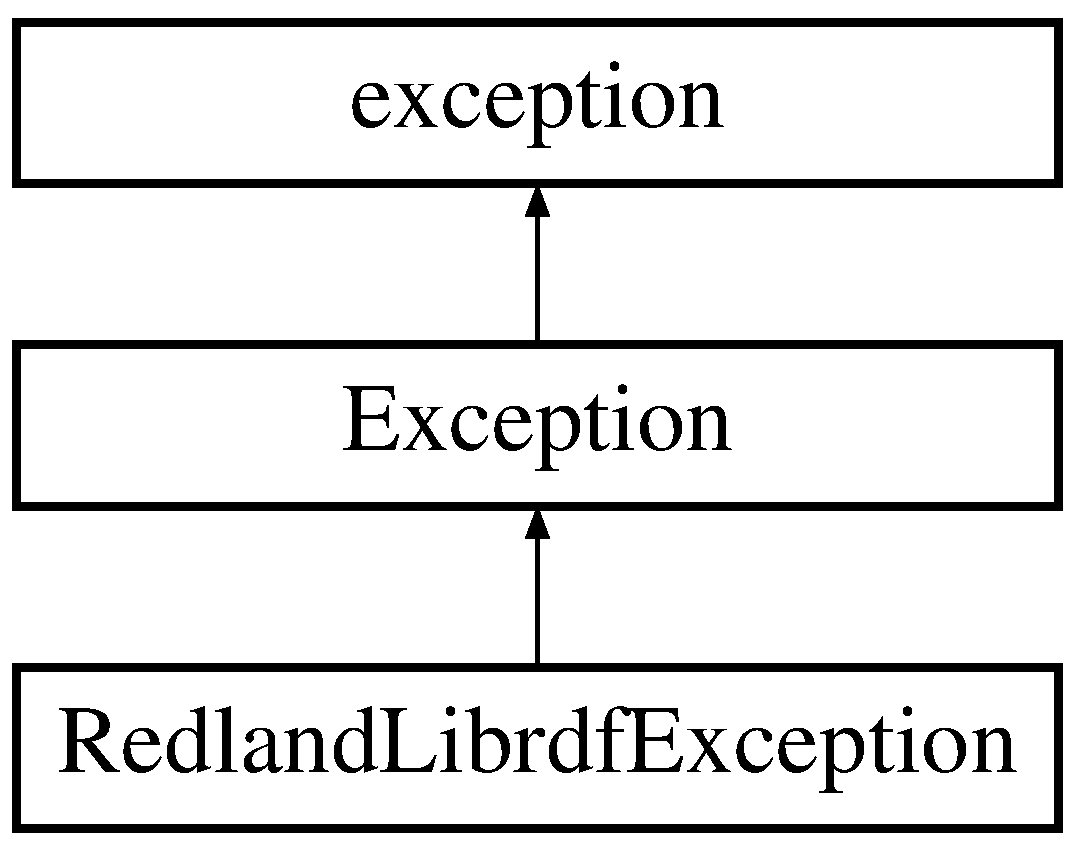
\includegraphics[height=3.000000cm]{classRedlandLibrdfException}
\end{center}
\end{figure}
\subsection*{Additional Inherited Members}


The documentation for this class was generated from the following file\+:\begin{DoxyCompactItemize}
\item 
src/redland/\+Redland\+A\+P\+I\+Wrapper/src/Librdf\+Exception.\+h\end{DoxyCompactItemize}

\hypertarget{classRedlandNullPointerException}{}\doxysection{Redland\+Null\+Pointer\+Exception Class Reference}
\label{classRedlandNullPointerException}\index{RedlandNullPointerException@{RedlandNullPointerException}}
Inheritance diagram for Redland\+Null\+Pointer\+Exception\+:\begin{figure}[H]
\begin{center}
\leavevmode
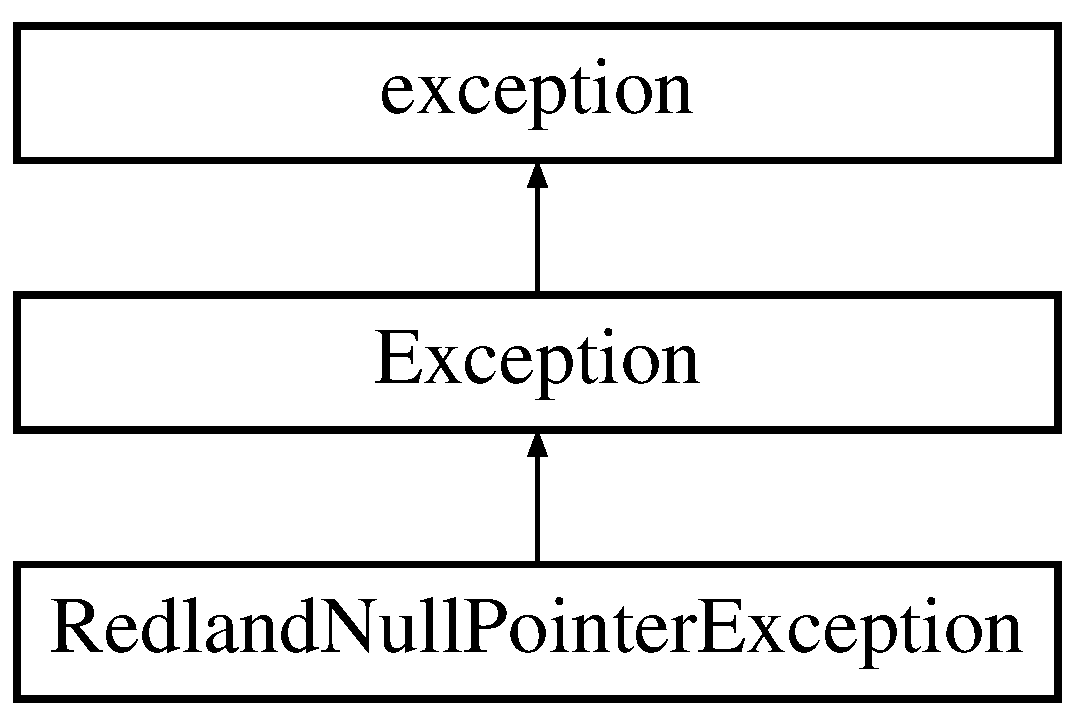
\includegraphics[height=3.000000cm]{classRedlandNullPointerException}
\end{center}
\end{figure}
\doxysubsection*{Additional Inherited Members}


The documentation for this class was generated from the following file\+:\begin{DoxyCompactItemize}
\item 
src/redland/\+Redland\+Wrapper/src/Librdf\+Exception.\+h\end{DoxyCompactItemize}

\hypertarget{classsemsim_1_1Resource}{}\doxysection{semsim\+::Resource Class Reference}
\label{classsemsim_1_1Resource}\index{semsim::Resource@{semsim::Resource}}
Inheritance diagram for semsim\+::Resource\+:\begin{figure}[H]
                                                 \begin{center}
                                                     \leavevmode
                                                     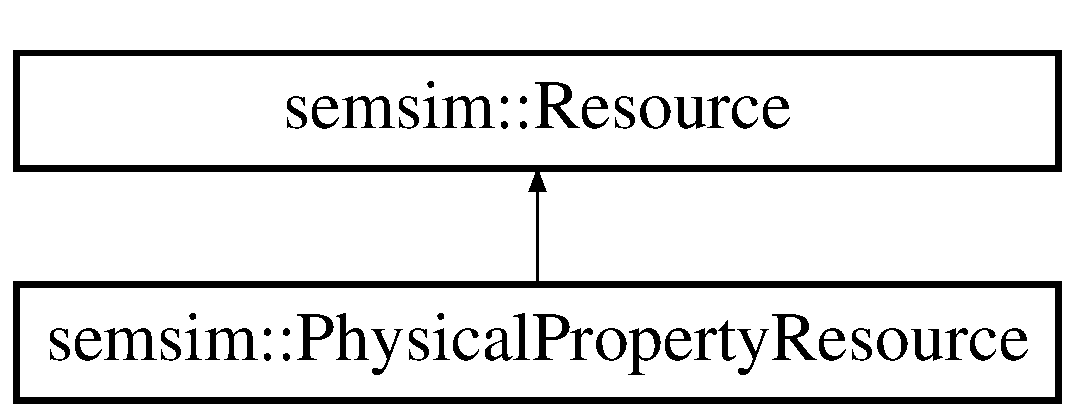
\includegraphics[height=2.000000cm]{classsemsim_1_1Resource}
                                                 \end{center}
\end{figure}
\doxysubsection*{Public Member Functions}
\begin{DoxyCompactItemize}
    \item
    \mbox{\Hypertarget{classsemsim_1_1Resource_ace808d48dfa415cef76a96049971a7d6}\label{classsemsim_1_1Resource_ace808d48dfa415cef76a96049971a7d6}}
    {\bfseries Resource} (Librdf\+World world, const \mbox{\hyperlink{classsemsim_1_1RDFLiteralNode}{R\+D\+F\+Literal\+Node}} \&node)
    \item
    \mbox{\Hypertarget{classsemsim_1_1Resource_a54c5fb0cba8d55bacfea12f16fcd9d15}\label{classsemsim_1_1Resource_a54c5fb0cba8d55bacfea12f16fcd9d15}}
    {\bfseries Resource} (Librdf\+World world, const \mbox{\hyperlink{classsemsim_1_1RDFURINode}{R\+D\+F\+U\+R\+I\+Node}} \&node)
    \item
    \mbox{\Hypertarget{classsemsim_1_1Resource_a0fafe859115b08313ff18b1eb3be521b}\label{classsemsim_1_1Resource_a0fafe859115b08313ff18b1eb3be521b}}
    {\bfseries Resource} (Librdf\+World world, const \mbox{\hyperlink{classsemsim_1_1RDFBlankNode}{R\+D\+F\+Blank\+Node}} \&node)
    \item
    \mbox{\Hypertarget{classsemsim_1_1Resource_abb0bdbdd70a34a3e8ef6ebe2b19b4ad3}\label{classsemsim_1_1Resource_abb0bdbdd70a34a3e8ef6ebe2b19b4ad3}}
    {\bfseries Resource} (Librdf\+World world, Librdf\+Node node)
    \item
    \mbox{\Hypertarget{classsemsim_1_1Resource_ab2a1eb4faf15270e7c6e6d165d751851}\label{classsemsim_1_1Resource_ab2a1eb4faf15270e7c6e6d165d751851}}
    Librdf\+Node {\bfseries get\+Node} () const
    \item
    \mbox{\Hypertarget{classsemsim_1_1Resource_ac762aa68f78bb750d71f4b109395dcfd}\label{classsemsim_1_1Resource_ac762aa68f78bb750d71f4b109395dcfd}}
    std\+::string {\bfseries str} () const
    \item
    \mbox{\Hypertarget{classsemsim_1_1Resource_a46e7e3a2b53852994f689685bb3df555}\label{classsemsim_1_1Resource_a46e7e3a2b53852994f689685bb3df555}}
    virtual bool {\bfseries is\+Set} () const
\end{DoxyCompactItemize}
\doxysubsection*{Protected Attributes}
\begin{DoxyCompactItemize}
    \item
    \mbox{\Hypertarget{classsemsim_1_1Resource_a3f51d0f7fada7133f2d4be0ec6879eff}\label{classsemsim_1_1Resource_a3f51d0f7fada7133f2d4be0ec6879eff}}
    Librdf\+World {\bfseries world\+\_\+}
    \item
    \mbox{\Hypertarget{classsemsim_1_1Resource_ac8a9754709900d4c64f79d20a38f2d1b}\label{classsemsim_1_1Resource_ac8a9754709900d4c64f79d20a38f2d1b}}
    R\+D\+F\+Node\+Ptr {\bfseries rdf\+\_\+node\+\_\+ptr\+\_\+}
\end{DoxyCompactItemize}


The documentation for this class was generated from the following files\+:\begin{DoxyCompactItemize}
                                                                              \item
                                                                              src/semsim/Resource.\+h\item
                                                                              src/semsim/Resource.\+cpp
\end{DoxyCompactItemize}

\hypertarget{classsemsim_1_1SBMLAssistant}{}\doxysection{semsim\+::S\+B\+M\+L\+Assistant Class Reference}
\label{classsemsim_1_1SBMLAssistant}\index{semsim::SBMLAssistant@{semsim::SBMLAssistant}}
Inheritance diagram for semsim\+::S\+B\+M\+L\+Assistant\+:\begin{figure}[H]
                                                              \begin{center}
                                                                  \leavevmode
                                                                  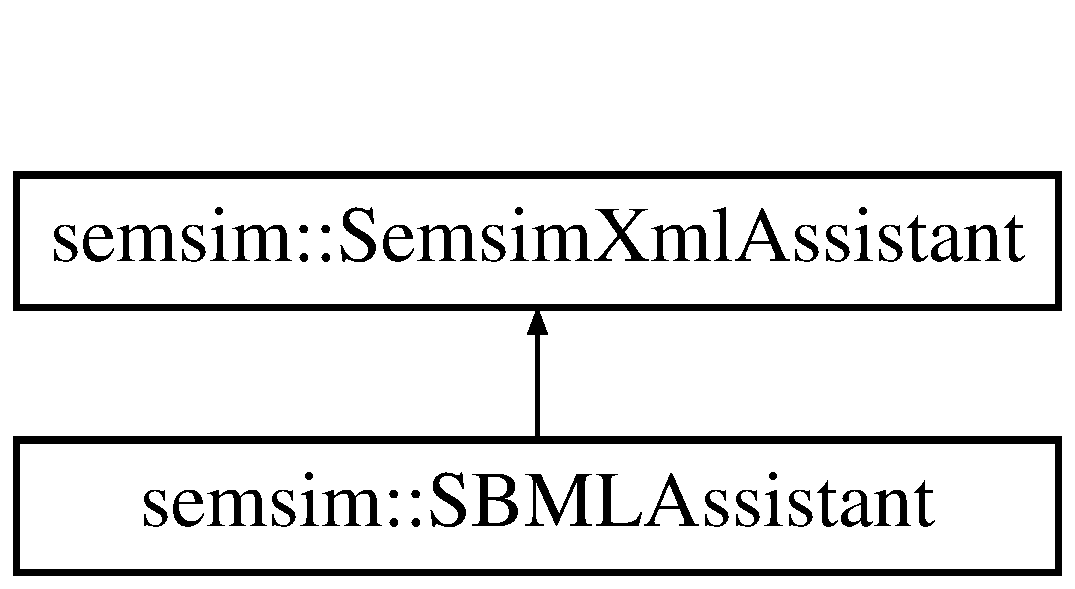
\includegraphics[height=2.000000cm]{classsemsim_1_1SBMLAssistant}
                                                              \end{center}
\end{figure}
\doxysubsection*{Public Member Functions}
\begin{DoxyCompactItemize}
    \item
    \mbox{\Hypertarget{classsemsim_1_1SBMLAssistant_a2837a0bcb04012d434795255a76beafc}\label{classsemsim_1_1SBMLAssistant_a2837a0bcb04012d434795255a76beafc}}
    const std\+::vector$<$ std\+::string $>$ \& {\bfseries get\+Valid\+Elements} () const override
    \item
    \mbox{\Hypertarget{classsemsim_1_1SBMLAssistant_a9616a091738c75e94e2ceb9f948f6b51}\label{classsemsim_1_1SBMLAssistant_a9616a091738c75e94e2ceb9f948f6b51}}
    {\bfseries Xml\+Assistant} (std\+::string xml, std\+::string base=\char`\"{}Meta\+ID\char`\"{}, int metaid\+\_\+num\+\_\+digits=4)
\end{DoxyCompactItemize}
\doxysubsection*{Protected Attributes}
\begin{DoxyCompactItemize}
    \item
    std\+::vector$<$ std\+::string $>$ {\bfseries valid\+\_\+elements\+\_\+}
\end{DoxyCompactItemize}


\doxysubsection{Member Data Documentation}
\mbox{\Hypertarget{classsemsim_1_1SBMLAssistant_a2b28803c717bcd804e9912a98caa6227}\label{classsemsim_1_1SBMLAssistant_a2b28803c717bcd804e9912a98caa6227}}
\index{semsim::SBMLAssistant@{semsim::SBMLAssistant}!valid\_elements\_@{valid\_elements\_}}
\index{valid\_elements\_@{valid\_elements\_}!semsim::SBMLAssistant@{semsim::SBMLAssistant}}
\doxysubsubsection{\texorpdfstring{valid\_elements\_}{valid\_elements\_}}
{\footnotesize\ttfamily std\+::vector$<$std\+::string$>$ semsim\+::\+S\+B\+M\+L\+Assistant\+::valid\+\_\+elements\+\_\+\hspace{0.3cm}{\ttfamily [protected]}}

{\bfseries Initial value\+:}
\begin{DoxyCode}{0}
    \DoxyCodeLine{= \{}
    \DoxyCodeLine{                \textcolor{stringliteral}{"model"},}
    \DoxyCodeLine{                \textcolor{stringliteral}{"unit"},}
    \DoxyCodeLine{                \textcolor{stringliteral}{"compartment"},}
    \DoxyCodeLine{                \textcolor{stringliteral}{"species"},}
    \DoxyCodeLine{                \textcolor{stringliteral}{"reaction"},}
    \DoxyCodeLine{                \textcolor{stringliteral}{"kineticLaw"},}
    \DoxyCodeLine{                \textcolor{stringliteral}{"localParameter"},}
    \DoxyCodeLine{        \}}

\end{DoxyCode}


The documentation for this class was generated from the following files\+:\begin{DoxyCompactItemize}
                                                                              \item
                                                                              src/semsim/Xml\+Assistant.\+h\item
                                                                              src/semsim/Xml\+Assistant.\+cpp
\end{DoxyCompactItemize}

\hypertarget{classsemsim_1_1SemSim}{}\section{semsim\+:\+:Sem\+Sim Class Reference}
\label{classsemsim_1_1SemSim}\index{semsim\+::\+Sem\+Sim@{semsim\+::\+Sem\+Sim}}
Inheritance diagram for semsim\+:\+:Sem\+Sim\+:\begin{figure}[H]
\begin{center}
\leavevmode
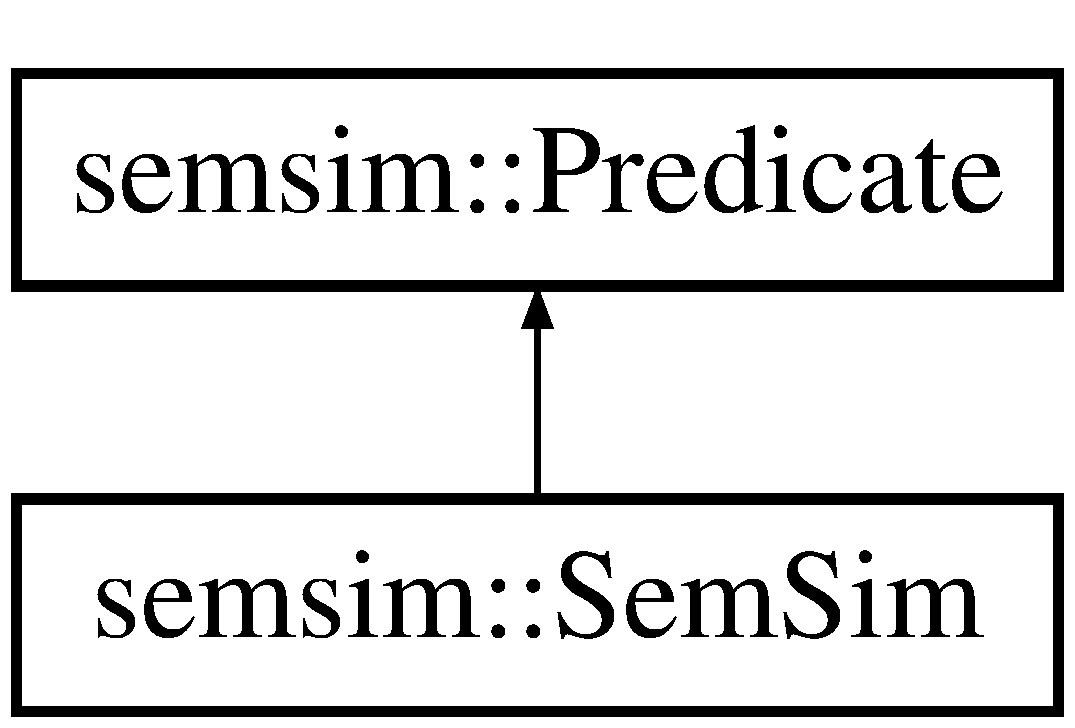
\includegraphics[height=2.000000cm]{classsemsim_1_1SemSim}
\end{center}
\end{figure}
\subsection*{Public Member Functions}
\begin{DoxyCompactItemize}
\item 
\mbox{\Hypertarget{classsemsim_1_1SemSim_ad9f48f4dde6bc27789826a29adf203ab}\label{classsemsim_1_1SemSim_ad9f48f4dde6bc27789826a29adf203ab}} 
{\bfseries Sem\+Sim} (const std\+::string \&term)
\item 
\mbox{\Hypertarget{classsemsim_1_1SemSim_a8df80cef39d98e83dab0c8c7bdae5d47}\label{classsemsim_1_1SemSim_a8df80cef39d98e83dab0c8c7bdae5d47}} 
void {\bfseries verify} ()
\end{DoxyCompactItemize}
\subsection*{Public Attributes}
\begin{DoxyCompactItemize}
\item 
std\+::vector$<$ std\+::string $>$ {\bfseries valid\+\_\+terms\+\_\+}
\end{DoxyCompactItemize}
\subsection*{Additional Inherited Members}


\subsection{Member Data Documentation}
\mbox{\Hypertarget{classsemsim_1_1SemSim_aa48e26f272827d7737f2bb9236c78102}\label{classsemsim_1_1SemSim_aa48e26f272827d7737f2bb9236c78102}} 
\index{semsim\+::\+Sem\+Sim@{semsim\+::\+Sem\+Sim}!valid\+\_\+terms\+\_\+@{valid\+\_\+terms\+\_\+}}
\index{valid\+\_\+terms\+\_\+@{valid\+\_\+terms\+\_\+}!semsim\+::\+Sem\+Sim@{semsim\+::\+Sem\+Sim}}
\subsubsection{\texorpdfstring{valid\+\_\+terms\+\_\+}{valid\_terms\_}}
{\footnotesize\ttfamily std\+::vector$<$std\+::string$>$ semsim\+::\+Sem\+Sim\+::valid\+\_\+terms\+\_\+}

{\bfseries Initial value\+:}
\begin{DoxyCode}
\{
                \textcolor{stringliteral}{"hasSourceParticipant"},
                \textcolor{stringliteral}{"hasSinkParticipant"},
                \textcolor{stringliteral}{"hasMediatorParticipant"},
                \textcolor{stringliteral}{"hasMultiplier"},
                \textcolor{stringliteral}{"hasPhysicalEntityReference"},
        \}
\end{DoxyCode}


The documentation for this class was generated from the following files\+:\begin{DoxyCompactItemize}
\item 
src/semsim/Predicate.\+h\item 
src/semsim/Predicate.\+cpp\end{DoxyCompactItemize}

\hypertarget{classsemsim_1_1SemsimUtils}{}\section{semsim\+:\+:Semsim\+Utils Class Reference}
\label{classsemsim_1_1SemsimUtils}\index{semsim\+::\+Semsim\+Utils@{semsim\+::\+Semsim\+Utils}}
\subsection*{Static Public Member Functions}
\begin{DoxyCompactItemize}
\item 
\mbox{\Hypertarget{classsemsim_1_1SemsimUtils_ac8367db330391787072c851985398805}\label{classsemsim_1_1SemsimUtils_ac8367db330391787072c851985398805}} 
static bool {\bfseries exists} (const std\+::string \&filename)
\item 
\mbox{\Hypertarget{classsemsim_1_1SemsimUtils_a1693cfd51439a6cc8c1144e82c2e83b3}\label{classsemsim_1_1SemsimUtils_a1693cfd51439a6cc8c1144e82c2e83b3}} 
static int {\bfseries remove\+File} (const std\+::string \&filename)
\item 
\mbox{\Hypertarget{classsemsim_1_1SemsimUtils_af758a31b9f4de651636587414c071059}\label{classsemsim_1_1SemsimUtils_af758a31b9f4de651636587414c071059}} 
static void {\bfseries remove\+If\+Exists} (const std\+::string \&filename)
\item 
\mbox{\Hypertarget{classsemsim_1_1SemsimUtils_a8eca0e4f3abb89c3577a8e099de8b9ba}\label{classsemsim_1_1SemsimUtils_a8eca0e4f3abb89c3577a8e099de8b9ba}} 
static void {\bfseries download} (const std\+::string \&url, std\+::string filename)
\item 
\mbox{\Hypertarget{classsemsim_1_1SemsimUtils_a07824a843bec362a8b6f7de1154068d5}\label{classsemsim_1_1SemsimUtils_a07824a843bec362a8b6f7de1154068d5}} 
static std\+::vector$<$ std\+::string $>$ {\bfseries split\+String\+By} (const std\+::string \&str, char delimiter)
\item 
\mbox{\Hypertarget{classsemsim_1_1SemsimUtils_a24671cf37888fe4b32188bd6759056d9}\label{classsemsim_1_1SemsimUtils_a24671cf37888fe4b32188bd6759056d9}} 
static std\+::string {\bfseries generate\+Unique\+Metaid} (librdf\+\_\+model $\ast$model, std\+::string metaid\+\_\+base, std\+::vector$<$ std\+::string $>$ exclusions=std\+::vector$<$ std\+::string $>$())
\item 
\mbox{\Hypertarget{classsemsim_1_1SemsimUtils_aa9435581e7fb3183edad803dbb2f5513}\label{classsemsim_1_1SemsimUtils_aa9435581e7fb3183edad803dbb2f5513}} 
static std\+::string {\bfseries add\+File\+Prefix\+To\+String} (std\+::string str)
\item 
\mbox{\Hypertarget{classsemsim_1_1SemsimUtils_a05a788ad4fb29a2f583fa1179abc15c0}\label{classsemsim_1_1SemsimUtils_a05a788ad4fb29a2f583fa1179abc15c0}} 
static std\+::string {\bfseries get\+Namespace\+From\+Uri} (const std\+::string \&uri)
\end{DoxyCompactItemize}


The documentation for this class was generated from the following files\+:\begin{DoxyCompactItemize}
\item 
src/semsim/Semsim\+Utils.\+h\item 
src/semsim/Semsim\+Utils.\+cpp\end{DoxyCompactItemize}

\hypertarget{classsemsim_1_1SemsimXmlAssistant}{}\section{semsim\+:\+:Semsim\+Xml\+Assistant Class Reference}
\label{classsemsim_1_1SemsimXmlAssistant}\index{semsim\+::\+Semsim\+Xml\+Assistant@{semsim\+::\+Semsim\+Xml\+Assistant}}
Inheritance diagram for semsim\+:\+:Semsim\+Xml\+Assistant\+:\begin{figure}[H]
\begin{center}
\leavevmode
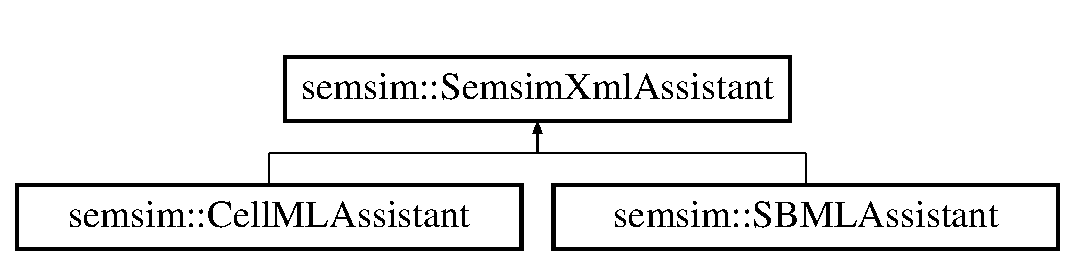
\includegraphics[height=2.000000cm]{classsemsim_1_1SemsimXmlAssistant}
\end{center}
\end{figure}
\subsection*{Public Member Functions}
\begin{DoxyCompactItemize}
\item 
\mbox{\Hypertarget{classsemsim_1_1SemsimXmlAssistant_a815b21c127616702584895612b971674}\label{classsemsim_1_1SemsimXmlAssistant_a815b21c127616702584895612b971674}} 
{\bfseries Semsim\+Xml\+Assistant} (std\+::string xml, std\+::string base=\char`\"{}Meta\+ID\char`\"{}, int metaid\+\_\+num\+\_\+digits=4)
\item 
\mbox{\Hypertarget{classsemsim_1_1SemsimXmlAssistant_a88422a4f11743c563a7ce776f4b9792a}\label{classsemsim_1_1SemsimXmlAssistant_a88422a4f11743c563a7ce776f4b9792a}} 
std\+::pair$<$ std\+::string, std\+::vector$<$ std\+::string $>$ $>$ {\bfseries add\+Meta\+Ids} ()
\item 
\mbox{\Hypertarget{classsemsim_1_1SemsimXmlAssistant_a428ad685b04bf7d4fb0beed12714c8b1}\label{classsemsim_1_1SemsimXmlAssistant_a428ad685b04bf7d4fb0beed12714c8b1}} 
virtual std\+::vector$<$ std\+::string $>$ {\bfseries get\+Valid\+Elements} () const
\end{DoxyCompactItemize}


The documentation for this class was generated from the following files\+:\begin{DoxyCompactItemize}
\item 
src/semsim/Semsim\+Xml\+Assistant.\+h\item 
src/semsim/Semsim\+Xml\+Assistant.\+cpp\end{DoxyCompactItemize}

\hypertarget{classsemsim_1_1SemsimXmlAssistantFactory}{}\section{semsim\+:\+:Semsim\+Xml\+Assistant\+Factory Class Reference}
\label{classsemsim_1_1SemsimXmlAssistantFactory}\index{semsim\+::\+Semsim\+Xml\+Assistant\+Factory@{semsim\+::\+Semsim\+Xml\+Assistant\+Factory}}
\subsection*{Static Public Member Functions}
\begin{DoxyCompactItemize}
\item 
\mbox{\Hypertarget{classsemsim_1_1SemsimXmlAssistantFactory_af24bed5c527a0a05d0fe579f1faa6dfd}\label{classsemsim_1_1SemsimXmlAssistantFactory_af24bed5c527a0a05d0fe579f1faa6dfd}} 
static Xml\+Assistant\+Ptr {\bfseries generate} (const std\+::string \&xml, Semsim\+Xml\+Type type)
\end{DoxyCompactItemize}


The documentation for this class was generated from the following files\+:\begin{DoxyCompactItemize}
\item 
src/semsim/Semsim\+Xml\+Assistant.\+h\item 
src/semsim/Semsim\+Xml\+Assistant.\+cpp\end{DoxyCompactItemize}

\hypertarget{classsemsim_1_1SinkParticipant}{}\section{semsim\+:\+:Sink\+Participant Class Reference}
\label{classsemsim_1_1SinkParticipant}\index{semsim\+::\+Sink\+Participant@{semsim\+::\+Sink\+Participant}}
Inheritance diagram for semsim\+:\+:Sink\+Participant\+:\begin{figure}[H]
\begin{center}
\leavevmode
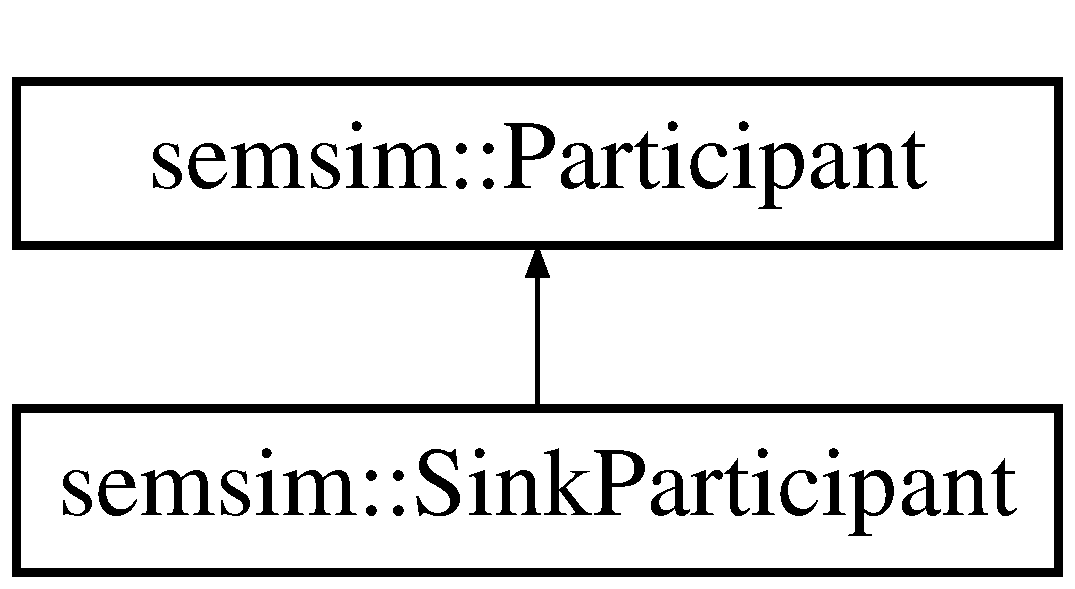
\includegraphics[height=2.000000cm]{classsemsim_1_1SinkParticipant}
\end{center}
\end{figure}
\subsection*{Public Member Functions}
\begin{DoxyCompactItemize}
\item 
\mbox{\Hypertarget{classsemsim_1_1SinkParticipant_adf61163edf45c215ad1f252d3dbf7490}\label{classsemsim_1_1SinkParticipant_adf61163edf45c215ad1f252d3dbf7490}} 
{\bfseries Sink\+Participant} (librdf\+\_\+model $\ast$model, std\+::string subject, double multiplier, std\+::string physical\+Entity\+Reference)
\end{DoxyCompactItemize}


The documentation for this class was generated from the following files\+:\begin{DoxyCompactItemize}
\item 
src/semsim/Participant.\+h\item 
src/semsim/Participant.\+cpp\end{DoxyCompactItemize}

\hypertarget{classsemsim_1_1SourceParticipant}{}\section{semsim\+:\+:Source\+Participant Class Reference}
\label{classsemsim_1_1SourceParticipant}\index{semsim\+::\+Source\+Participant@{semsim\+::\+Source\+Participant}}
Inheritance diagram for semsim\+:\+:Source\+Participant\+:\begin{figure}[H]
\begin{center}
\leavevmode
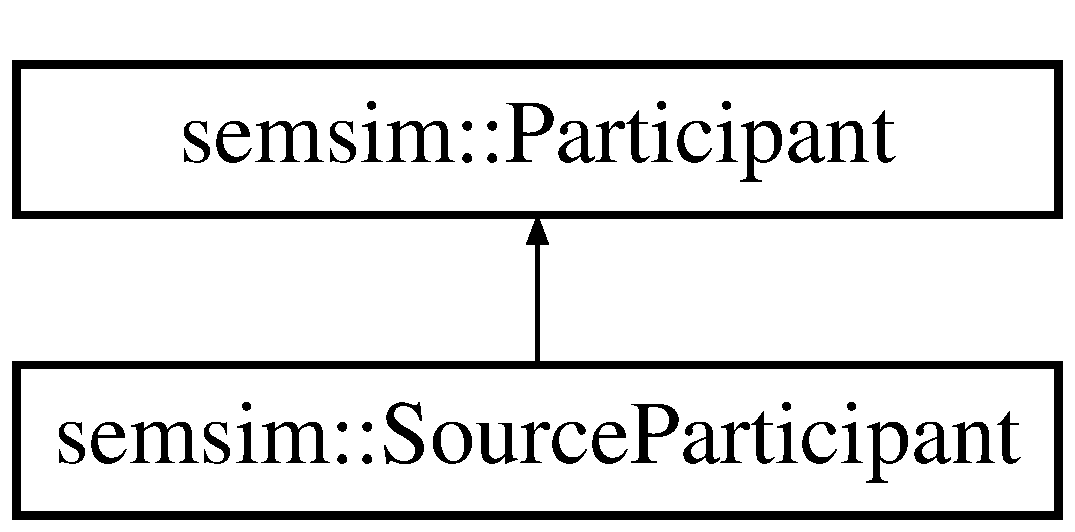
\includegraphics[height=2.000000cm]{classsemsim_1_1SourceParticipant}
\end{center}
\end{figure}
\subsection*{Public Member Functions}
\begin{DoxyCompactItemize}
\item 
\mbox{\Hypertarget{classsemsim_1_1SourceParticipant_a7e942f26b1bf916f0441d353f80833a1}\label{classsemsim_1_1SourceParticipant_a7e942f26b1bf916f0441d353f80833a1}} 
{\bfseries Source\+Participant} (librdf\+\_\+model $\ast$model, std\+::string subject, double multiplier, std\+::string physical\+Entity\+Reference)
\end{DoxyCompactItemize}


The documentation for this class was generated from the following files\+:\begin{DoxyCompactItemize}
\item 
src/semsim/Participant.\+h\item 
src/semsim/Participant.\+cpp\end{DoxyCompactItemize}

\hypertarget{classsemsim_1_1Subject}{}\doxysection{semsim\+::Subject Class Reference}
\label{classsemsim_1_1Subject}\index{semsim::Subject@{semsim::Subject}}
\doxysubsection*{Public Member Functions}
\begin{DoxyCompactItemize}
    \item
    \mbox{\Hypertarget{classsemsim_1_1Subject_aacdb633d3dedfafe4dfdfeb5f3dd0274}\label{classsemsim_1_1Subject_aacdb633d3dedfafe4dfdfeb5f3dd0274}}
    {\bfseries Subject} (Librdf\+World world, const \mbox{\hyperlink{classsemsim_1_1RDFBlankNode}{R\+D\+F\+Blank\+Node}} \&node)
    \item
    \mbox{\Hypertarget{classsemsim_1_1Subject_ad845337adfa0dd31c0877419c56e59ae}\label{classsemsim_1_1Subject_ad845337adfa0dd31c0877419c56e59ae}}
    {\bfseries Subject} (Librdf\+World world, const \mbox{\hyperlink{classsemsim_1_1RDFURINode}{R\+D\+F\+U\+R\+I\+Node}} \&node)
    \item
    \mbox{\Hypertarget{classsemsim_1_1Subject_a8c78cd99c5a15b9ccb2d6d88fe7f6795}\label{classsemsim_1_1Subject_a8c78cd99c5a15b9ccb2d6d88fe7f6795}}
    {\bfseries Subject} (const \mbox{\hyperlink{classsemsim_1_1RDFNode}{R\+D\+F\+Node}} \&node)
    \item
    \mbox{\Hypertarget{classsemsim_1_1Subject_aeb6a8e09e0056852e1fc0c5b13404ab4}\label{classsemsim_1_1Subject_aeb6a8e09e0056852e1fc0c5b13404ab4}}
    Librdf\+Node {\bfseries get\+Node} () const
    \item
    \mbox{\Hypertarget{classsemsim_1_1Subject_a4244a40a89fb9a3dd6ffff35cd95f7ca}\label{classsemsim_1_1Subject_a4244a40a89fb9a3dd6ffff35cd95f7ca}}
    std\+::string {\bfseries str} () const
    \item
    \mbox{\Hypertarget{classsemsim_1_1Subject_aecfc41aed32eb5a2a5c5eadc814192d2}\label{classsemsim_1_1Subject_aecfc41aed32eb5a2a5c5eadc814192d2}}
    bool {\bfseries is\+Set} () const
\end{DoxyCompactItemize}
\doxysubsection*{Static Public Member Functions}
\begin{DoxyCompactItemize}
    \item
    \mbox{\Hypertarget{classsemsim_1_1Subject_adfc6b48f5596aa5b706cdf35a2e98251}\label{classsemsim_1_1Subject_adfc6b48f5596aa5b706cdf35a2e98251}}
    static \mbox{\hyperlink{classsemsim_1_1Subject}{Subject}} {\bfseries from\+Uri} (Librdf\+World world, const std\+::string \&uri)
    \item
    \mbox{\Hypertarget{classsemsim_1_1Subject_ae99f64489a5b5ea33de244a43203bdce}\label{classsemsim_1_1Subject_ae99f64489a5b5ea33de244a43203bdce}}
    static \mbox{\hyperlink{classsemsim_1_1Subject}{Subject}} {\bfseries from\+Blank} (Librdf\+World world, const std\+::string \&blank)
\end{DoxyCompactItemize}


The documentation for this class was generated from the following files\+:\begin{DoxyCompactItemize}
                                                                              \item
                                                                              src/semsim/Subject.\+h\item
                                                                              src/semsim/Subject.\+cpp
\end{DoxyCompactItemize}

\hypertarget{classsemsim_1_1Triple}{}\doxysection{semsim\+::Triple Class Reference}
\label{classsemsim_1_1Triple}\index{semsim::Triple@{semsim::Triple}}
\doxysubsection*{Public Member Functions}
\begin{DoxyCompactItemize}
    \item
    \mbox{\Hypertarget{classsemsim_1_1Triple_a7bb8058c12d060f472064ca759c64a18}\label{classsemsim_1_1Triple_a7bb8058c12d060f472064ca759c64a18}}
    {\bfseries Triple} (Librdf\+World world)
    \item
    \mbox{\Hypertarget{classsemsim_1_1Triple_ad9425f62a08193a002987df799fe900f}\label{classsemsim_1_1Triple_ad9425f62a08193a002987df799fe900f}}
    {\bfseries Triple} (Librdf\+World world, \mbox{\hyperlink{classsemsim_1_1Subject}{Subject}} subject, Predicate\+Ptr predicate\+\_\+ptr, \mbox{\hyperlink{classsemsim_1_1Resource}{Resource}} resource)
    \item
    \mbox{\Hypertarget{classsemsim_1_1Triple_ac43f5c20b96fa58bffc623d5564f1b20}\label{classsemsim_1_1Triple_ac43f5c20b96fa58bffc623d5564f1b20}}
    void {\bfseries set\+Subject} (const \mbox{\hyperlink{classsemsim_1_1Subject}{Subject}} \&subject)
    \item
    \mbox{\Hypertarget{classsemsim_1_1Triple_a012df707ae8deb825c99fec968008e98}\label{classsemsim_1_1Triple_a012df707ae8deb825c99fec968008e98}}
    void {\bfseries set\+Predicate\+Ptr} (const Predicate\+Ptr \&predicate\+Ptr)
    \item
    \mbox{\Hypertarget{classsemsim_1_1Triple_a8bf5c327d3a50a57496d34e9f89357a6}\label{classsemsim_1_1Triple_a8bf5c327d3a50a57496d34e9f89357a6}}
    void {\bfseries set\+Resource} (const \mbox{\hyperlink{classsemsim_1_1Resource}{Resource}} \&resource)
    \item
    \mbox{\Hypertarget{classsemsim_1_1Triple_ac37873eb3de4284c2320c6f171af2923}\label{classsemsim_1_1Triple_ac37873eb3de4284c2320c6f171af2923}}
    {\bfseries Triple} (Librdf\+World world, \mbox{\hyperlink{classsemsim_1_1Subject}{Subject}} subject, const \mbox{\hyperlink{classsemsim_1_1Predicate}{Predicate}} \&predicate, \mbox{\hyperlink{classsemsim_1_1Resource}{Resource}} resource)
    \item
    \mbox{\Hypertarget{classsemsim_1_1Triple_a491648181ba7849276e41cff17df914d}\label{classsemsim_1_1Triple_a491648181ba7849276e41cff17df914d}}
    \mbox{\hyperlink{classsemsim_1_1Subject}{Subject}} {\bfseries get\+Subject} () const
    \item
    \mbox{\Hypertarget{classsemsim_1_1Triple_a807e29d9a3e772c371eb8fae5160a5eb}\label{classsemsim_1_1Triple_a807e29d9a3e772c371eb8fae5160a5eb}}
    Predicate\+Ptr {\bfseries get\+Predicate\+Ptr} () const
    \item
    \mbox{\Hypertarget{classsemsim_1_1Triple_ab67b033916f5590528aa30a853b44083}\label{classsemsim_1_1Triple_ab67b033916f5590528aa30a853b44083}}
    \mbox{\hyperlink{classsemsim_1_1Resource}{Resource}} {\bfseries get\+Resource} () const
    \item
    \mbox{\Hypertarget{classsemsim_1_1Triple_af6ab8db4c8e40709def27458a25b7b16}\label{classsemsim_1_1Triple_af6ab8db4c8e40709def27458a25b7b16}}
    Librdf\+Statement {\bfseries to\+Statement} ()
    \item
    \mbox{\Hypertarget{classsemsim_1_1Triple_a5eb4b44cc9941223ea5c2887282512ba}\label{classsemsim_1_1Triple_a5eb4b44cc9941223ea5c2887282512ba}}
    std\+::string {\bfseries str} (std\+::string format=\char`\"{}rdfxml-\/abbrev\char`\"{}, std\+::string base=\char`\"{}file\+://./annotations.\+rdf\char`\"{})
    \item
    \mbox{\Hypertarget{classsemsim_1_1Triple_ad2b2ab0b15a970f5dc95a25e1ec61f1f}\label{classsemsim_1_1Triple_ad2b2ab0b15a970f5dc95a25e1ec61f1f}}
    \mbox{\hyperlink{classsemsim_1_1Triple}{Triple}} \& {\bfseries set\+About} (const std\+::string \&about)
    \item
    \mbox{\Hypertarget{classsemsim_1_1Triple_af39ecc1713db90ccfbad436eb52fe900}\label{classsemsim_1_1Triple_af39ecc1713db90ccfbad436eb52fe900}}
    \mbox{\hyperlink{classsemsim_1_1Triple}{Triple}} \& {\bfseries set\+Predicate} (const std\+::string \&namespace\+\_\+, const std\+::string \&term)
    \item
    \mbox{\Hypertarget{classsemsim_1_1Triple_a73909af1fa338a2888f935835aa805f7}\label{classsemsim_1_1Triple_a73909af1fa338a2888f935835aa805f7}}
    \mbox{\hyperlink{classsemsim_1_1Triple}{Triple}} \& {\bfseries set\+Predicate\+New} (const std\+::string \&namespace\+\_\+, const std\+::string \&term, const std\+::string \&prefix)
    \item
    \mbox{\Hypertarget{classsemsim_1_1Triple_ad85dc3e3538da54fb96387a3135b8f78}\label{classsemsim_1_1Triple_ad85dc3e3538da54fb96387a3135b8f78}}
    \mbox{\hyperlink{classsemsim_1_1Triple}{Triple}} \& {\bfseries set\+Resource\+Literal} (const std\+::string \&literal)
    \item
    \mbox{\Hypertarget{classsemsim_1_1Triple_a09a6b7c88633a87f489a8f125897935a}\label{classsemsim_1_1Triple_a09a6b7c88633a87f489a8f125897935a}}
    \mbox{\hyperlink{classsemsim_1_1Triple}{Triple}} \& {\bfseries set\+Resource\+Uri} (const std\+::string \&identifiers\+\_\+uri)
    \item
    \mbox{\Hypertarget{classsemsim_1_1Triple_a5f62f4d7c1dc8877fa7861d0b399c696}\label{classsemsim_1_1Triple_a5f62f4d7c1dc8877fa7861d0b399c696}}
    \mbox{\hyperlink{classsemsim_1_1Triple}{Triple}} \& {\bfseries set\+Resource\+Blank} (const std\+::string \&blank\+\_\+id)
    \item
    \mbox{\Hypertarget{classsemsim_1_1Triple_a972f806fbf6e71f60f6b6b7ba433c79c}\label{classsemsim_1_1Triple_a972f806fbf6e71f60f6b6b7ba433c79c}}
    std\+::string {\bfseries get\+About} () const
\end{DoxyCompactItemize}
\doxysubsection*{Static Public Member Functions}
\begin{DoxyCompactItemize}
    \item
    \mbox{\Hypertarget{classsemsim_1_1Triple_abecbc59be28dca3e501ce8ed112e6198}\label{classsemsim_1_1Triple_abecbc59be28dca3e501ce8ed112e6198}}
    static \mbox{\hyperlink{classsemsim_1_1Triple}{Triple}} {\bfseries from\+Statement} (Librdf\+World world, Librdf\+Statement statement)
\end{DoxyCompactItemize}
\doxysubsection*{Protected Attributes}
\begin{DoxyCompactItemize}
    \item
    \mbox{\Hypertarget{classsemsim_1_1Triple_a27380e3a61d2bc63411ae40b9afec276}\label{classsemsim_1_1Triple_a27380e3a61d2bc63411ae40b9afec276}}
    Librdf\+World {\bfseries world\+\_\+} \{\}
    \item
    \mbox{\Hypertarget{classsemsim_1_1Triple_a071c53ad2a1b32d696cba777216ac6d8}\label{classsemsim_1_1Triple_a071c53ad2a1b32d696cba777216ac6d8}}
    \mbox{\hyperlink{classsemsim_1_1Subject}{Subject}} {\bfseries subject\+\_\+}
    \item
    \mbox{\Hypertarget{classsemsim_1_1Triple_a51da40a3bc7b14f59d970272cec4d541}\label{classsemsim_1_1Triple_a51da40a3bc7b14f59d970272cec4d541}}
    Predicate\+Ptr {\bfseries predicate\+\_\+ptr\+\_\+}
    \item
    \mbox{\Hypertarget{classsemsim_1_1Triple_ac33b956ea00a7330aaf46f4af9743de7}\label{classsemsim_1_1Triple_ac33b956ea00a7330aaf46f4af9743de7}}
    \mbox{\hyperlink{classsemsim_1_1Resource}{Resource}} {\bfseries resource\+\_\+}
\end{DoxyCompactItemize}


The documentation for this class was generated from the following files\+:\begin{DoxyCompactItemize}
                                                                              \item
                                                                              src/semsim/Triple.\+h\item
                                                                              src/semsim/Triple.\+cpp
\end{DoxyCompactItemize}

\hypertarget{classsemsim_1_1Triples}{}\section{semsim\+:\+:Triples Class Reference}
\label{classsemsim_1_1Triples}\index{semsim\+::\+Triples@{semsim\+::\+Triples}}
\subsection*{Public Member Functions}
\begin{DoxyCompactItemize}
\item 
\mbox{\Hypertarget{classsemsim_1_1Triples_a620eba7d105212f69f762e9614c82928}\label{classsemsim_1_1Triples_a620eba7d105212f69f762e9614c82928}} 
{\bfseries Triples} (\hyperlink{classsemsim_1_1Triple}{Triple} triple)
\item 
\mbox{\Hypertarget{classsemsim_1_1Triples_a09d81ba233bf8a3ca5a9ede2df74c825}\label{classsemsim_1_1Triples_a09d81ba233bf8a3ca5a9ede2df74c825}} 
{\bfseries Triples} (std\+::vector$<$ \hyperlink{classsemsim_1_1Triple}{Triple} $>$ triples)
\item 
\mbox{\Hypertarget{classsemsim_1_1Triples_a6a93d787c250b81592bb9b5fa30fdec2}\label{classsemsim_1_1Triples_a6a93d787c250b81592bb9b5fa30fdec2}} 
void {\bfseries push\+\_\+back} (\hyperlink{classsemsim_1_1Triple}{Triple} triple)
\item 
\mbox{\Hypertarget{classsemsim_1_1Triples_a2387f43385258c96bd68ca38d1a53c94}\label{classsemsim_1_1Triples_a2387f43385258c96bd68ca38d1a53c94}} 
void {\bfseries emplace\+\_\+back} (\hyperlink{classsemsim_1_1Subject}{Subject} subject, const Predicate\+Ptr \&predicate\+Ptr, const \hyperlink{classsemsim_1_1Resource}{Resource} \&resource)
\item 
\mbox{\Hypertarget{classsemsim_1_1Triples_a69c8a69a0dcffc60e510b731a0ffec69}\label{classsemsim_1_1Triples_a69c8a69a0dcffc60e510b731a0ffec69}} 
void {\bfseries emplace\+\_\+back} (\hyperlink{classsemsim_1_1Subject}{Subject} subject, const \hyperlink{classsemsim_1_1Predicate}{Predicate} \&predicate, const \hyperlink{classsemsim_1_1Resource}{Resource} \&resource)
\item 
\mbox{\Hypertarget{classsemsim_1_1Triples_a139321c0554ce0cf98d2fccc82599653}\label{classsemsim_1_1Triples_a139321c0554ce0cf98d2fccc82599653}} 
void {\bfseries emplace\+\_\+back} (\hyperlink{classsemsim_1_1Subject}{Subject} subject, \hyperlink{classsemsim_1_1BiomodelsBiologyQualifier}{Biomodels\+Biology\+Qualifier} predicate, const \hyperlink{classsemsim_1_1Resource}{Resource} \&resource)
\item 
\mbox{\Hypertarget{classsemsim_1_1Triples_a7a7839f22cac425a78e6b4c95fa7d423}\label{classsemsim_1_1Triples_a7a7839f22cac425a78e6b4c95fa7d423}} 
void {\bfseries emplace\+\_\+back} (\hyperlink{classsemsim_1_1Subject}{Subject} subject, \hyperlink{classsemsim_1_1BiomodelsModelQualifier}{Biomodels\+Model\+Qualifier} predicate, const \hyperlink{classsemsim_1_1Resource}{Resource} \&resource)
\item 
\mbox{\Hypertarget{classsemsim_1_1Triples_a83049cf0e93d420a318bd041ec5410fb}\label{classsemsim_1_1Triples_a83049cf0e93d420a318bd041ec5410fb}} 
void {\bfseries emplace\+\_\+back} (\hyperlink{classsemsim_1_1Subject}{Subject} subject, \hyperlink{classsemsim_1_1DCTerm}{D\+C\+Term} predicate, const \hyperlink{classsemsim_1_1Resource}{Resource} \&resource)
\item 
\mbox{\Hypertarget{classsemsim_1_1Triples_aceaa9df401907b19d286ae8be29a4ed1}\label{classsemsim_1_1Triples_aceaa9df401907b19d286ae8be29a4ed1}} 
void {\bfseries emplace\+\_\+back} (\hyperlink{classsemsim_1_1Subject}{Subject} subject, \hyperlink{classsemsim_1_1SemSim}{Sem\+Sim} predicate, const \hyperlink{classsemsim_1_1Resource}{Resource} \&resource)
\item 
\mbox{\Hypertarget{classsemsim_1_1Triples_a0cdb24ded3d2c8bcec95a41cfd8f14ec}\label{classsemsim_1_1Triples_a0cdb24ded3d2c8bcec95a41cfd8f14ec}} 
void {\bfseries emplace\+\_\+back} (librdf\+\_\+node $\ast$subject, librdf\+\_\+node $\ast$predicate, librdf\+\_\+node $\ast$resource)
\item 
\mbox{\Hypertarget{classsemsim_1_1Triples_a95177537847688d33f83302a65767982}\label{classsemsim_1_1Triples_a95177537847688d33f83302a65767982}} 
std\+::vector$<$ std\+::string $>$ {\bfseries get\+Subjects\+Str} ()
\item 
\mbox{\Hypertarget{classsemsim_1_1Triples_aa51480fb718cd5b47a2c96fc99a10c2c}\label{classsemsim_1_1Triples_aa51480fb718cd5b47a2c96fc99a10c2c}} 
std\+::vector$<$ std\+::string $>$ {\bfseries get\+Predicates} ()
\item 
\mbox{\Hypertarget{classsemsim_1_1Triples_ae4e47c0881214aec04987fada026f9ae}\label{classsemsim_1_1Triples_ae4e47c0881214aec04987fada026f9ae}} 
std\+::vector$<$ std\+::string $>$ {\bfseries get\+Resources} ()
\item 
\mbox{\Hypertarget{classsemsim_1_1Triples_a9787be0290ba6519cc4f71b28ce280f6}\label{classsemsim_1_1Triples_a9787be0290ba6519cc4f71b28ce280f6}} 
int {\bfseries size} ()
\item 
\mbox{\Hypertarget{classsemsim_1_1Triples_a7c107f7dd600189cff1b0abf6bdd5e72}\label{classsemsim_1_1Triples_a7c107f7dd600189cff1b0abf6bdd5e72}} 
Shared\+Triple\+Vector\+::iterator {\bfseries begin} ()
\item 
\mbox{\Hypertarget{classsemsim_1_1Triples_a9551a7d3ecc878b6ff87ddd2c52d6481}\label{classsemsim_1_1Triples_a9551a7d3ecc878b6ff87ddd2c52d6481}} 
Shared\+Triple\+Vector\+::iterator {\bfseries end} ()
\item 
\mbox{\Hypertarget{classsemsim_1_1Triples_a3fce442d97360b0c6ccb55fdf11f0bf2}\label{classsemsim_1_1Triples_a3fce442d97360b0c6ccb55fdf11f0bf2}} 
std\+::string {\bfseries str} (const std\+::string \&format=\char`\"{}rdfxml-\/abbrev\char`\"{}, std\+::string base=\char`\"{}file\+://./annotations.\+rdf\char`\"{})
\item 
\mbox{\Hypertarget{classsemsim_1_1Triples_afb9f000468cbe6c68f6c5706f0b2c781}\label{classsemsim_1_1Triples_afb9f000468cbe6c68f6c5706f0b2c781}} 
void {\bfseries push\+\_\+back} (const std\+::shared\+\_\+ptr$<$ \hyperlink{classsemsim_1_1Triple}{Triple} $>$ \&triple)
\end{DoxyCompactItemize}


The documentation for this class was generated from the following files\+:\begin{DoxyCompactItemize}
\item 
src/semsim/Triples.\+h\item 
src/semsim/Triples.\+cpp\end{DoxyCompactItemize}

\hypertarget{classsemsim_1_1ValueException}{}\section{semsim\+:\+:Value\+Exception Class Reference}
\label{classsemsim_1_1ValueException}\index{semsim\+::\+Value\+Exception@{semsim\+::\+Value\+Exception}}
Inheritance diagram for semsim\+:\+:Value\+Exception\+:\begin{figure}[H]
\begin{center}
\leavevmode
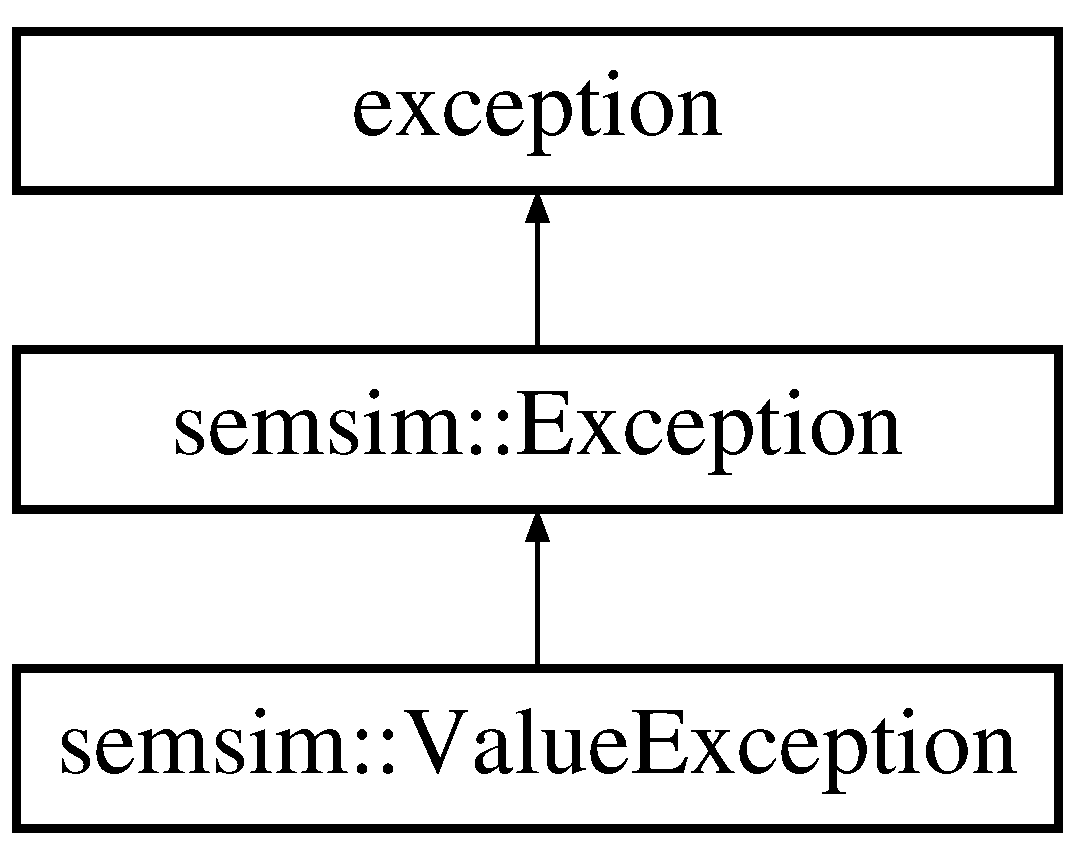
\includegraphics[height=3.000000cm]{classsemsim_1_1ValueException}
\end{center}
\end{figure}
\subsection*{Additional Inherited Members}


The documentation for this class was generated from the following file\+:\begin{DoxyCompactItemize}
\item 
src/semsim/Error.\+h\end{DoxyCompactItemize}

\hypertarget{classredland_1_1World}{}\section{redland\+:\+:World Class Reference}
\label{classredland_1_1World}\index{redland\+::\+World@{redland\+::\+World}}
\subsection*{Static Public Member Functions}
\begin{DoxyCompactItemize}
\item 
\mbox{\Hypertarget{classredland_1_1World_ad7618363c9b7da4c87367707c1a159d7}\label{classredland_1_1World_ad7618363c9b7da4c87367707c1a159d7}} 
static librdf\+\_\+world $\ast$ {\bfseries get\+World} ()
\item 
\mbox{\Hypertarget{classredland_1_1World_aac0ce4018279ced7b38a36d74bb10cec}\label{classredland_1_1World_aac0ce4018279ced7b38a36d74bb10cec}} 
static raptor\+\_\+world $\ast$ {\bfseries get\+Raptor} ()
\item 
\mbox{\Hypertarget{classredland_1_1World_ade64918f10ee6ee0f5b8a0cb2e01666b}\label{classredland_1_1World_ade64918f10ee6ee0f5b8a0cb2e01666b}} 
static void {\bfseries free} (librdf\+\_\+world $\ast$world)
\end{DoxyCompactItemize}


The documentation for this class was generated from the following files\+:\begin{DoxyCompactItemize}
\item 
src/redland/\+Redland\+A\+P\+I\+Wrapper/src/World.\+h\item 
src/redland/\+Redland\+A\+P\+I\+Wrapper/src/World.\+cpp\end{DoxyCompactItemize}

%--- End generated contents ---

% Index
\backmatter
\newpage
\phantomsection
\clearemptydoublepage
\addcontentsline{toc}{chapter}{Index}
\printindex

\end{document}
